\chapter{Implementation and discussion} \label{chap: Result}

In this chapter, the use cases for implementation are explained 
in chapter \ref{chap: Usecase} and the results of the performance 
tests based on assumptions 
and the BMW use cases to verify the feasibility of the methods presented 
in chapter \ref{chap: Meth} will be discussed. The tests will be divided into 
two parts: local \gls{mas} (section \ref{chap: Result-Internal}) and 
global \gls{dt} (section \ref{chap: Result-External}), as previously mentioned in 
chapter \ref{chap: Meth}. Both of them are tested under a 5G Network in the lab.

\section{Use case Wittenstein and BMW}\label{chap: Usecase}
To get to the point quickly, some prior knowledge will be provided. 

This work is under the ongoing flagship project KI.FABRIK, aims to 
find solutions to enable direct physical interactions between humans and 
machines. The current status of the studies is mainly based on two use 
cases: Wittenstein and BMW use case. 

The Wittenstein gearbox assembly use case mainly involves the cooperation of different 
robots, including a mobile picking robot that collects assembly parts from 
the supermarket cell with a shop list and then puts them into a standard box (KLT). 
After that, the picking robot will move the standard box to the assembly line for 
the assembly task. The assembly tasks are divided into different subtasks for 
multiple assembly robots. After finishing each subtask, the picking robot 
will come again and move the semi-finished product to the next assembly station. 
In case of emergency, teleoperations will be performed to fix the 
errors. 

Similarly, the BMW use case also includes assembly tasks, but for the cockpit 
pre-assembly. Instead of assembling gearbox parts, a more delicate wiring task 
is performed. The production consists of four parts: the pre-assembly of the cover, 
the quality assurance with agent 
assistance and \gls{dt} as a checksum, the fitting of the cover to the cockpit, and 
finally, the quality inspection. All these tasks involve the coworking of 
multiple assembly robots and the assistance of teleoperations. Additionally, 
smart logistics are responsible for delivering parts to 
specific assembly robots. At the same time, a central AI should offer information about the current status of 
the production and synchronize the changes simultaneously. 


\section{Local \gls{mas}}\label{chap: Result-Internal}
After construting the local \gls{mas} system, multiple tests are conducted on the 
agent's communication. For a better understanding of the \gls{mas} program, we 
provide its pseudocode (section \ref{chap: Meth-WS-MAS}) with its performance later tested. These tests involve 
passing messages through the \gls{ca} under 
WebSocket architecture. The results of these tests are discussed in 
section \ref{chap: Result-WS}. In addition to testing the performance of WebSocket 
architecture alone, a comparison between WebSocket and \gls{http} is done in 
section \ref{chap: Result-RestFUL_WS} to verify 
the feasibility of WebSocket, also with the pseudocode of the RESTful API design 
provided (section \ref{chap: Meth-REST-pseudocode}). Packet prioritization tests will also be performed in 
section \ref{chap: Result-priority}. Finally, the test results of the 
WebSocket-based \gls{mas} architecture under the BMW use case is presented to 
close the sections. 





During all tests, the \gls{owd} (delays with process time) and 
the data transmission time (delays without process time) is measured, representing 
time total time it takes for a message sent from one client and received by another client, 
and the time the message travels through the network without counting the time 
it takes for a server to process and repackage the message. In each test, the 
default conditions are as follows: 

\begin{itemize}
    \item server number: 1
    \item clientS number: 1
    \item clientR number: 1
    \item String message length: \~=40B
    \item JSON message length: \~=33.4KB
\end{itemize}


\subsection{Pseudocode of MAS workflow in WebSocket python}\label{chap: Meth-WS-MAS}
The local \gls{mas} application is named as Websocket\_MAS, which is designed under the 
environment of Ubuntu 20.04 LTS with Python 3.10. 
In algorithm \ref{alg: CDAPseudoCode} is a piece of pseudocode that reflects the workflow of the \gls{mas} for the \gls{cda}. 
Unlike other \gls{ras}, \gls{cda} has no mechanisms of primitive execution but the ability to do planning and decision-making. 
Under the Main, the production tasks are broken down into a list of sequenced primitives and then assigned to each allocated agent through one of the predefined $send\_and\_receive()$ functions under the messageSender class.
After getting responses from the agents, \gls{cda} should decide whether to start processing positive responses or retry the steps by negative responses.  
Once the production process starts, the \gls{cda} assumes the role of a coordinator and waits for inform messages from the allocated agents. It does so by using one of the $receive\_and\_send()$ functions under the messageReceiver class. This allows the \gls{cda} to have overall control of the entire production process and centralize the distributed agent systems.


As for the decentralization of \gls{mas}, the \gls{ra} should be able to react to \gls{cda} and do the decision-making for its field-level control, which means \gls{cda} should only be informed about the status of the production process. In contrast, the exact processes should be done within \gls{ra}, and the material flow should be informed between \gls{ras}. The combination of centralization and decentralization will save the resource power consumed by \gls{cda}, 
while still maintaining the management level control and decision-making.  
The algorithm \ref{alg: RAPseudoCode} shows the logic of a \gls{ra}. At the beginning, \gls{ra} waits for the connection and capability check from \gls{cda}. After that, the first agent in the list of $sequenced\_agent$ will listen to the starting message from \gls{cda}. 
Moreover, other agents will wait for the availability check and inform messages from the last agent on the list. 
Once the \gls{ra} has completed its own primitives, it should check for the availability of the next agent and inform its starting point. 
Once all primitives in the list are executed, the last agent should inform the \gls{cda} about the end of processing.


Before the agents start to run, the WebSocket server program (algorithm \ref{alg: ServerPseudoCode}) must be started first so that the messages from agents will be routed to it, which serves as a \gls{ca}.  
The server runs asynchronously and listens to incoming messages forever, meaning that every time a new agent gets connected, a new thread will be started and killed after the incoming message is processed and sent to the recipient agent. 
All threads run concurrently, and the hardware limits the maximum possible connection number and also the network bandwidth and latency. 
After the server receives a message, it should identify the message type to check whether it is in JSON or string format. 
After that, it will split the string or parse the JSON file to retrieve the recipient name, the priority, and the message content. 
Since all message-handling processes run concurrently, there is a chance that multiple messages are coming into the server and waiting for processing at the same time. 
In order to rearrange them and handle the messages with higher priority in advance, all messages should be pushed to the queue, and the critical messages should be popped out first. The critical messages have the highest priority, and after this, the important and then the normal messages. 
Finally, the message will be processed further or sent directly to the recipient. 
   
\begin{breakablealgorithm}
\caption{Pseudocode for \gls{cda} in MAS workflow.}
\label{alg: CDAPseudoCode}
\begin{algorithmic}[1]
\State \textbf{Input:} custRequirement
\State {Import} WebSocket
\State {Initialize} agentID, centralServerIP
\State \textbf{Class} messageSender
    \State \textbf{\qquad function} {$send\_and\_receive(self, recipient, message, priority)$}
    \State \qquad \qquad Establish a WebSocket connection    
    \State \textbf{\qquad \qquad while} recipient not Found \textbf{do}    
    \State \qquad \qquad \qquad Send prioritized messages and wait for response

    \State \textbf{\qquad function} {$send\_capCheck\_and\_receive(self, recipient, primitive, priority)$}
    \State \qquad \qquad Establish a WebSocket connection
    \State \textbf{\qquad \qquad while} recipient not found \textbf{do} 
    \State \qquad \qquad \qquad Send prioritized messages and wait for response
    \State \qquad \qquad \qquad Handle capability exceptions

    \State \textbf{\qquad function} {$send\_image\_and\_receive(self, recipient, image\_path, priority)$}
    \State \qquad \qquad {\#similar to $send\_and\_receive()$ but send an image }    
    % \State \qquad \qquad ...

    \State \textbf{\qquad function} {$send\_availCheck\_and\_receive(self, recipient, primitive, priority)$}
    \State \qquad \qquad {\#similar to $send\_capCheck\_and\_receive()$ but raise availibility exceptions } 
    % \State \qquad \qquad ...

\State \textbf{EndClass}
\State \textbf{Class} messageReceiver
    \State \textbf{\qquad function} {$receive\_and\_send(self, response, priority)$}
    \State \qquad \qquad Establish a WebSocket connection
    \State \textbf{\qquad \qquad while} message not received \textbf{do}
    \State \qquad \qquad \qquad Receive, process and send responses with priority
    \State \textbf{\qquad function} {$receive\_image\_and\_send(self, response, priority)$}
    \State \qquad \qquad {\#similar to $receive\_and\_send()$ but receive and save an image }    
    % \State \qquad \qquad ...    
    \State \textbf{EndClass}
\State \textbf{Class} agentsAllocation
    \State \textbf{\qquad function} {$allocate\_agents\_with\_seq\_primitives(self, requirements)$}
    \State \qquad \qquad Find tasks from customer requirements
    \State \qquad \qquad Breakdown tasks into skills into primitives
    \State \qquad \qquad Create sequence lists for primitives and agents allocation    
    \State \qquad \qquad \textbf{return} sequences
    \State \textbf{EndClass}
\State \textbf{Main:}
\State {\qquad Instantiate} agentsAllocation, messageSender and messageReceiver with agentID
\State \qquad $sequences = allocate\_agents\_with\_seq\_primitives(custRequirement)$
\State \qquad \textbf{repeat}
\State \qquad \qquad $send\_and\_receive(agent, connectMsg, priority)$
\State \qquad \textbf{until} all allocated agents connected
\State \qquad \textbf{repeat}
\State \qquad \qquad $send\_capCheck\_and\_receive(agent, primitive, priority)$
\State \qquad \textbf{until} all allocated agents capable of all primitives
\State \qquad \textbf{repeat}
\State \qquad \qquad $send\_and\_receive(agent, sequences, priority)$
\State \qquad \textbf{until} all allocated agents receive sequences
\State \qquad \qquad $send\_availCheck\_and\_receive(1st\_Agent, 1st\_primitive, priority)$
\State \qquad \textbf{repeat}
\State \qquad \qquad $receive\_and\_send(responseMsg, priority)$
\State \qquad \textbf{until} informed by last agent with finish message 
\State \textbf{End} 
\end{algorithmic}
\end{breakablealgorithm}

%pseudo code for RA
\begin{breakablealgorithm}
    \caption{Pseudocode for \gls{ra} in MAS workflow.}
    \label{alg: RAPseudoCode}
    \begin{algorithmic}[1]
    \State {Import} WebSocket
    \State {Initialize} agentID, centralServerIP, subServerIP
    
\State \textbf{Class} messageSender
    \State \textbf{\qquad function} {$send\_and\_receive(self, recipient, message, priority)$}
    \State \qquad \qquad Establish a WebSocket connection    
    \State \textbf{\qquad \qquad while} recipient not Found \textbf{do}    
    \State \qquad \qquad \qquad Send prioritized messages and wait for response

    \State \textbf{\qquad function} {$send\_availCheck\_and\_receive(self, recipient, primitive, priority)$}
    \State \qquad \qquad Establish a WebSocket connection
    \State \textbf{\qquad \qquad while} recipient not found \textbf{do} 
    \State \qquad \qquad \qquad Send prioritized messages and wait for response
    \State \qquad \qquad \qquad Handle availability exceptions

    \State \textbf{\qquad function} {$send\_image\_and\_receive(self, recipient, image\_path, priority)$}
    \State \qquad \qquad{\#similar to $send\_and\_receive()$ but send an image }
    % \State \qquad \qquad ...

\State \textbf{EndClass}

\State \textbf{Class} messageReceiver
    \State \textbf{\qquad function} {$receive\_and\_send(self, response, serverID)$}
    \State \qquad \qquad Establish a WebSocket connection
    \State \textbf{\qquad \qquad while} message not received \textbf{do}
    \State \qquad \qquad \qquad Receive, process and send responses with priority
    \State \textbf{\qquad function} {$receive\_capCheck\_and\_send(self, response, serverID)$}
    \State \qquad \qquad Establish a WebSocket connection
    \State \textbf{\qquad \qquad while} message not received \textbf{do}
    \State \qquad \qquad \qquad Receive, check capability and send responses with priority
    \State \qquad \qquad \qquad Handle capability exceptions
    \State \textbf{\qquad function} {$receive\_sequences\_and\_send(self, response, serverID)$}
    \State \qquad \qquad Establish a WebSocket connection
    \State \textbf{\qquad \qquad while} message not received \textbf{do}
    \State \qquad \qquad \qquad Receive, store sequences and send responses with priority

    \State \textbf{\qquad function} {$receive\_image\_and\_send(self, response, serverID)$}
    \State \qquad \qquad{\#similar to $receive\_and\_send()$ but receive and save an image }    
    % \State \qquad \qquad ...    
    \State \textbf{\qquad function} {$receive\_availCheck\_and\_send(self, response, serverID)$}
    \State \qquad \qquad {\#similar to $receive\_capCheck\_and\_send()$ but check availability}
    % \State \qquad \qquad ...  
    \State \textbf{EndClass}
 

   
    \State \textbf{Main:}
    \State {\qquad Instantiate} messageSender and messageReceiver with agentID
    \State \qquad $receive\_and\_send(connectMsg, centralServerID)$
    \State \textbf{\qquad repeat}
    \State \qquad \qquad $receive\_capCheck\_and\_send(capMsg, centralServerID)$
    \State \textbf{\qquad until} CapabilityCheck finished  
    \State \textbf{\qquad for} agent in sequence {\textbf do}
    \State \textbf{\qquad \qquad if} {agent is first in sequence} \textbf{then}
        \State {\qquad \qquad \qquad} $receive\_availCheck\_and\_send(availMsg, centralServerID)$
        \State \textbf{\qquad \qquad else}
        \State \textbf{\qquad \qquad \qquad if} {previous agent is not self} \textbf{then}
            \State \qquad \qquad \qquad \qquad $receive\_availCheck\_and\_send(availMsg, SubServerID)$
            \State \qquad \qquad \qquad \qquad executePrimitive(primitive)
        
            \State \textbf{\qquad \qquad \qquad if} {agent is not last one AND next agent is not self} \textbf{then}
            \State \textbf{\qquad \qquad \qquad \qquad} $send\_availCheck\_and\_receive(nextAgent, primitive, priority)$
            \State \textbf{\qquad \qquad \qquad \qquad} executePrimitive(primitive)
            \State \textbf{\qquad \qquad \qquad \qquad} $send\_and\_receive(nextAgent, informMsg, priority)$
         
            \State \textbf{\qquad \qquad \qquad if} {agent is last} \textbf{then}
            \State \textbf{\qquad \qquad \qquad \qquad} executePrimitive(primitive)
            \State \textbf{\qquad \qquad \qquad \qquad} $send\_and\_receive(\gls{cda}, informFinishMsg, priority)$
            \State \textbf{\qquad end for} 
    \State \textbf{End} 
\end{algorithmic}
\end{breakablealgorithm}


%pseudo code for Server
\begin{breakablealgorithm}
    \caption{Pseudocode for \gls{ca} as a server in MAS workflow.}
    \label{alg: ServerPseudoCode}
    \begin{algorithmic}[1]
        \State {Import} WebSocket
        \State {Initialize} serverID, priorityDict, messageQueue, connectedAgents
        \State \textbf{Do in parallel}
        \State \textbf{\qquad function} handler(WebSocket, path)  
        \State \textbf \qquad \qquad receive agent name and store in connectedAgents
        \State \textbf {\qquad \qquad while} WebSocket connected \textbf{do} 
        \State \textbf \qquad \qquad \qquad receive message from agent   
        \State \textbf{\qquad \qquad \qquad if} {message is json} \textbf{then}
        \State \textbf \qquad \qquad \qquad \qquad parse json message and retrieve recipient
        \State \textbf \qquad \qquad \qquad \qquad store agent messages in messageQueue  
        \State \textbf \qquad \qquad \qquad \qquad $process\_jsonMessage(recipient, jsonMsg)$
        \State \textbf{\qquad \qquad \qquad else}  
        \State \textbf \qquad \qquad \qquad \qquad retrieve recipient from string message
        \State \textbf \qquad \qquad \qquad \qquad store agent messages in messageQueue  
        \State \textbf \qquad \qquad \qquad \qquad $process\_message(recipient, stringMsg)$
        
        \State \textbf{\qquad function} $process\_message(recipient, stringMsg)$   
        \State \textbf \qquad \qquad prioritize messages from priorityDict and store in messageQueue 
        \State \textbf \qquad \qquad handle messages with higher priority first   
        \State \textbf \qquad \qquad send stringMsg to recipient 
        \State \textbf{\qquad function} $process\_jsonMessage(recipient, jsonMsg)$   
        \State \textbf \qquad \qquad prioritize messages from priorityDict and store in messageQueue
        \State \textbf \qquad \qquad handle messages with higher priority first 
        \State \textbf \qquad \qquad send jsonMsg to recipient
        \State \textbf{Main:}   
        \State \textbf {\qquad while} true \textbf {do}
        \State \textbf \qquad \qquad handler(WebSocket, serverID) 
        \State \textbf{End}                 
    \end{algorithmic}
\end{breakablealgorithm}




\subsection{Test results of WebSocket in various performance testing including worst case scenarios} \label{chap: Result-WS}

The first part of the tests are designed to examine the speed, robustness, 
reliability, and application size of the system. In the tests below, we consider the factors that may influence 
the system performance, including the number of clients sending messages to one client 
at the same time, the number of servers to scale out (horizontal scaling) the system, 
the message length of a string or a JSON file. During the tests, the system performance 
will be checked by increasing those factors until it reaches the 
limits, with all other conditions remained constant while tuning the factors.


\subsubsection{Increasing client numbers}
In the real world, the number of clients will significantly influence the server's 
performance. Assume all agents serve as clients and \gls{ca} as a central server. 
By handling an increasing number of connection requests and the growing demands of 
data processing capacity, the average total delay with or without process time can 
be roughly described as an overall increasing pattern. However, it does not necessarily 
need to be linear based on several reasons. In exercise, concurrent programming will 
speed up the processing for a significant computation problem. As depicted in 
fig.\ref{fig: proportional-clients}, the average process time from one to ten clients 
decreases with better utilization of the \gls{cpu} power due to concurrent processing. 
However, by further increasing the clients' number, the speedup will be limited 
by \gls{cpu} cores number. Assume that a \gls{cpu} has eight cores, and each core 
can handle two threads. It will have a total of 16 threads to perform tasks. In the 
WebSocket-based \gls{mas} program, the asynchronous I/O framework asyncio is used 
to handle the execution of the coroutine in order to utilize the threads' power 
better.
Therefore, asyncio is more suitable for larger computational tasks than synchronous 
single-thread programming.

It appears that there is a limit on the number of clients that the system can handle 
to prevent it from breaking down. When a single server handles all clients, the 
server experiences a timeout problem when the number of clients reaches 1000. 
Therefore, distributing clients across more servers could be a possible solution 
to this issue.


\begin{figure}[htb]
    \begin{subfigure}[b]{0.49\textwidth}
        \centering
        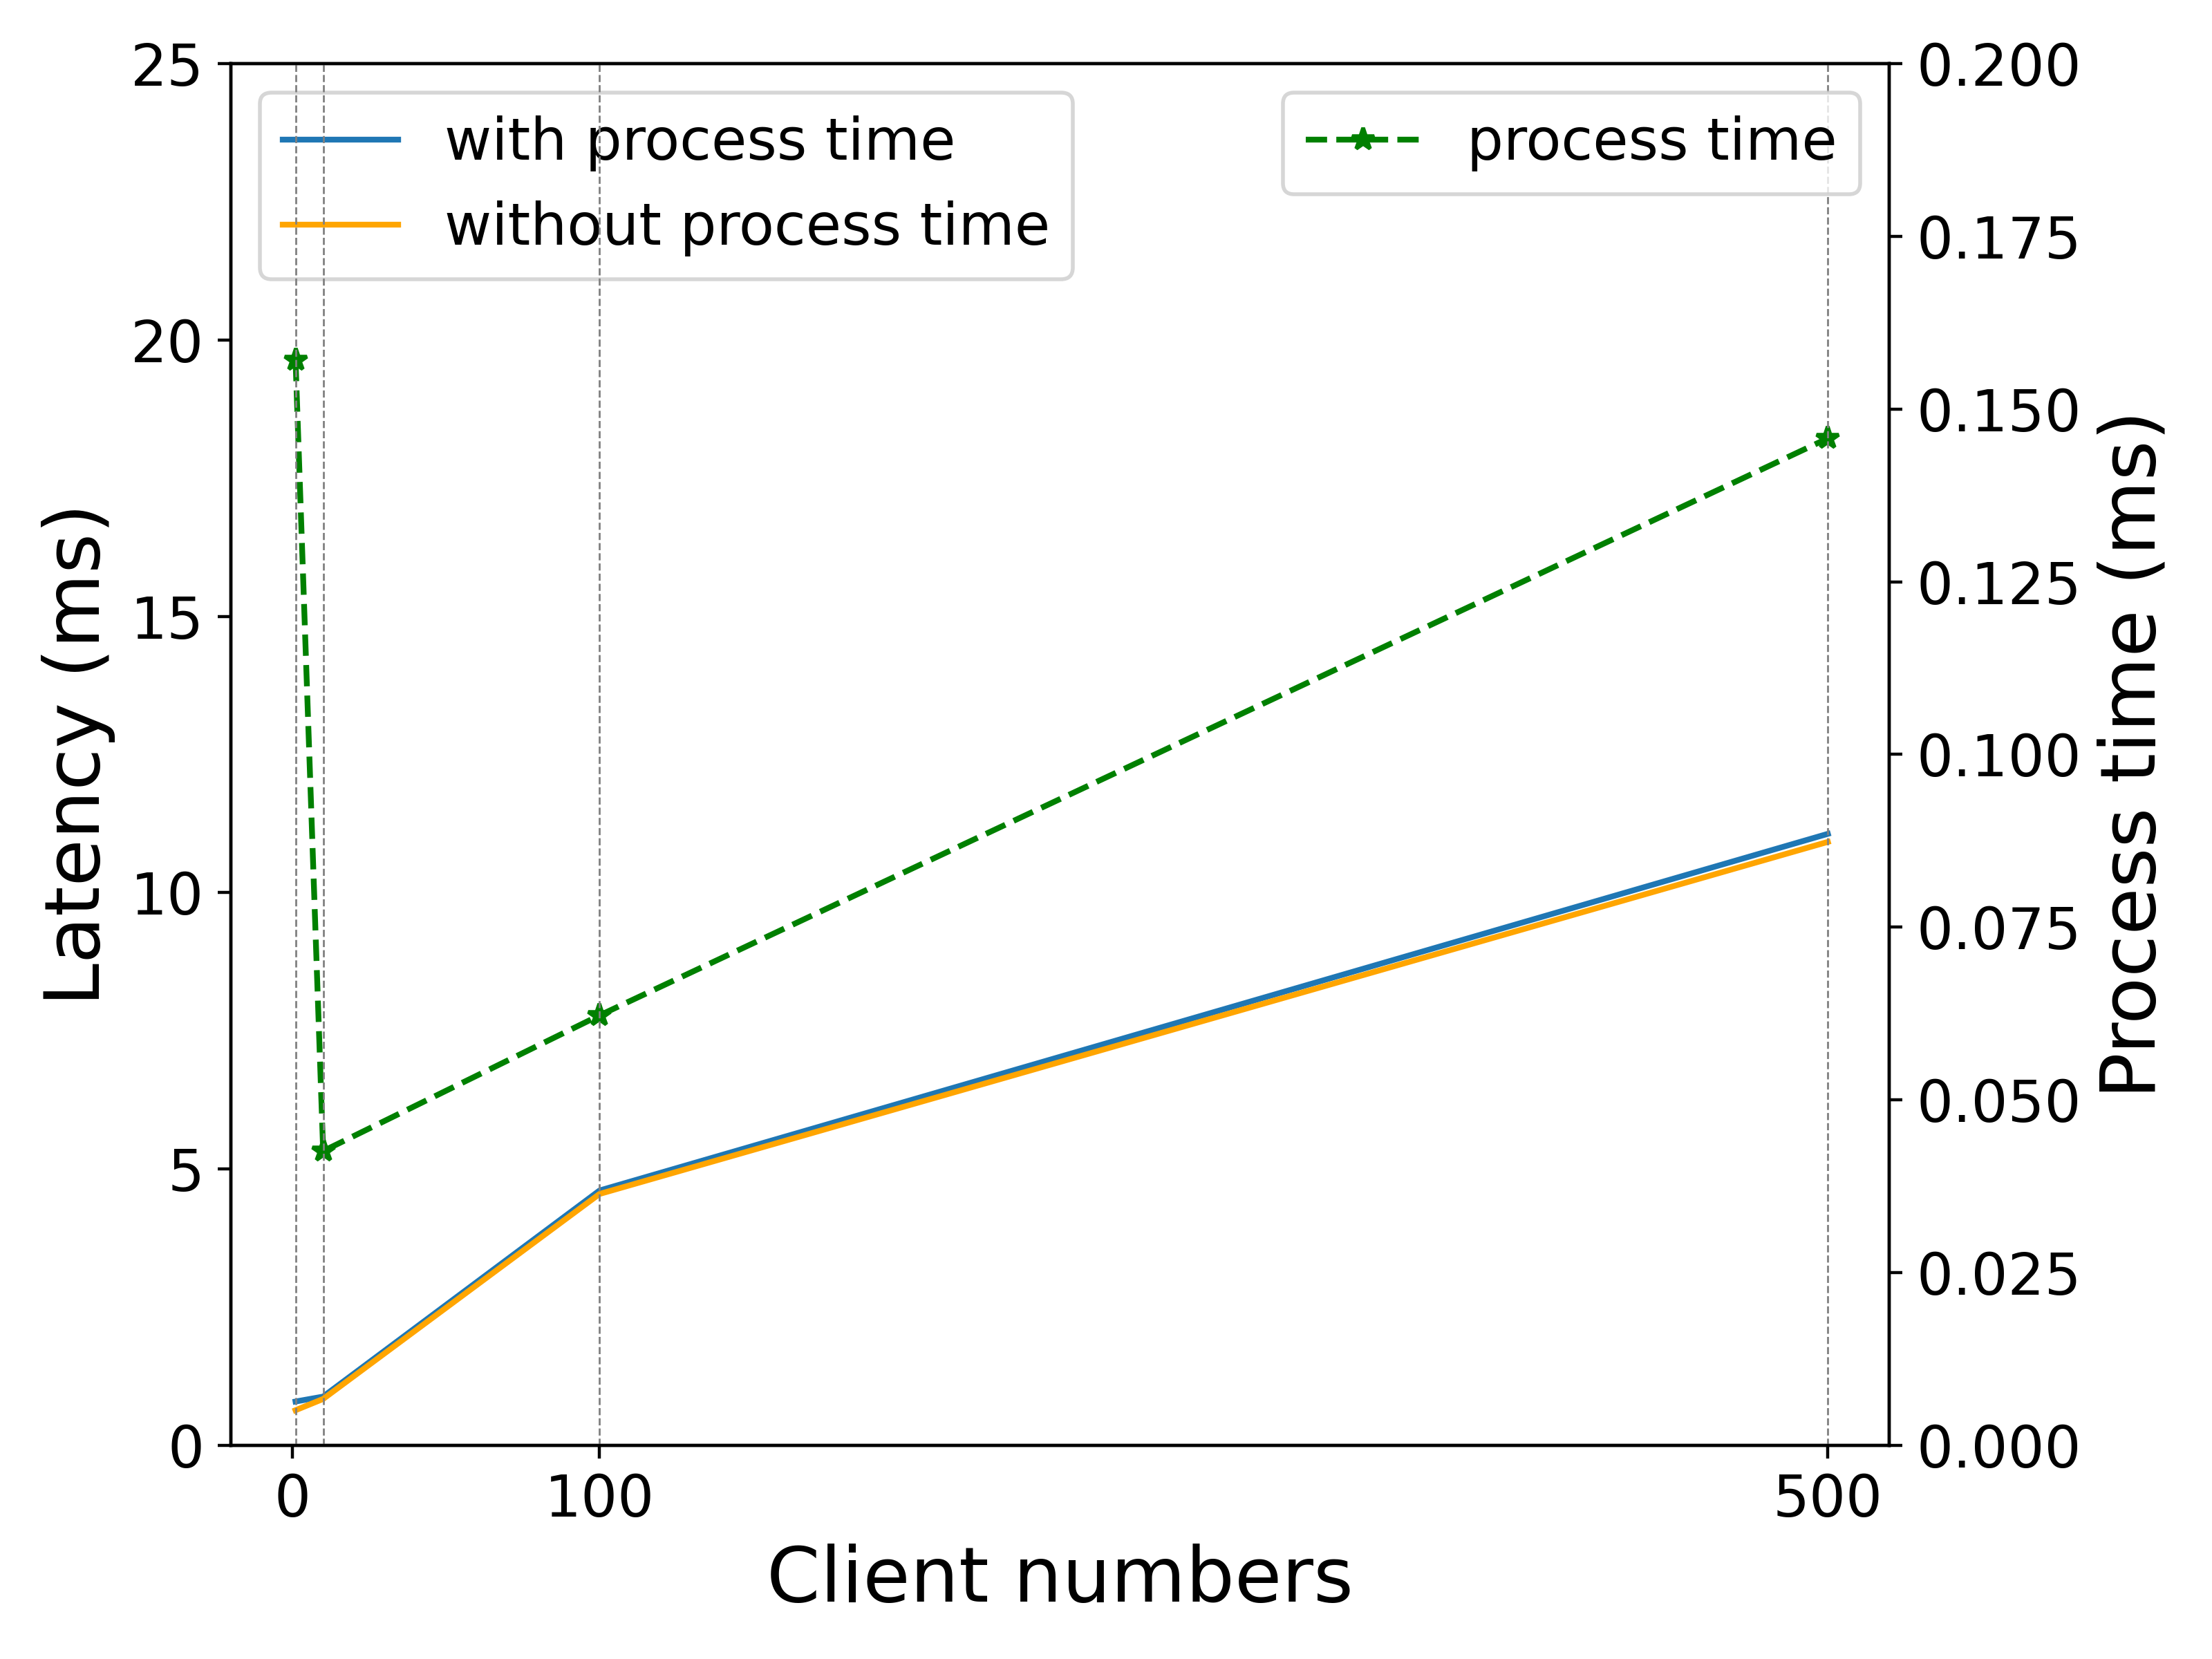
\includegraphics[width=\textwidth]{figures/tests/proportional_tests/Average_string_messages_sending_time_of_100_tests_of_diff_client_numbers.png}\hfill 
        \caption{} \label{fig: proportional-clients-a}
    \end{subfigure}
    \begin{subfigure}[b]{0.49\textwidth}
        \centering
        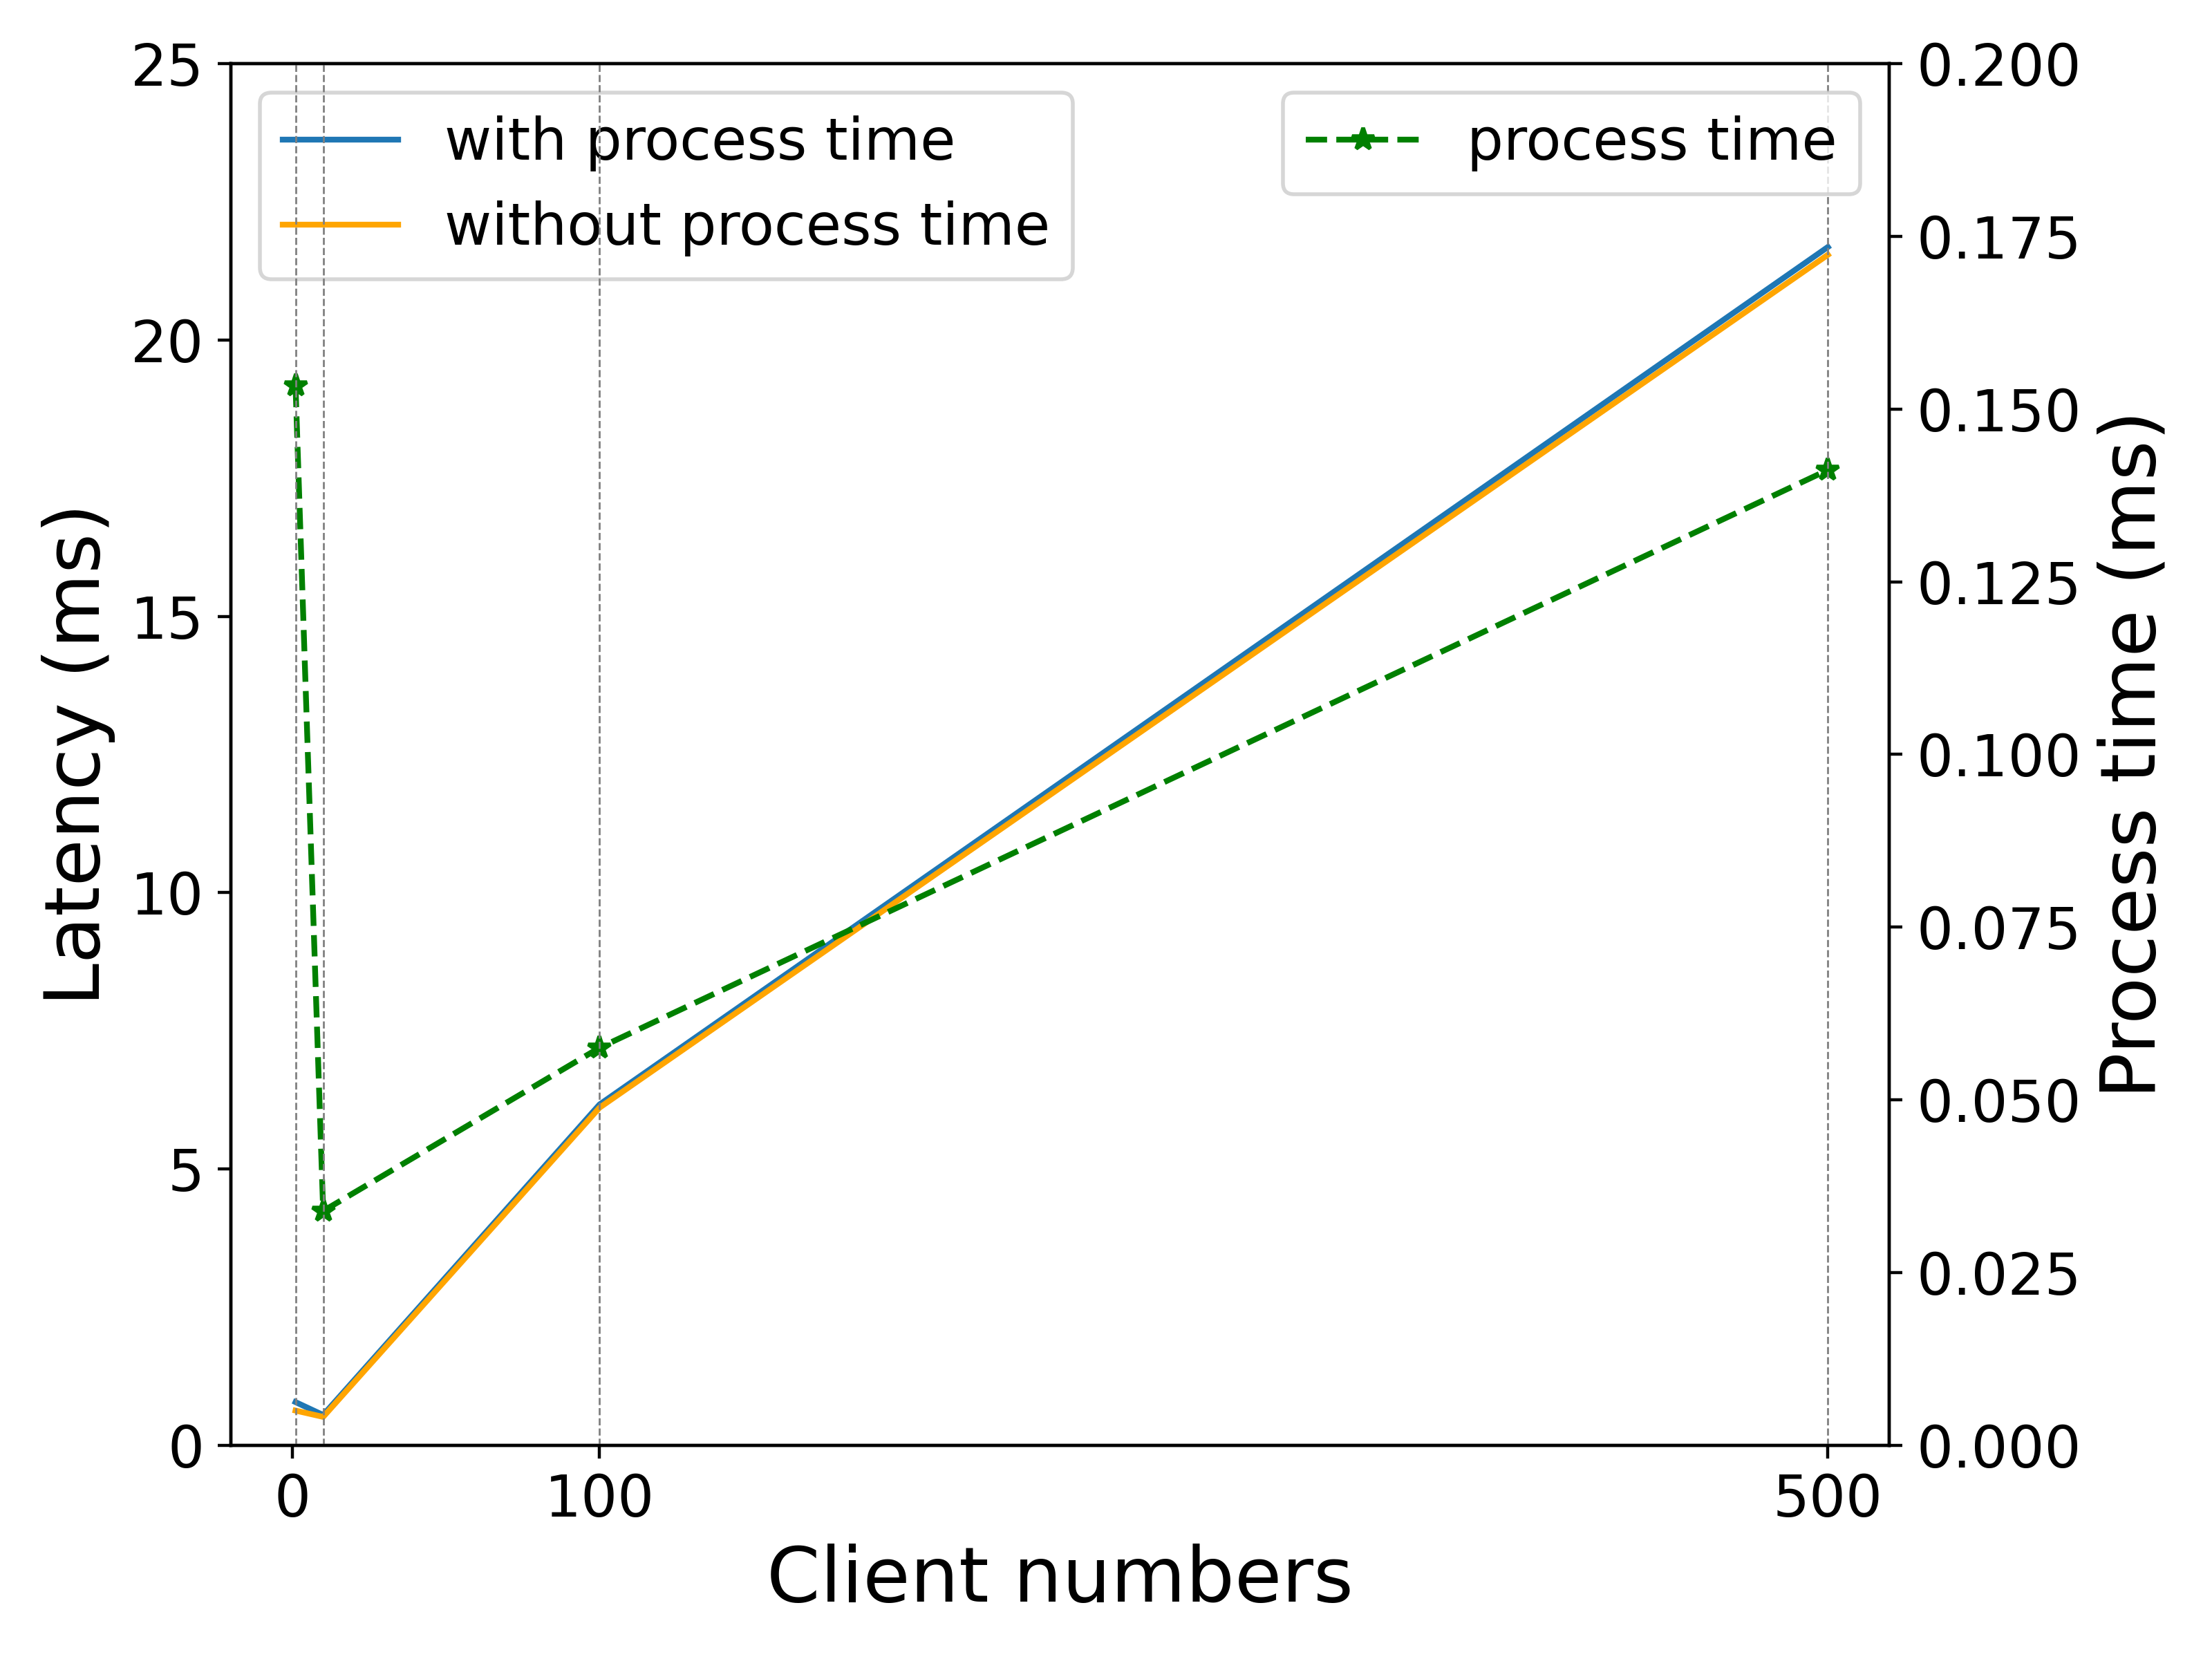
\includegraphics[width=\textwidth]{figures/tests/proportional_tests/Average_string_messages_receiving_time_of_100_tests_of_diff_client_numbers.png}\hfill 
        \caption{} \label{fig: proportional-clients-b}
        \end{subfigure}

    \caption{Average delay of sending a string message 100 times 
    to a clientR from 1, 10, 100 or 500 clients separately. (a) Messages sent forward, 
    and (b) response messages from clientR. 
    \label{fig: proportional-clients}}
\end{figure}


\subsubsection{Increasing server numbers}
When 1000 clients are communicating with clientR, their messages will be split 
into two or three groups and routed through different servers due to system 
limitations. According to fig.\ref{fig: NSConceptual}, only a maximum of three 
servers can be used for the test, as per the hardware configuration of the external 
routing solutions. However, we can make some assumptions based on the results 
shown in fig.\ref{fig: proportional-servers}.


\begin{figure}[htb]
    \centering
    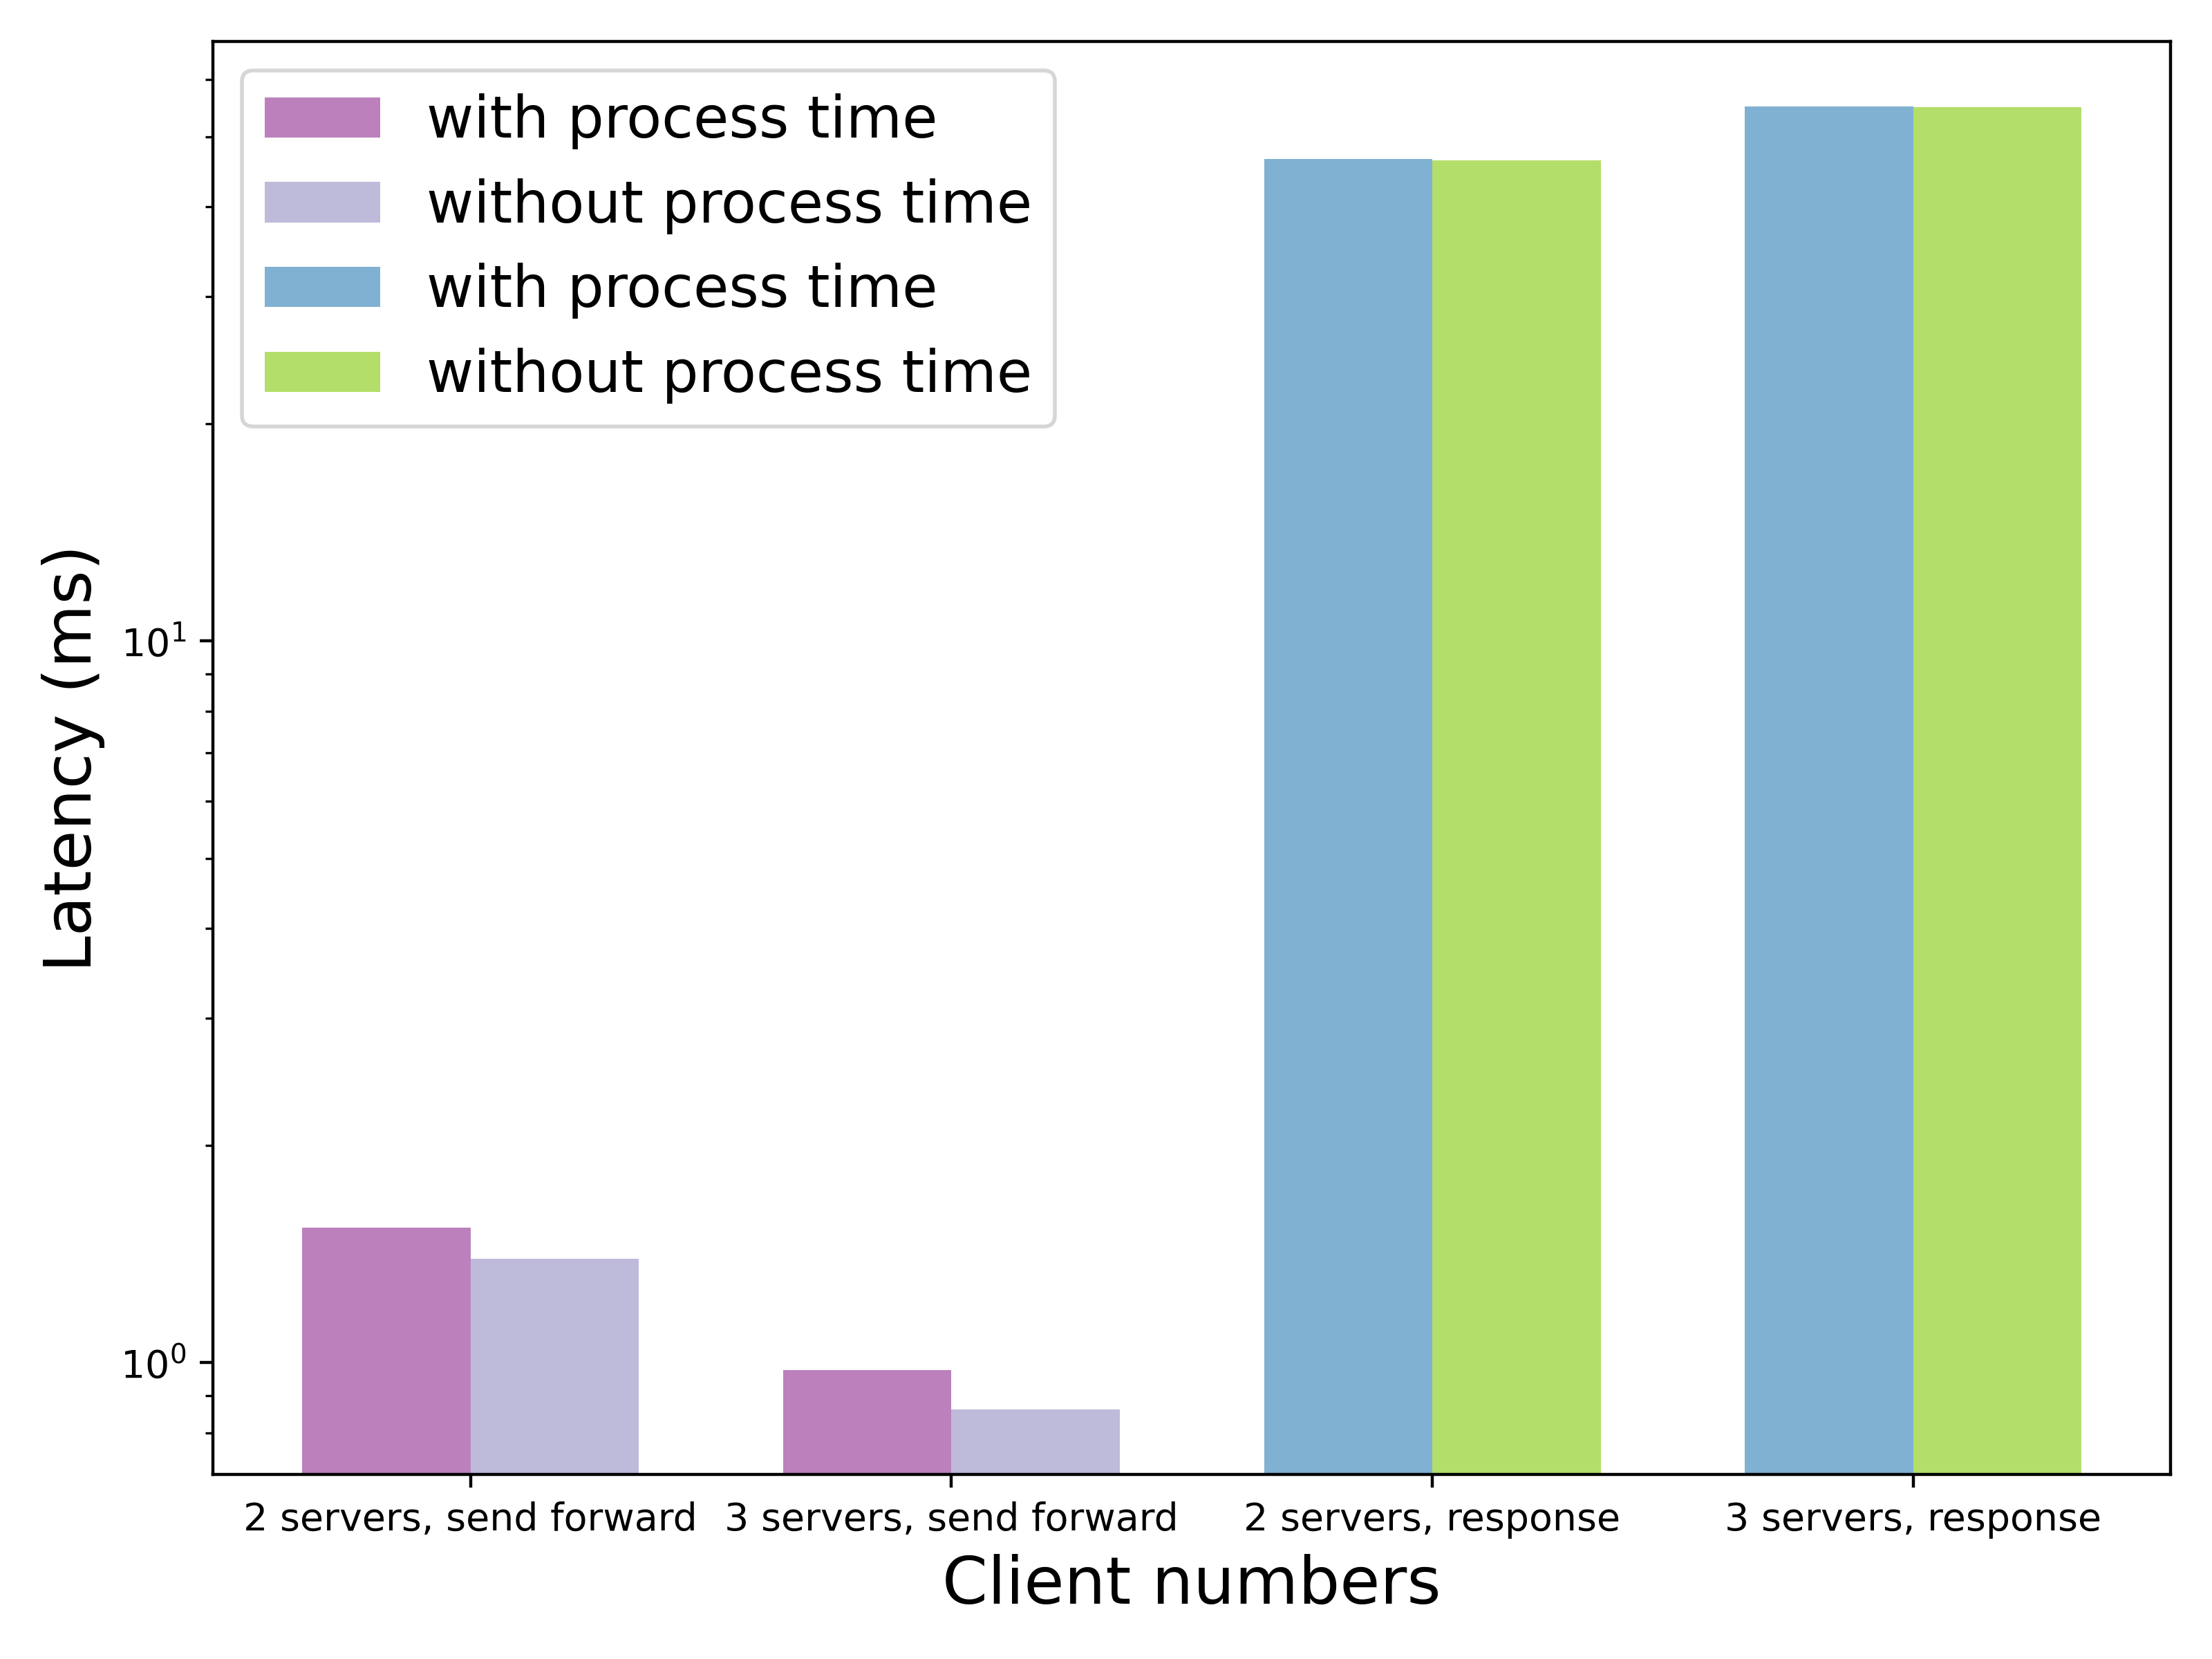
\includegraphics[width=0.8\textwidth]{figures/tests/proportional_tests/Average_string_messages_receiving_time_of_100_tests_diff_server_numbers.png}\hfill 
    \caption{Average delay of sending a string message 100 times 
    to a clientR from 1000 clients through 2 or 3 servers separately. 
    \label{fig: proportional-servers}}
\end{figure}

Fig.\ref{fig: proportional-servers} indicates that introducing 
additional servers to the system results in a reduction of latency. This means that 
limited productive resources can be better utilized for frequent client interactions. 
However, the latency of response messages from clientR is unexpectedly higher 
in fig.\ref{fig: proportional-servers}. This could be due to high \gls{cpu} consumption. 
When multiple servers are running on the same device, the send and receive processes 
in the WebSocket are operated separately. Due to the high occupation of \gls{cpu} power, 
the loads between each process might be unbalanced and added up by the increment of servers.

\subsubsection{Increasing string message length}\label{chap: Result-Internal-string}
To determine the effect of packet size (i.e., message length) on system performance, 
it is important to conduct another significant test. The 
formula\cite{forouzan2004data}\cite{kurose2005computer} for packet transmission 
time is given as:


\begin{equation}
    Transmission \; delay = Packet \; size/Bandwidth
\end{equation}

Assuming the bandwidth is constant, the transmission time should be linearly proportional 
to an increasing packet size. In fig.\ref{fig: proportional-stringsize}, various string 
message lengths ranging from 1KB to 10MB are compared, indicating the linear dependency 
of latency and string size in both forward (fig.\ref{fig: proportional-stringsize-a}) 
and return message (fig.\ref{fig: proportional-stringsize-b}). This confirms the 
transmission time formula. Additionally, it's worth noting that the server's process 
time increases with the size of the message bytes. In real-world scenarios, large string 
messages should be broken down into smaller parts for communication, significantly 
reducing process time consumption. To examine system limits, a string with a size of 
up to 100MB is tested, resulting in a system timeout error that exceeds the server's 
maximum processing capacity.

\begin{figure}[htb]
    \centering
    \begin{subfigure}{0.49\textwidth}
        \centering
        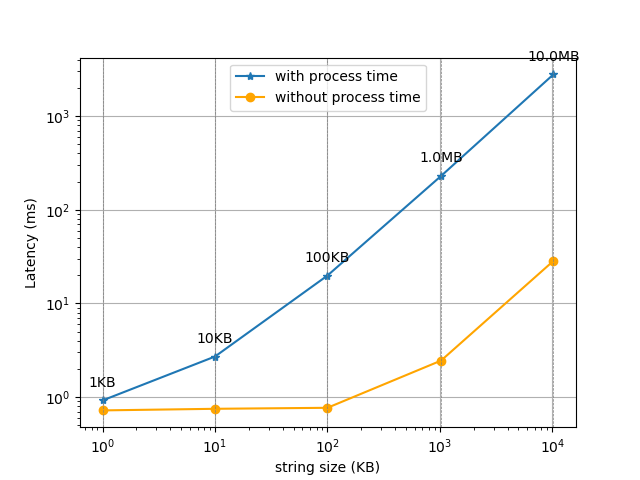
\includegraphics[width=\textwidth]{figures/tests/proportional_tests/log_Average_string_messages_sending_time_of_100_tests_1KB_to_10MB.png}
        \caption{} \label{fig: proportional-stringsize-c}
    \end{subfigure}
    \begin{subfigure}{0.49\textwidth}
        \centering
        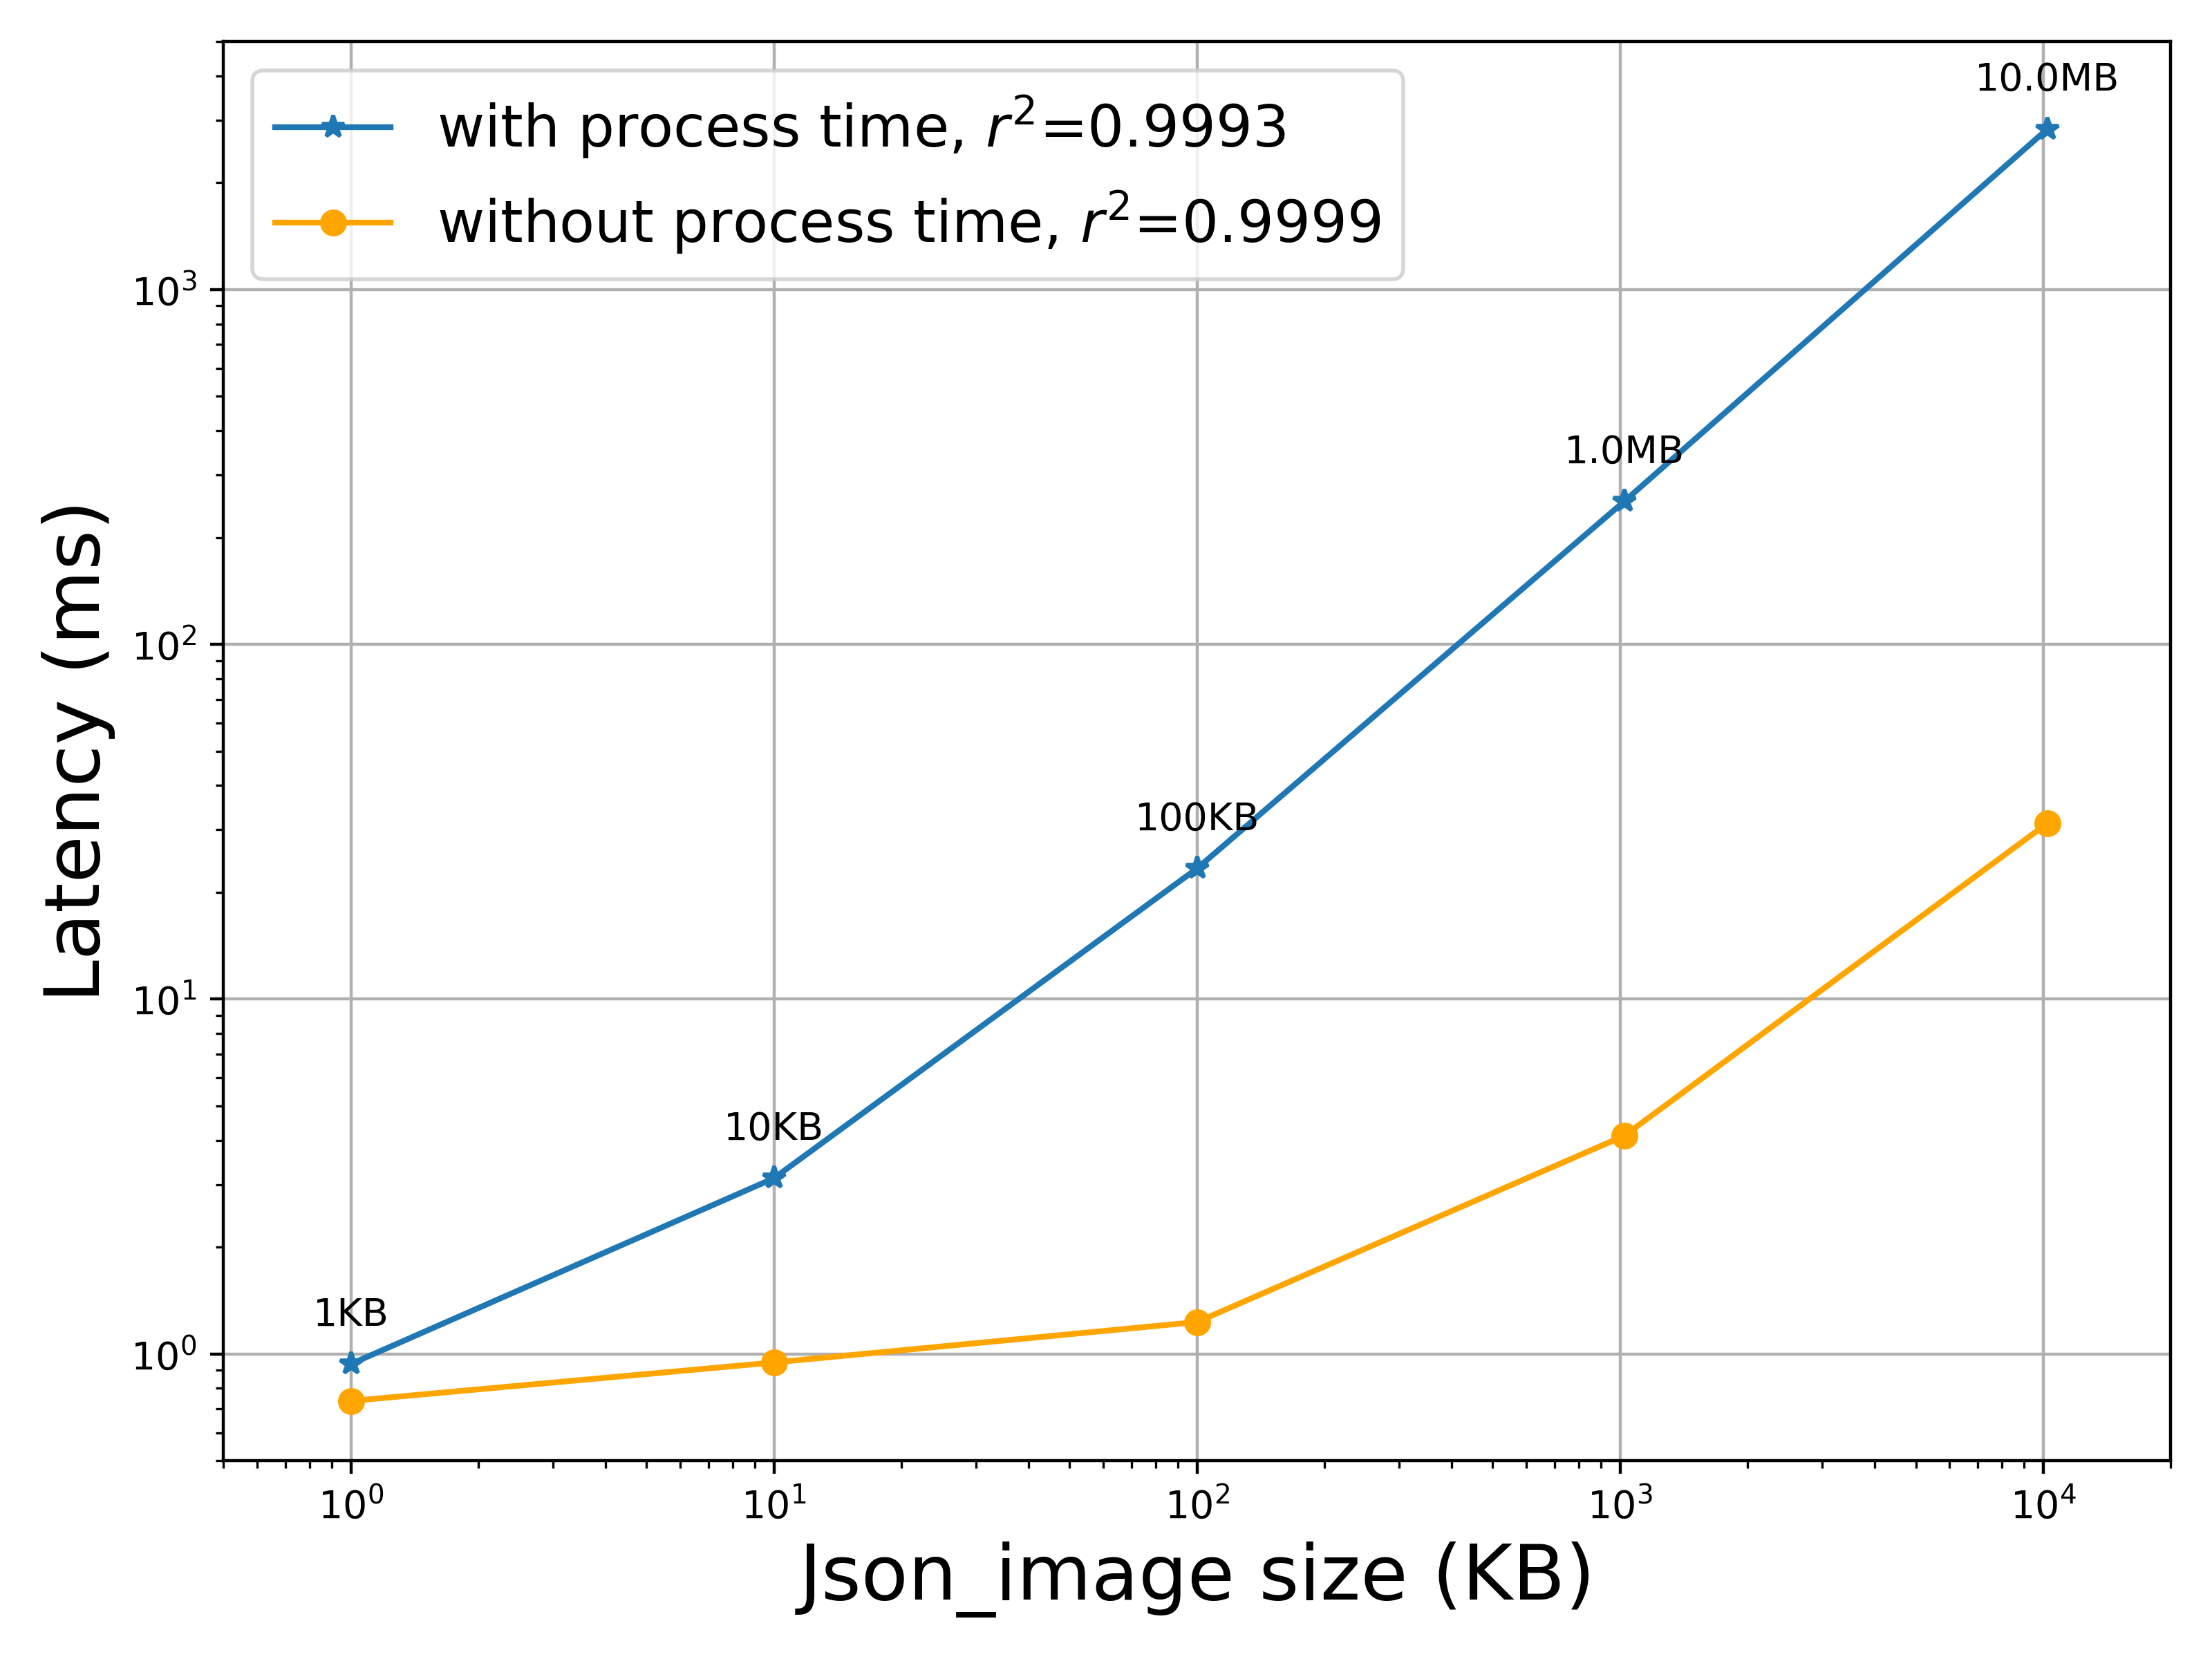
\includegraphics[width=\textwidth]{figures/tests/proportional_tests/log_Average_string_messages_receiving_time_of_100_tests_1KB_to_10MB.png}
        \caption{} \label{fig: proportional-stringsize-d}
    \end{subfigure}

    \begin{subfigure}{0.49\textwidth}
        \centering
        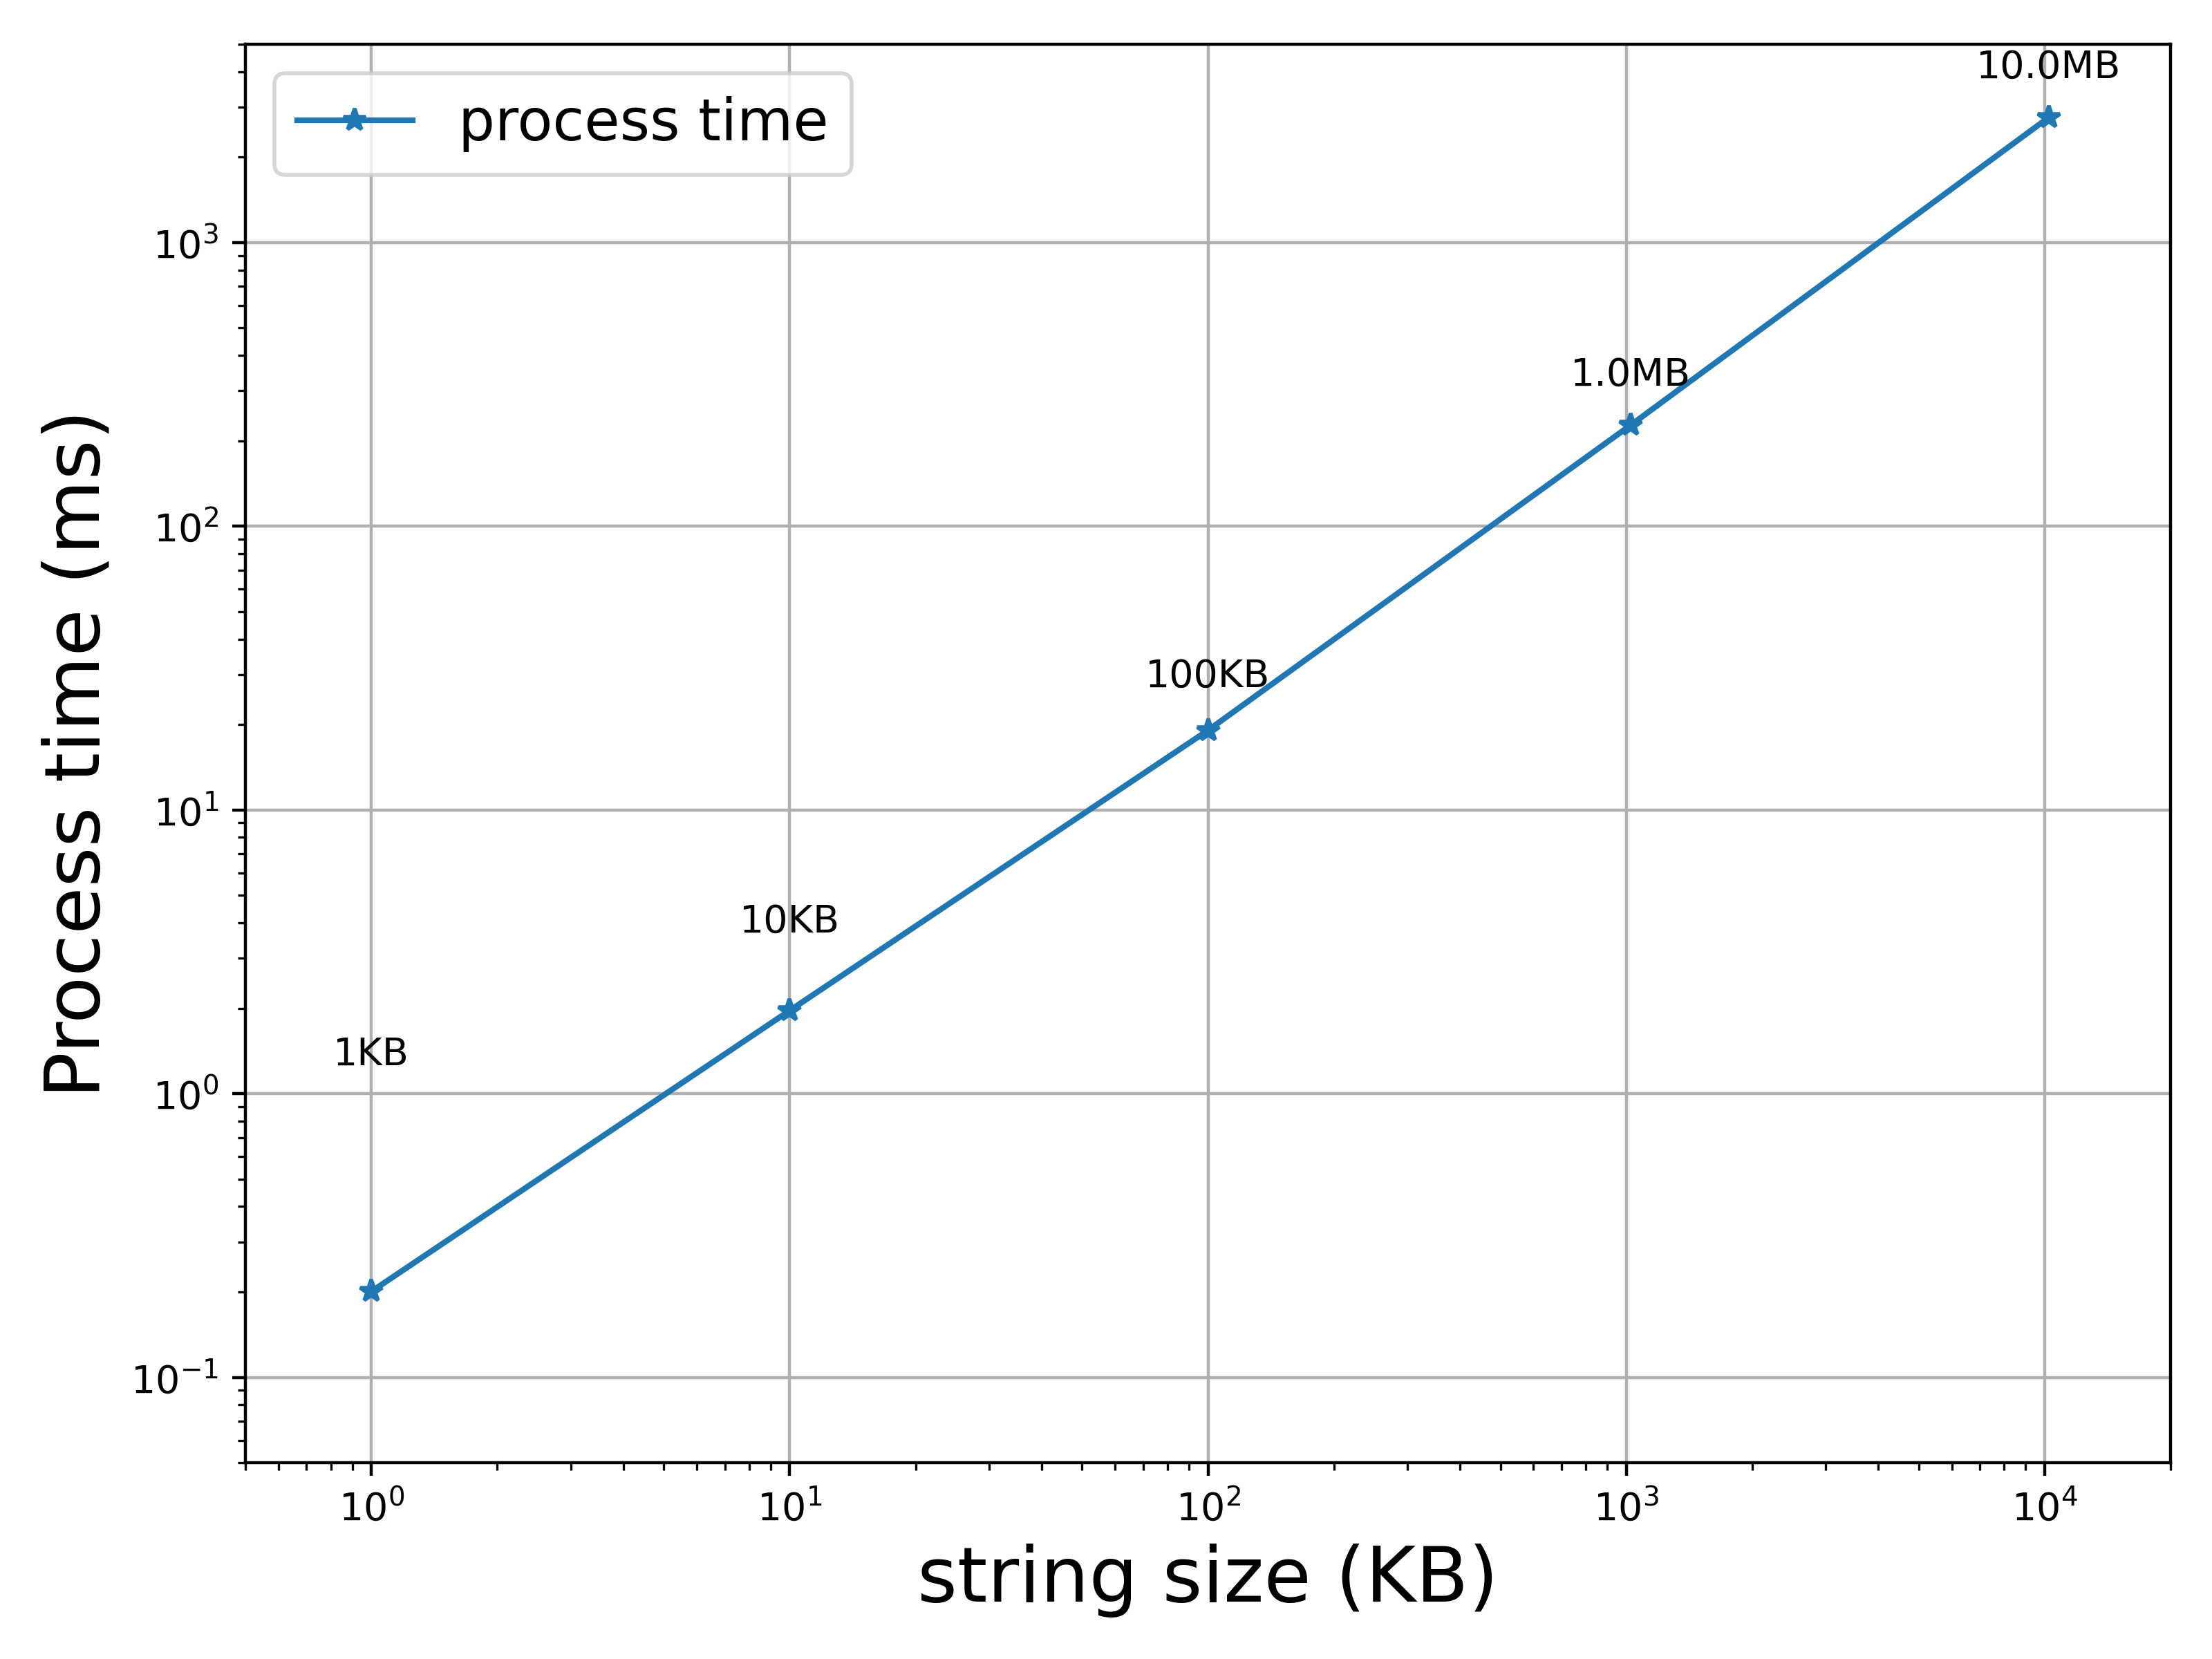
\includegraphics[width=\textwidth]{figures/tests/proportional_tests/Average_string_messages_sending_time_of_100_tests_1KB_to_10MB.png}
        \caption{} \label{fig: proportional-stringsize-a}
    \end{subfigure}
    \begin{subfigure}{0.49\textwidth}
        \centering
        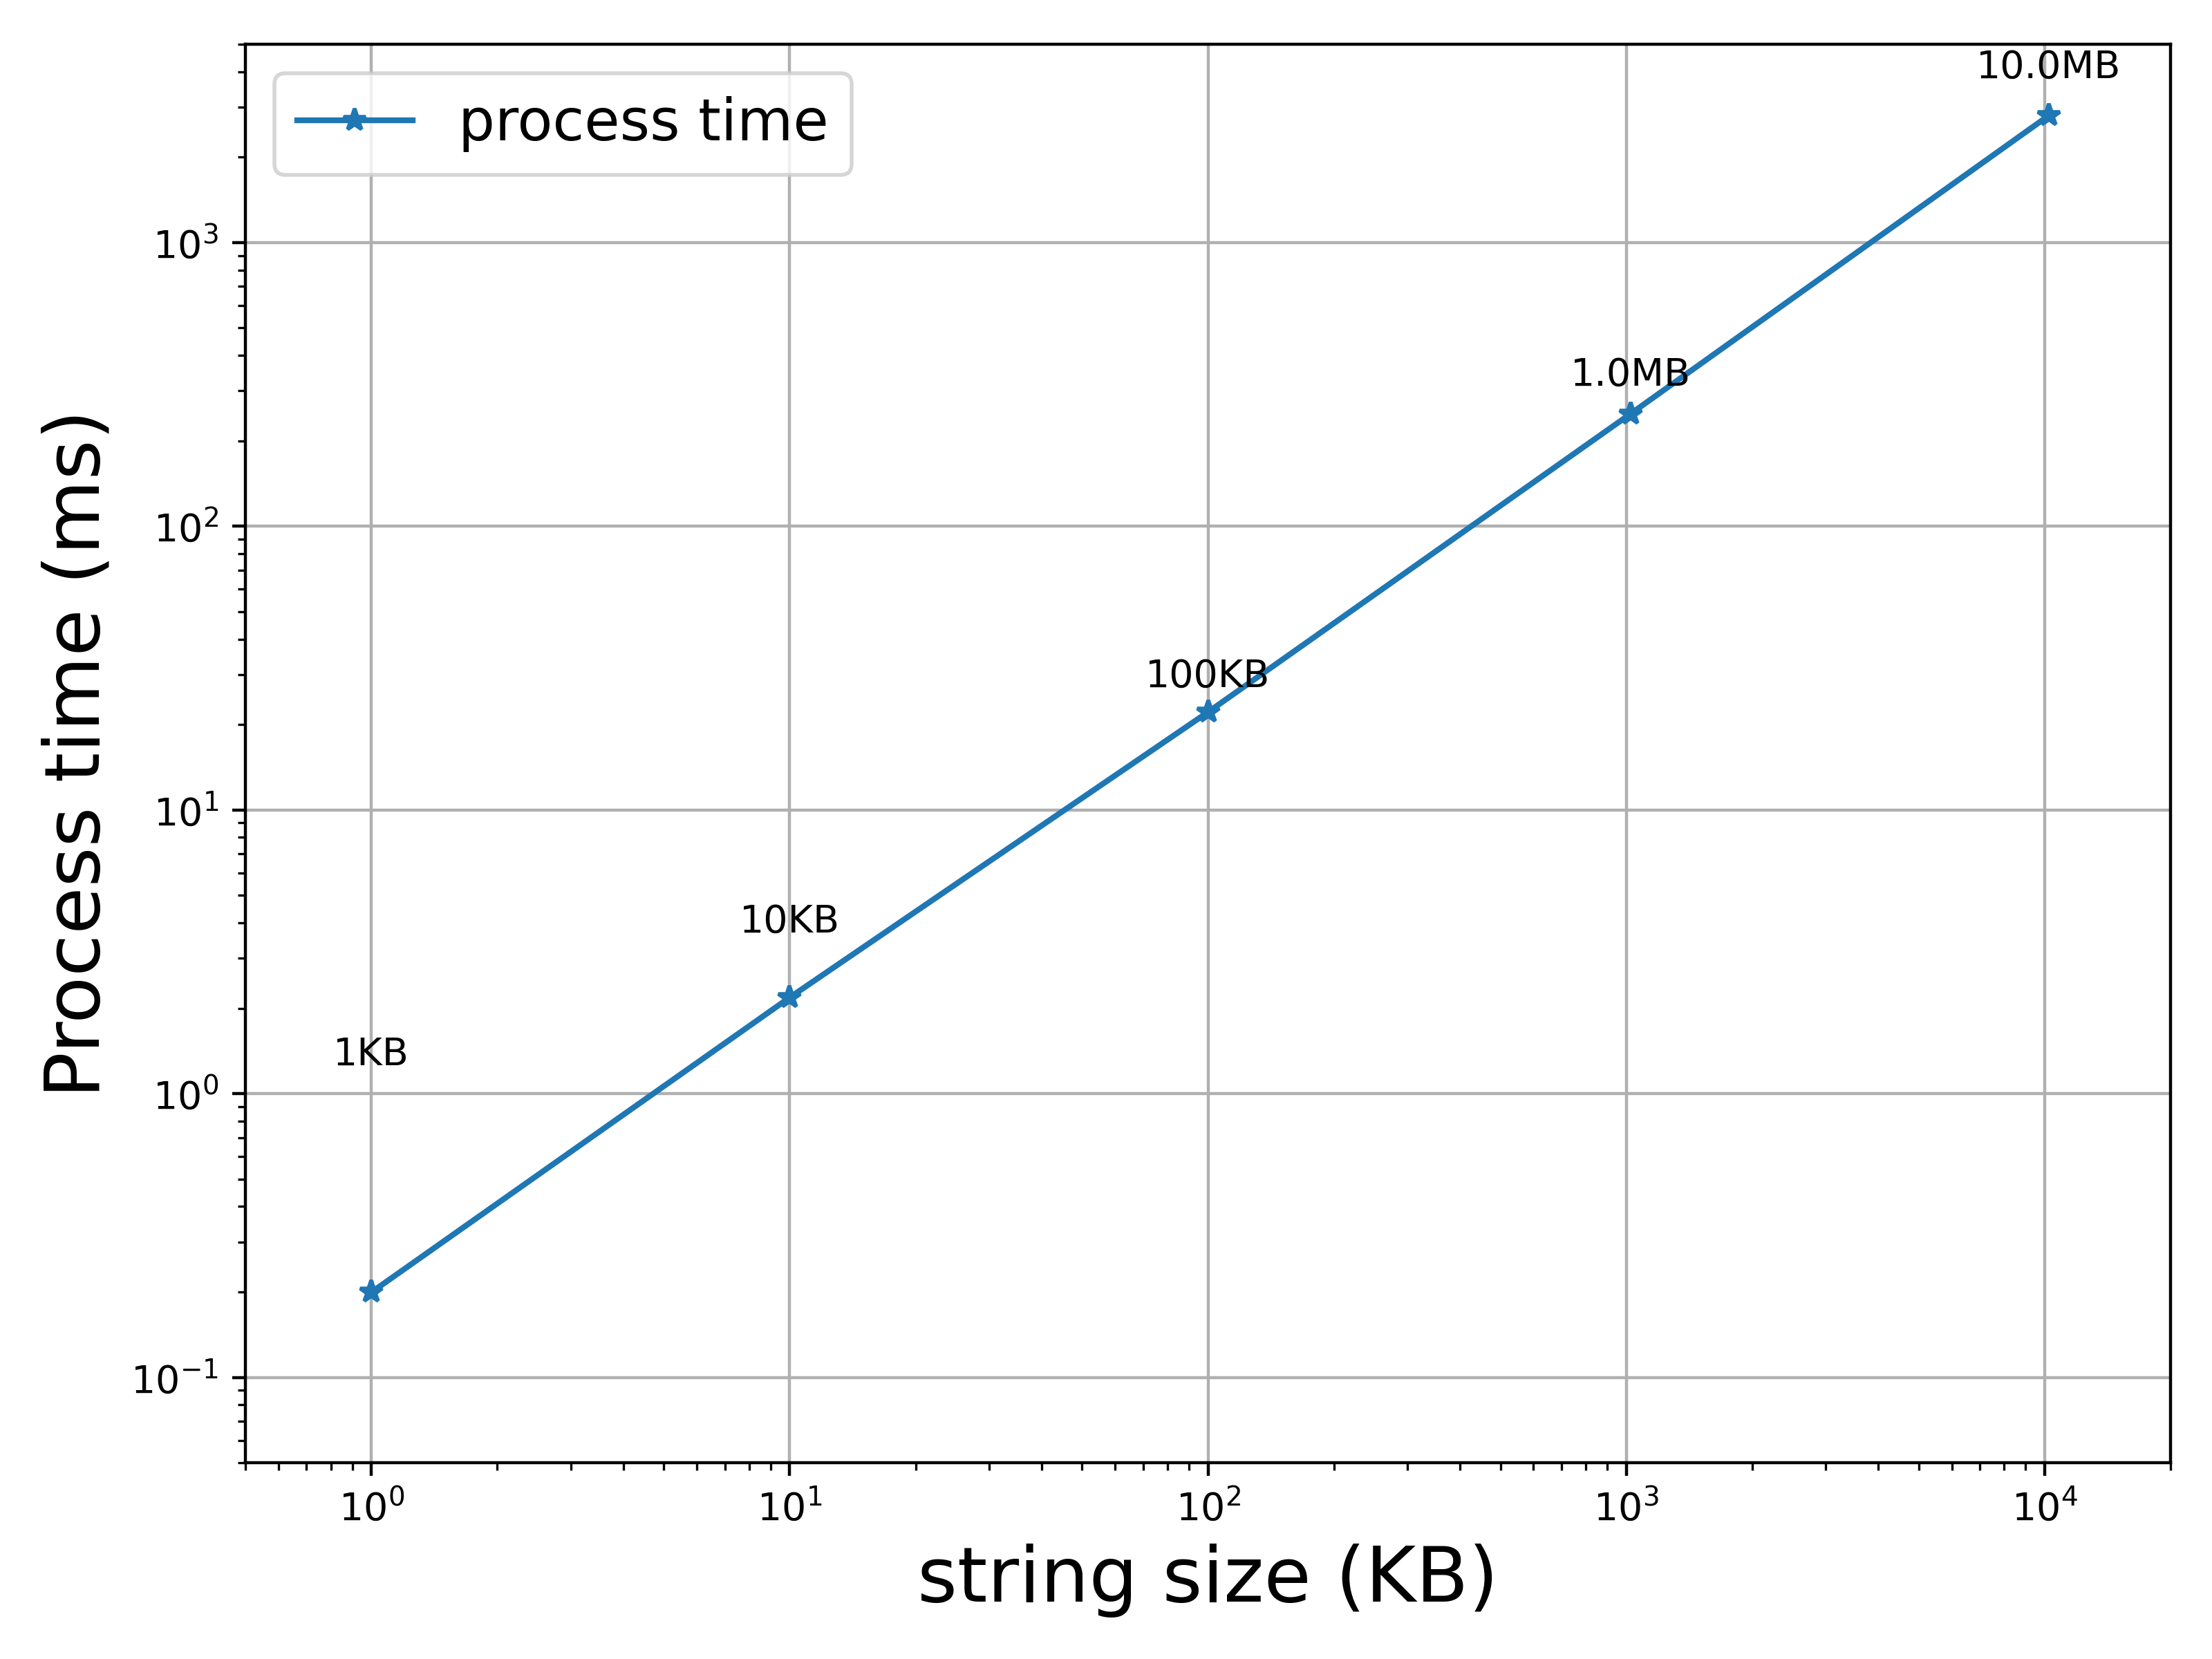
\includegraphics[width=\textwidth]{figures/tests/proportional_tests/Average_string_messages_receiving_time_of_100_tests_1KB_to_10MB.png} 
        \caption{} \label{fig: proportional-stringsize-b}
    \end{subfigure} 

    \caption{Average delay of sending and receiving a string message varied from 1KB 
    to 10MB for 100 times between 2 clients. (\subref{fig: proportional-stringsize-c}) Messages clientS sent forward, 
    (\subref{fig: proportional-stringsize-d}) response messages from clientR, 
    (\subref{fig: proportional-stringsize-a}) process time of massages sent forward 
    and (\subref{fig: proportional-stringsize-b}) process time of massages respond. 
    \label{fig: proportional-stringsize}}
\end{figure}

\subsubsection{Increasing JSON message length}
In addition to string, images are also frequently transported between different agents. 
However, unlike string messages, image sizes can be significantly larger, even up to over 
100MB for raw images. In addition, the agent's ID or message priority information should 
also be included in the message. Therefore, to send an image, it should be jsonified with 
the necessary information and then sent to the server. 



The tests for images are similar to those for string messages, with image size varying 
from 1KB to 100MB. Fig.\ref{fig: proportional-imagesize-a} and \ref{fig: proportional-imagesize-b} 
show the linear dependency of latency and jsonified image size. Although the transmission 
time for 1KB to 10MB messages is similar to the string test, there is a significant 
difference in process time between them. Comparing fig.\ref{fig: proportional-stringsize-c} 
with \ref{fig: proportional-imagesize-c} and fig.\ref{fig: proportional-stringsize-d} 
with \ref{fig: proportional-imagesize-d}, it is clear that the server process time for 
string messages is much higher than that for image messages. Moreover, due to the 
additional overhead of the JSON format, the network delay of string messages is 
relatively minor compared to that of image messages. 




One possible reason for the longer process time for string messages is that the server 
ust process them twice: once to split the message to extract the client ID, and again 
to recombine it for further transport. On the other hand, a jsonified image will only 
be processed once to extract the client information, and the original JSON file will 
be further transported directly.



\begin{figure}[htb]
        \centering
    \begin{subfigure}{0.49\textwidth}
        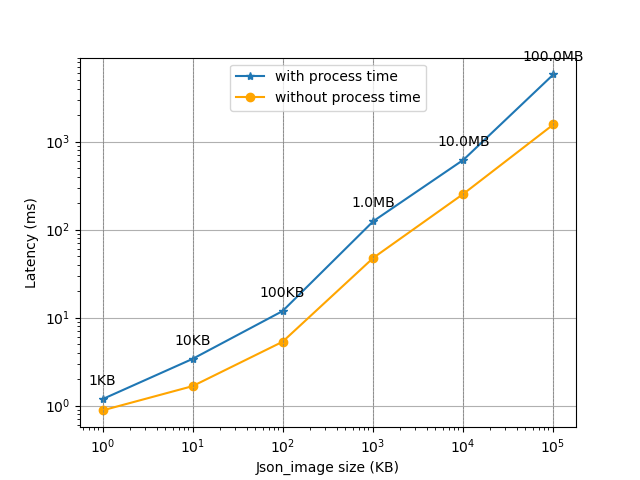
\includegraphics[width=\textwidth]{figures/tests/proportional_tests/log_Average_json_image_messages_sending_time_of_100_tests_1KB_to_100MB.png}\hfill 
        \caption{} \label{fig: proportional-imagesize-c}
    \end{subfigure}
    \begin{subfigure}{0.49\textwidth}
        \centering
        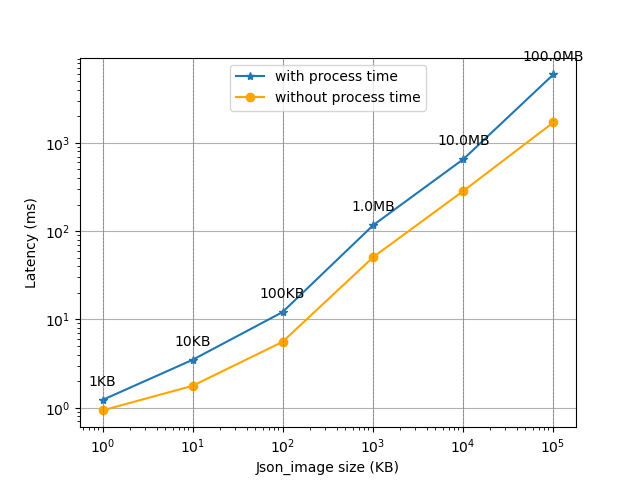
\includegraphics[width=\textwidth]{figures/tests/proportional_tests/log_Average_json_image_messages_receiving_time_of_100_tests_1KB_to_100MB.png}\hfill 
        \caption{} \label{fig: proportional-imagesize-d}
    \end{subfigure}
    \begin{subfigure}{0.49\textwidth}
        \centering
        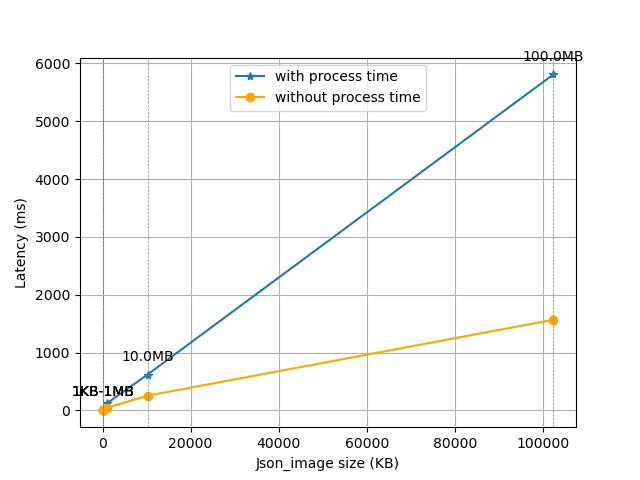
\includegraphics[width=\textwidth]{figures/tests/proportional_tests/Average_json_image_messages_sending_time_of_100_tests_1KB_to_100MB.png}\hfill 
        \caption{} \label{fig: proportional-imagesize-a}
    \end{subfigure}
    \begin{subfigure}{0.49\textwidth}
        \centering
        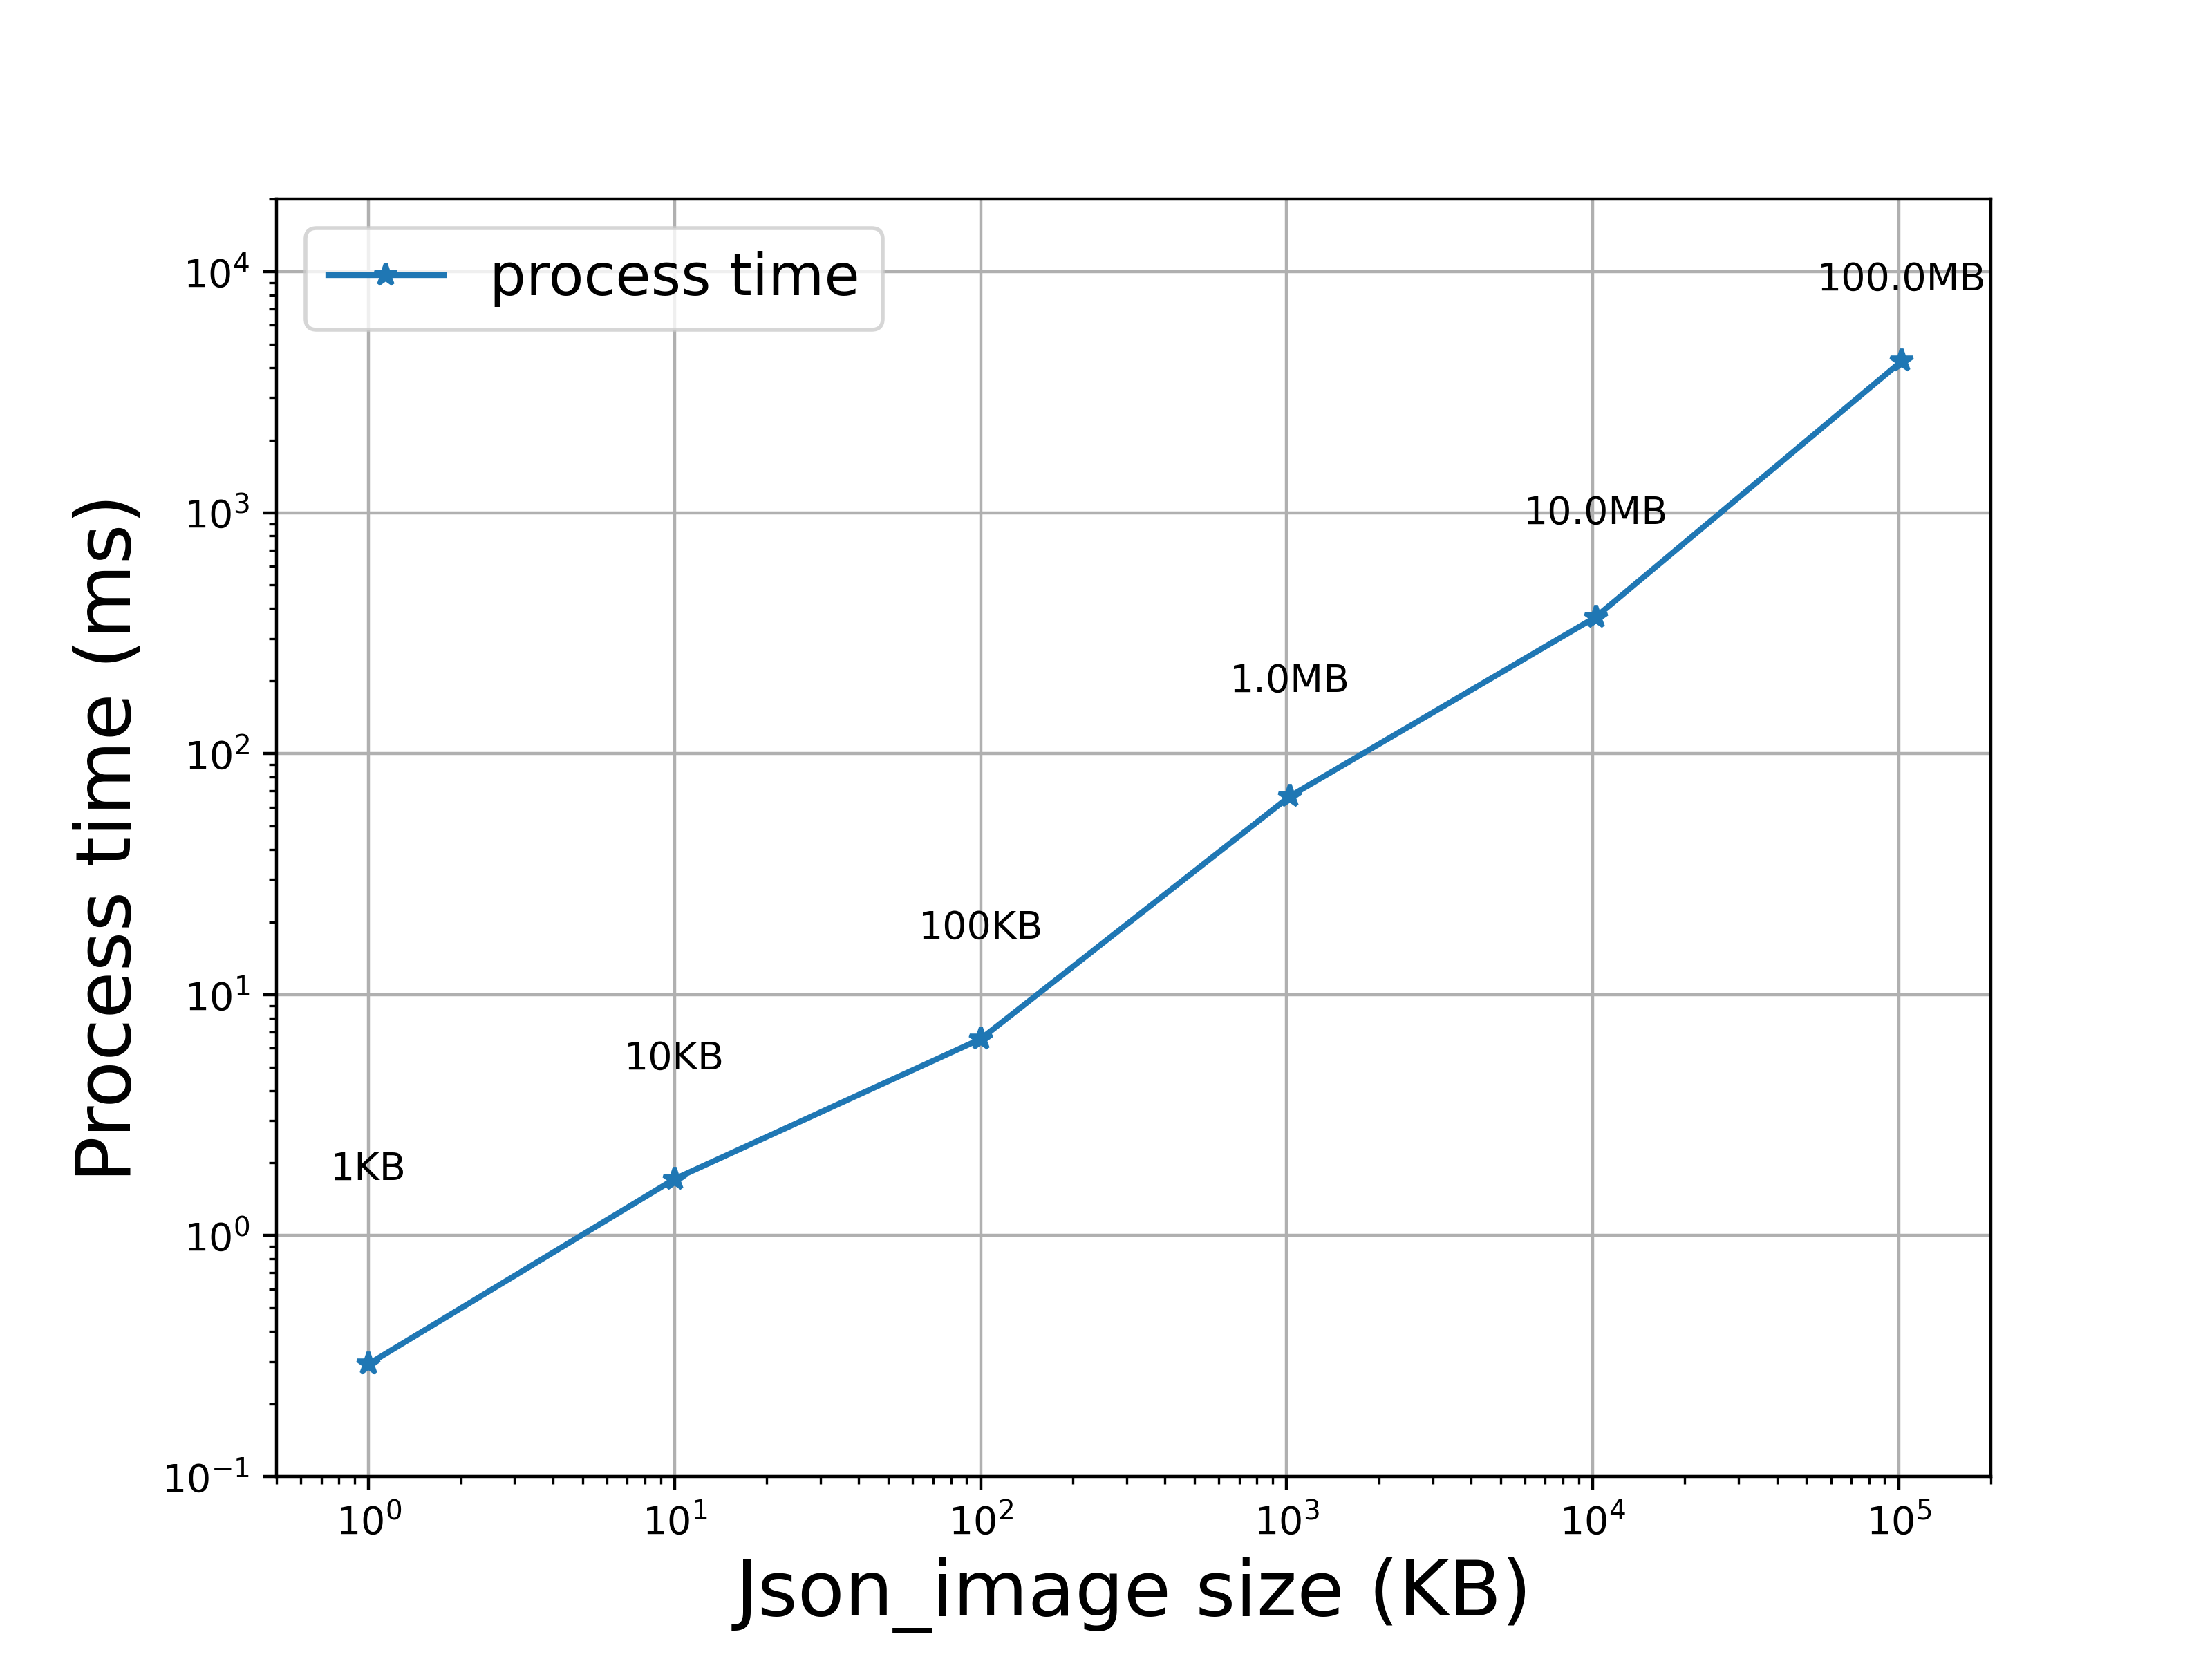
\includegraphics[width=\textwidth]{figures/tests/proportional_tests/Average_json_image_messages_receiving_time_of_100_tests_1KB_to_100MB.png}\hfill 
        \caption{} \label{fig: proportional-imagesize-b}
    \end{subfigure}

    \caption{Average delay of sending and receiving a jsonified image message varied from 1KB 
    to 100MB for 100 times between 2 clients. (\subref{fig: proportional-imagesize-c}) 
    Messages clientS sent forward in log form, 
    (\subref{fig: proportional-imagesize-d}) response messages from clientR in log form, 
    (\subref{fig: proportional-imagesize-a}) process time of messages sent forward  
    and (\subref{fig: proportional-imagesize-b}) process time of response messages from clientR. 
    \label{fig: proportional-imagesize}}
\end{figure}

\subsection{Pseudocode of one-to-one agent communication workflow in RESTful API}\label{chap: Meth-REST-pseudocode}
A more comparable application layer protocol is \gls{http}, which has the request-response mechanism with more additional functionalities compared to \gls{http}. 
Therefore, \gls{http} was considered an alternative communication protocol other 
than WebSocket. 
Different from WebSocket, the design of \gls{http} based system is 
only built for performance testing and its results will be compared to those from 
WebSocket. In the pseudocode 
below, RESTful API will be used as a Web Service API, an interface to connect 
two devices over the internet based on \gls{http} protocol. With the design 
based on RESTful API, the clients can communicate with each other by using its 
standard \gls{crud} operations, for example, POST and GET, to send and receive 
messages. 
Therefore, the RESTful API system is simplified to one-to-one agent communication 
without other functionalities like decision-making or message prioritization, 
among others.


According to the pseudo-code for agentS (send and receive messages) and agentR (receive and send messages) in algorithm \ref{alg: SRPseudoCode} and \ref{alg: RSPseudoCode}, and the server in algorithm \ref{alg: apiServerPseudoCode}, the primary mechanism is similar to the one designed for WebSocket. One significant difference is that the connection will be closed after the message is sent from the clientS to clientR. If the agentR needs to send a response message back to inform the success, re-connection is needed. 
Instead of sending and receiving from WebSocket, agentS first POST a request to the server to call the function $send\_message()$, 
while agentR GET a request to the server for the function call $get\_message()$, same for the reverse direction. 
Under the same condition, the message transport routine with RESTful API may result in more latency than WebSocket, which will be verified later.


\begin{algorithm}
    \caption{Pseudocode for agentS in one to one communication workflow.}
    \label{alg: SRPseudoCode}
    \begin{algorithmic}[1]
    \State {Import} flask
    \State {Initialize} agentID, serverIP
        \State \textbf{function} {$send\_and\_receive(sender, recipient, msg)$}
        \State \qquad format msg with agent IDs 
        \State \qquad post request msg to server
        \State \textbf{\qquad while} no response \textbf{do}    
        \State \qquad \qquad {$wait\_for\_response(sender, recipient)$}

        \State \textbf{function} {$wait\_for\_response(sender, recipient)$}
        \State \textbf{\qquad while} message not received \textbf{do}    
        \State \qquad \qquad get request jsonMsg from server and wait for reponse
        \State \qquad \qquad parse jsonMsg to retrieve message content
    

    \State \textbf{Main:}
    \State \qquad {$send\_and\_receive(agentID, recipient, msg)$}
    \State \textbf{End} 
    \end{algorithmic}
\end{algorithm}


\begin{algorithm}
    \caption{Pseudocode for agentR in one to one communication workflow.}
    \label{alg: RSPseudoCode}
    \begin{algorithmic}[1]
    \State {Import} flask
    \State {Initialize} agentID, serverIP
        \State \textbf{function} {$send\_message(recipient, msg)$}
        \State \qquad format msg with recipient ID 
        \State \qquad post request msg to server and wait for response 

        \State \textbf{function} {$get\_message(agentID)$}  
        \State \qquad get request jsonMsg from server and wait for response
        \State \qquad parse jsonMsg to retrieve message content
        \State \qquad \textbf{return} msg, recipient         

    \State \textbf{Main:}
    \State \qquad {$msg, recipient = get\_message(agentID)$}
    \State \textbf{\qquad if} msg AND recipient \textbf{then}   
    \State \qquad \qquad{$send\_message(recipient, msg)$}
    \State \textbf{End} 
    \end{algorithmic}
    \end{algorithm}

\begin{algorithm}
    \caption{Pseudocode for a server in one to one communication workflow.}
    \label{alg: apiServerPseudoCode}
    \begin{algorithmic}[1]
    \State {Import} flask
    \State {Initialize} jsonMsg 
    \State \textbf{Class} app
        \State \qquad \textbf{function} {$send\_message()$}
        \State \qquad \qquad {\# POST request in app class} 
        \State \qquad \qquad parse the json file from request
        \State \qquad \qquad retrieve recipient and message content 
        \State \qquad \qquad \textbf{if} recipient AND msgContent \textbf{then}
        \State \qquad \qquad \qquad jsonify senderIP and message content and store in jsonMsg
        \State \qquad \qquad \qquad response is OK status code
        \State \qquad \qquad \textbf{else}            
        \State \qquad \qquad \qquad response is Error code            
        \State \qquad \qquad \textbf{return} response  

        \State \qquad \textbf{function} {$get\_message(agentID)$}  
        \State \qquad \qquad {\# GET request in app class} 
        \State \qquad \qquad \textbf{if} agentID in jsonMsg \textbf{then}
        \State \qquad \qquad \qquad send jsonMsg and response is OK status code
        \State \qquad \qquad \textbf{else}
        \State \qquad \qquad \qquad response is Error code
        \State \qquad \qquad \textbf{return} response         

    \State \textbf{Main:}
    \State \qquad Instantiate app
    \State \qquad run app forever
    \State \textbf{End} 
    \end{algorithmic}
    \end{algorithm}

\subsection{Test results of WebSocket and \gls{http}} \label{chap: Result-RestFUL_WS}
After testing the performance of the WebSocket-based communication system, it will be 
interesting to see whether the other application layer protocols with different message 
transport mechanisms will have a similar or completely different performance under the 
same conditions between two clients. As demonstrated from fig.\ref{fig: MsgConceptual}, \gls{http} is designed 
for message transport in both directions and, therefore, more comparable with WebSocket 
among the others. As a result, a \gls{http} based interface RESTful API is designed under 
a similar architecture as WebSocket and tested under the exact condition of the WebSocket 
string test in section \ref{chap: Result-Internal-string}. By comparing 
fig.\ref{fig: proportional-stringsize} with fig.\ref{fig: proportional-rest-stringsize}, 
it is evident that the processing time of string messages is higher and grows faster in 
a WebSocket server than in a RESTful API server. The difference may result in the 
prioritization and data processing mechanisms in the WebSocket server. In contrast, 
the RESTful API server is only designed with a simple message POST and GET mechanism. 
However, the data transmission time between both is more comparable. First of all, 
both of them reflect the fit of the model with the coefficient of determination close 
to one, which is namely\cite{archdeacon1994correlation}: 


    \begin{align}
        R^{2} &= 1-\frac{RSS}{TSS}\\
        \text{Where} \nonumber\\
        RSS & = \text{sum of squared residuals} \nonumber\\
        TSS & = \text{total sum of squares}\nonumber
    \end{align}

meaning that the model fits the data well (considered a good fit for $R^{2}>0.7$).





Secondly, the transmission time of both is similar 
for the same string message length (RESTful has slightly higher latency), with a difference 
of 0.01ms to a few milliseconds, which grows over message size. 



Therefore, WebSocket is proven more appropriate for real-time message transport, 
essential for an agent-based system. However, an ignorable data process time for \gls{mqtt} 
indicates that, a lightweight \gls{mqtt} could be more appropriate for simple data 
transmission tasks.


\begin{figure}[htb]
    \begin{subfigure}[b]{0.49\textwidth}
        \centering
        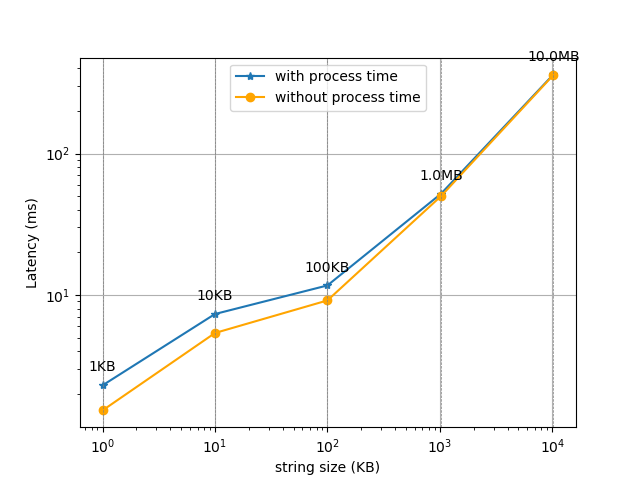
\includegraphics[width=\textwidth]{figures/tests/proportional_tests/Rest_log_Average_string_messages_sending_time_of_100_tests.png}\hfill 
        \caption{} \label{fig: proportional-rest-stringsize-c}
    \end{subfigure}
    \begin{subfigure}[b]{0.49\textwidth}
        \centering
        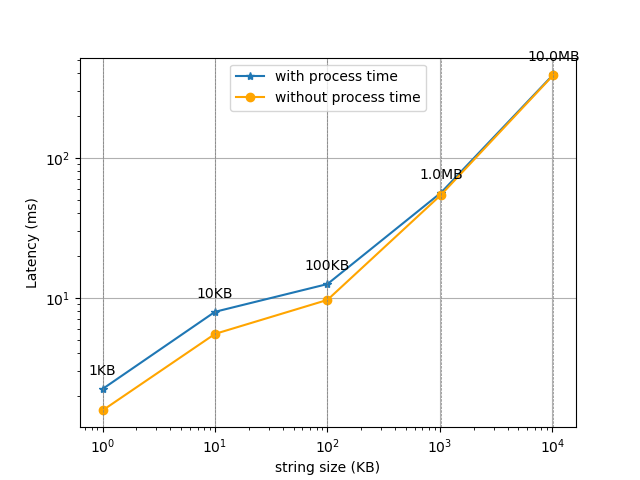
\includegraphics[width=\textwidth]{figures/tests/proportional_tests/Rest_log_Average_string_messages_receiving_time_of_100_tests.png}\hfill 
        \caption{} \label{fig: proportional-rest-stringsize-d}
    \end{subfigure}

    \begin{subfigure}[b]{0.49\textwidth}
        \centering
        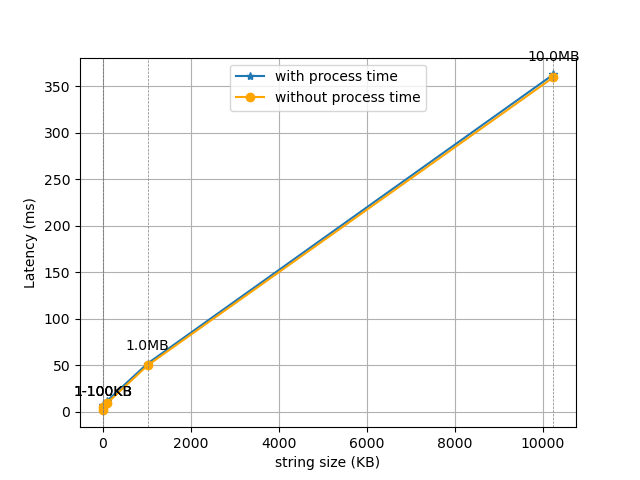
\includegraphics[width=\textwidth]{figures/tests/proportional_tests/Rest_Average_string_messages_sending_time_of_100_tests.png}\hfill 
        \caption{} \label{fig: proportional-rest-stringsize-a}
    \end{subfigure}
    \begin{subfigure}[b]{0.49\textwidth}
        \centering
        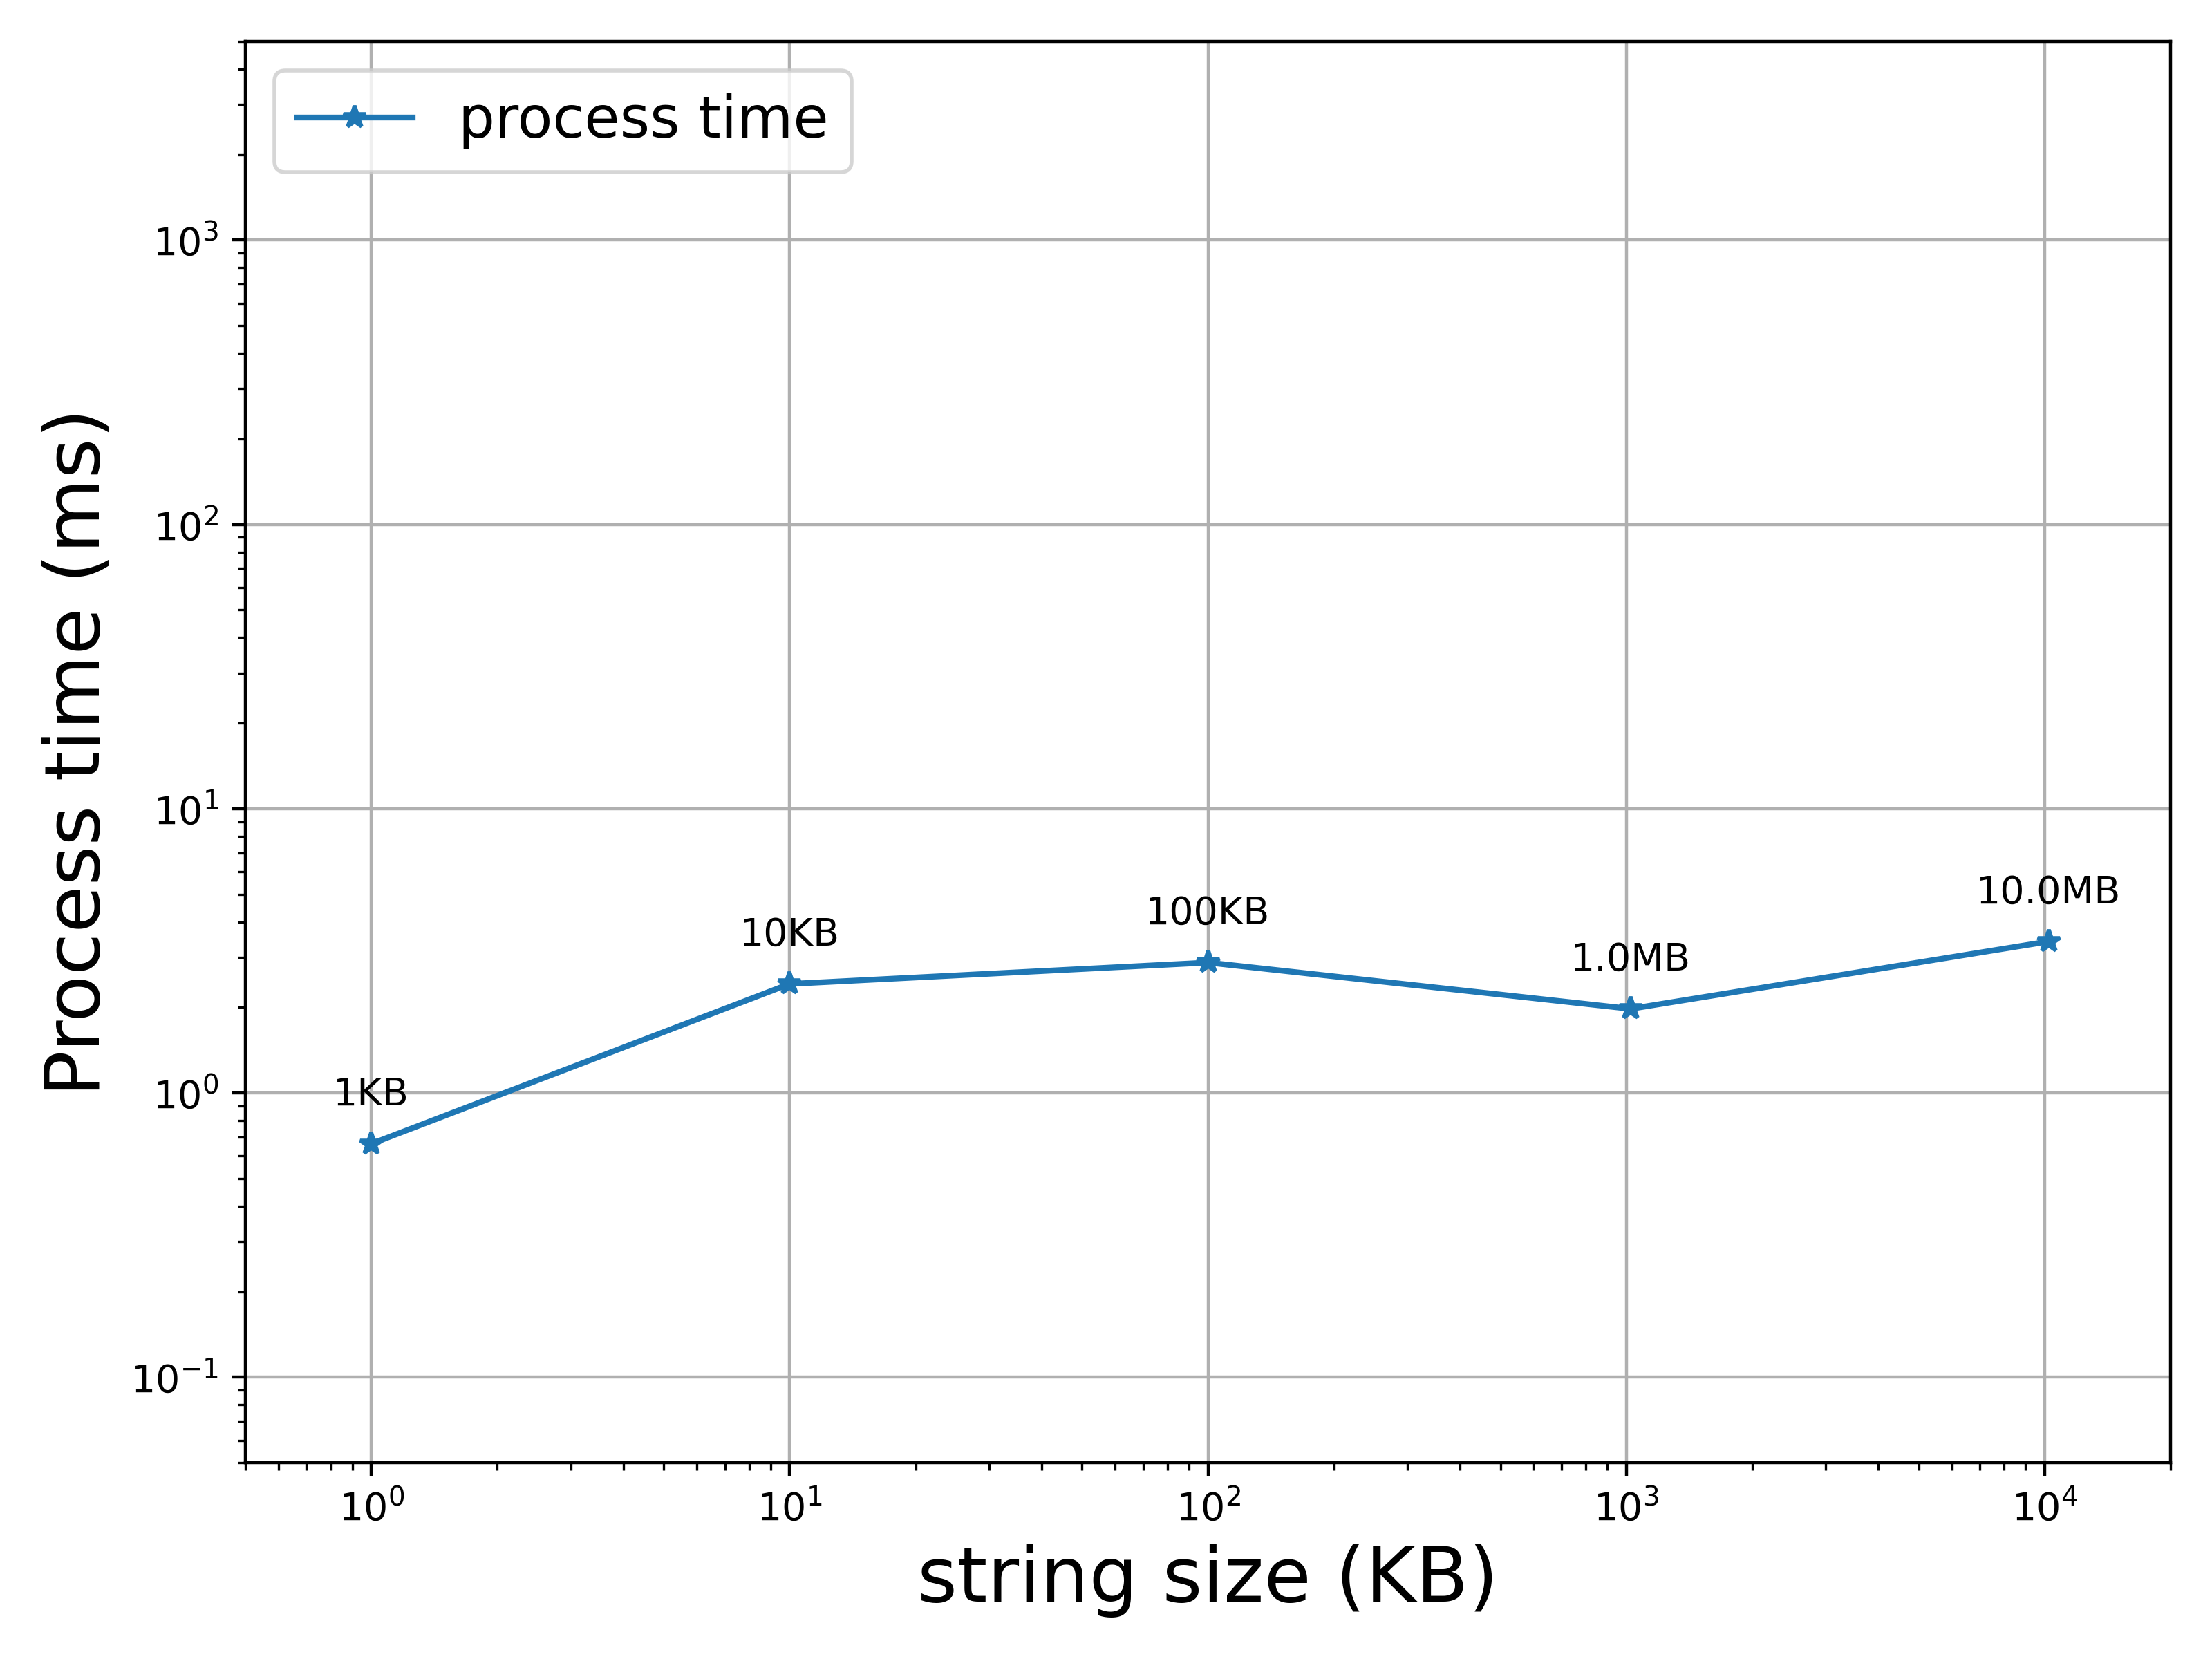
\includegraphics[width=\textwidth]{figures/tests/proportional_tests/Rest_Average_string_messages_receiving_time_of_100_tests.png}\hfill 
        \caption{} \label{fig: proportional-rest-stringsize-b}
    \end{subfigure}
    
    \caption{RESTful API: Average delay of sending and receiving a string message varied from 1KB 
    to 10MB for 100 times between 2 clients. (\subref{fig: proportional-rest-stringsize-c}) 
    Messages clientS sent forward, 
    (\subref{fig: proportional-rest-stringsize-d}) response messages from clientR, 
    (\subref{fig: proportional-rest-stringsize-a}) process time of messages sent forward 
    and (\subref{fig: proportional-rest-stringsize-b}) process time of messages respond. 
    \label{fig: proportional-rest-stringsize}}
\end{figure}





\subsection{Test results of message prioritization in a WebSocket server with various 
performance testing} \label{chap: Result-priority}
In an agent communication system, the server that serves as a \gls{ca} should not only 
focus on speed, robustness, reliability, and application size, but also have additional 
functionalities beyond pure message transport. The design pattern of \gls{ca} should 
include a communication interface 
capable of processing various messages with different data types such as string 
and jsonified images, 
handling a large number of agent connections, and prioritizing incoming messages. 
In the following sections, we will test and discuss the server's performance in 
handling message prioritization. In both tests, we gradually increase the number 
of clients with only one client that sends a critical message, causing the data processing 
of other messages with lower priorities to wait. Except for the client numbers and 
message type, all other conditions remain constant. 

\subsubsection{Measurgin method}
In order to verify the prioritization mechanism of the server, a delay of 1s should be 
added to the non-prioritized message processing. In the test, two kinds of messages are 
sent concurrently to the server: the normal and the critical messages. If multiple 
messages with different priority levels enter the server simultaneously, the critical 
messages should be processed first. The add-up of delay also reflects real-world scenarios. 
Suppose a critical message representing an emergent stop or a task with higher priority 
in production comes in. In that case, every other process in the server should wait until 
the critical message is sent. 

\subsubsection{String message priority test}
The first string priority test is performed for ten clients. The following 
fig.\ref{fig: priority-10clients-a} and \ref{fig: priority-10clients-b} show the 
mean \gls{owd} that a non-prioritized and prioritized message is being sent forward and 
back separately for 100 times.
Fig.\ref{fig: priority-10clients-a} shows the mean \gls{owd} for client1 to client10 in both 
directions, which ranges from 0.63ms to 1.09ms. These results meet the suggested near real-time 
requirement for the production process\cite{li_5g_2018}, with a latency from <1 ms to 10 ms 
for the use of collaborative robots in a factory. 
On the other hand, fig.\ref{fig: priority-10clients-b} 
illustrates the timing differences between normal messages as a group and critical messages 
as a control group. In this test, all clients except client10 delivered normal messages. 
The server paused other processes for 1s and handled the critical message immediately 
whenever a critical message from client10 arrived. The mean \gls{owd} for client10 was less 
than 1ms, while clients such as client1 through client5 and client9 experienced 
significantly higher \gls{owd}, sometimes reaching several hundred milliseconds. This 
verified the assumption of message prioritization. It is worth mentioning that the 
asyncio package used in the WebSocket server design is concurrent. Therefore, each 
client is executed one after another, rather than in parallel processing. As a result, 
some messages may never be paused if the clients' execution process is not synchronized 
and coordinated explicitly.

\begin{sidewaysfigure}[htb]
    \centering
    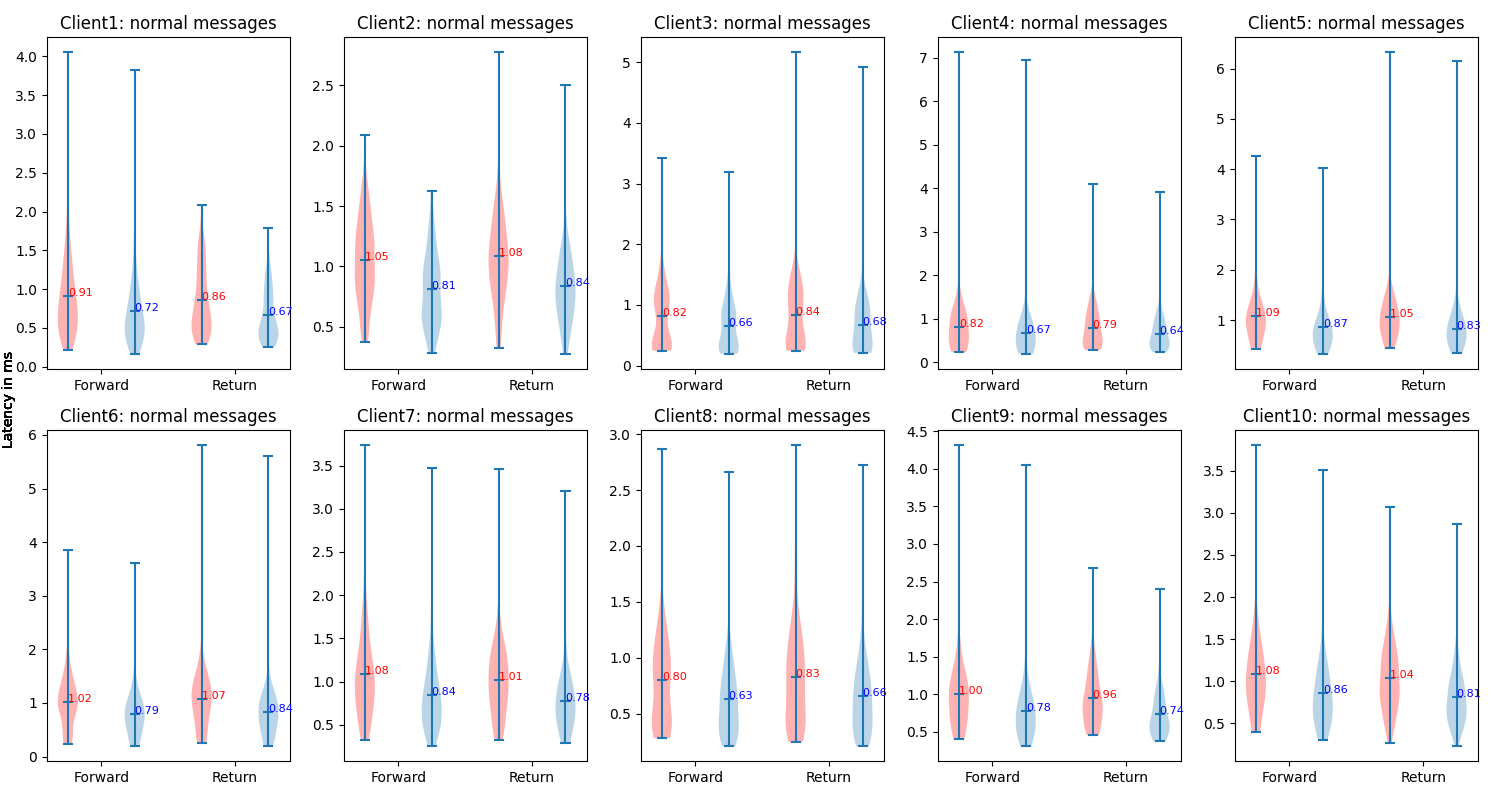
\includegraphics[width=\textheight]{figures/tests/priority_tests/violin_10clients_string_non_priority.png}\hfill 
    \caption{Tests for timing properites of forward and return non-prioritized string messages between 10 clients 
    and clientR for 100 times. The blue violin represents the average data transmission time and the red violin 
    respresent mean \gls{owd}.} \label{fig: priority-10clients-a}
\end{sidewaysfigure}
\begin{sidewaysfigure}[htb]
    \centering
    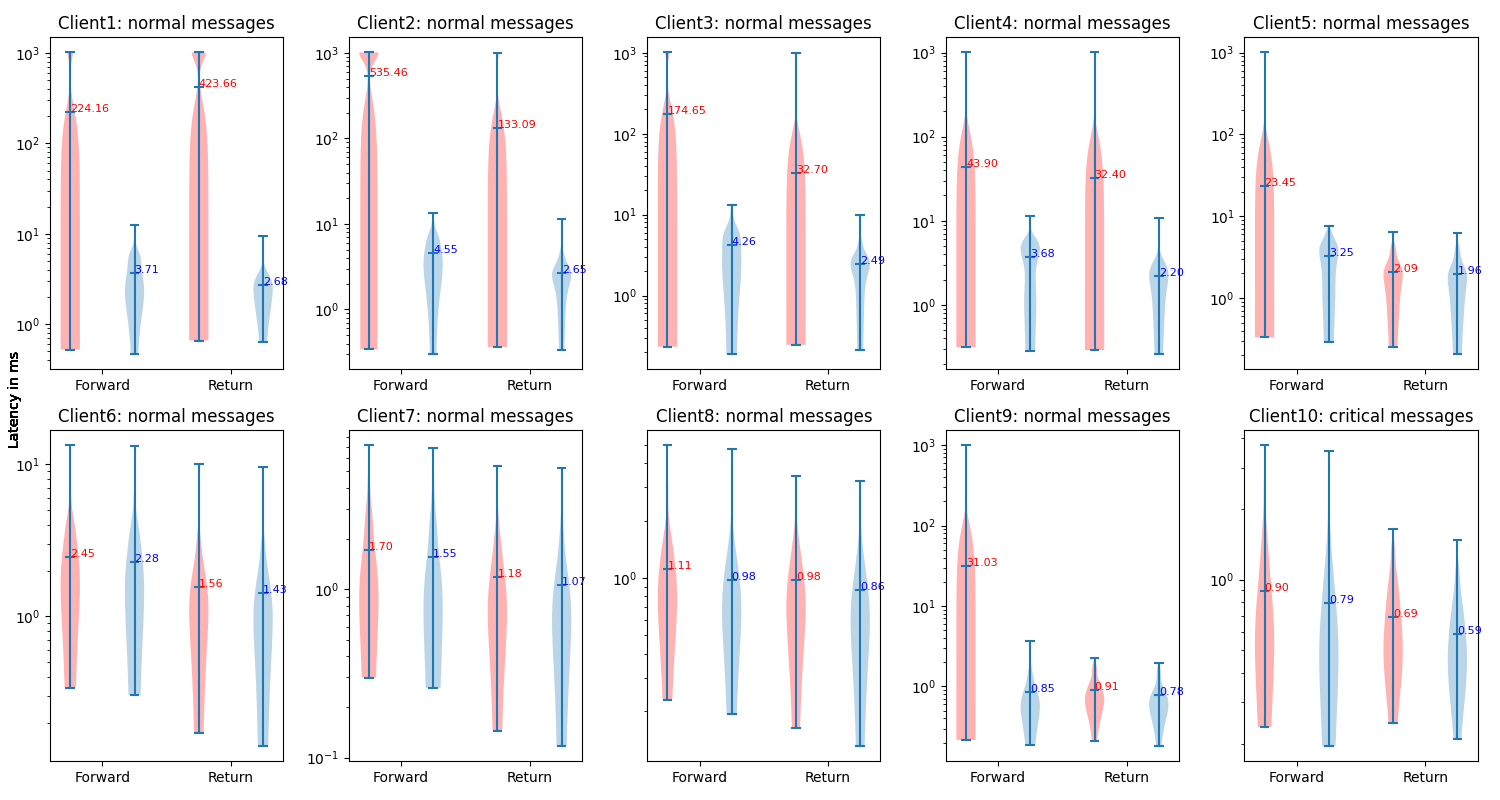
\includegraphics[width=\textheight]{figures/tests/priority_tests/log_violin_10clients_string_priority.png}\hfill 
    \caption{Tests for mean \gls{owd} of forward and return prioritized string messages between 10 clients 
    and clientR for 100 times. The blue violin represents the average data transmission time and the red violin 
    respresent mean \gls{owd}.} \label{fig: priority-10clients-b}
\end{sidewaysfigure}





As part of our testing process, priority tests are performed for ten clients across 
various scales, with the number of clients varying from 2 to 10 to 50. The test results 
of two clients can be found in \ref{chap: append-string-priority} fig.\ref{fig: priority-2clients-string}, 
and those for fifty clients in fig.\ref{fig: priority-50clients-string-a} to 
\ref{fig: priority-50clients-string-e}.  The results of the string message priority 
test with two clients clearly show that client 1 sent messages with lower priority, 
resulting in significantly higher delays than client 2 in both directions. In the test 
with fifty clients, the results were similar to those of the ten-client test. Only the 
last client sent a critical message, while the other 49 sent normal messages. As a 
result, some clients were affected by the mechanism, causing significant delays, while 
client 50 always had the smallest round-trip time.

\subsubsection{JSON message priority test}
The same tests are also done for image message transport. Slightly different from string 
messages, the prioritization jsonified image file (image size: 33.4KB) will be performed 
after deserialization. In the image priority test, client1 to client10 will send an image 
to clientR and receive a string message as a response. In actual production, a confirm 
string message will be sent back if the clientR successfully receives the image message. 
Therefore, this test better reflects the time difference between different message types 
in the actual production process since the actual string length will be much smaller than 
the image length. As shown in fig.\ref{fig: priority-10clients-c}, it proves that the data 
transmission time or the server process time of an image message 
will be higher than that of a string message.


\begin{sidewaysfigure}[htb]
    \centering
    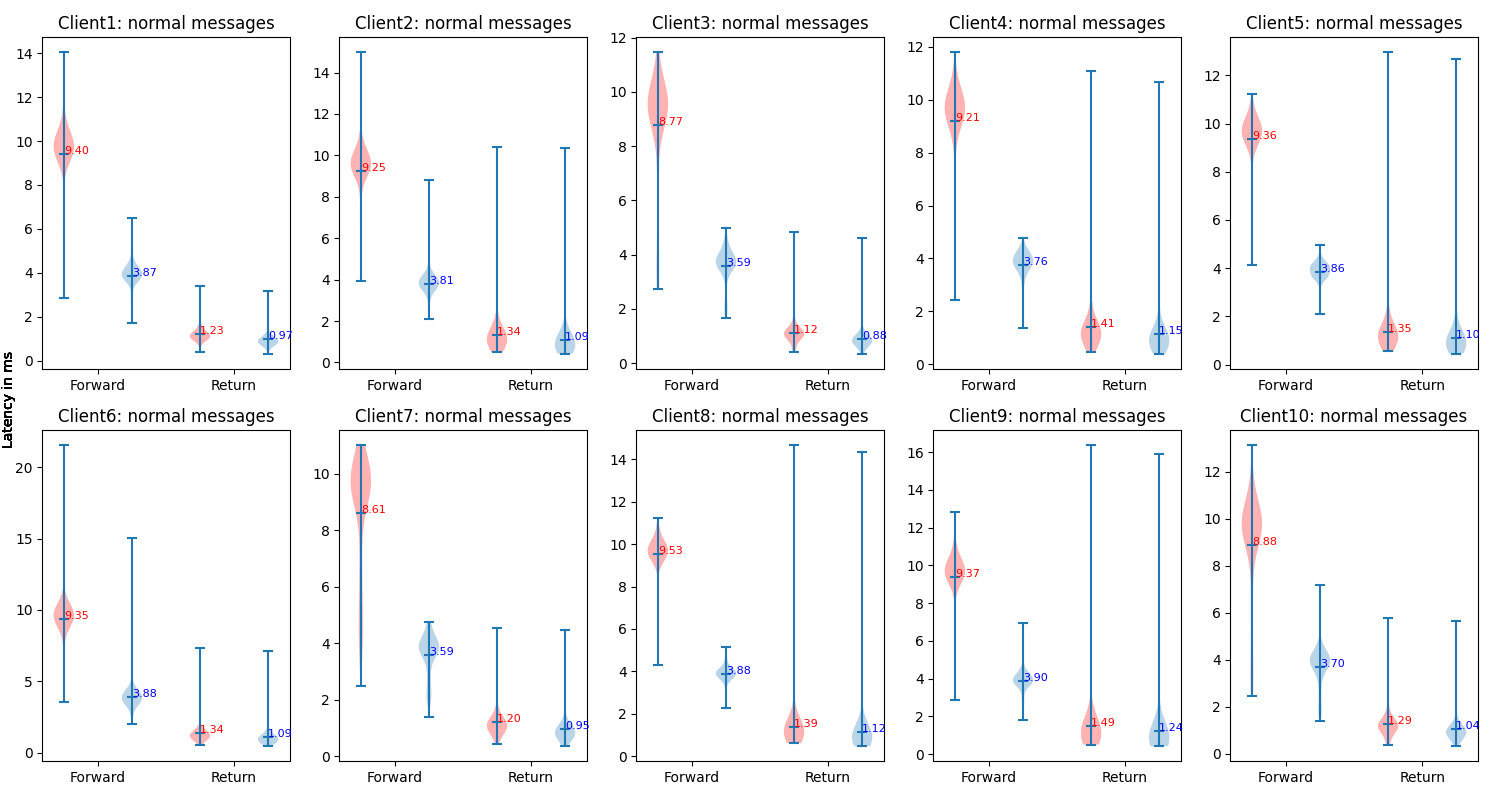
\includegraphics[width=\textheight]{figures/tests/priority_tests/violin_10clients_image_non_priority.png}\hfill 
    \caption{Tests for timing properites of non-prioritized forward jsonified image messages and return string messages between 10 clients 
    and clientR for 100 times. The blue violin represents the average data transmission time and the red violin 
    respresent mean \gls{owd}.} \label{fig: priority-10clients-c}
\end{sidewaysfigure}


Another test (fig.\ref{fig: priority-10clients-d}) should be similar to the string message priority test In the upcoming test (fig.\ref{fig: priority-10clients-d}), 2, 10, and 50 clients will send images and receive string messages as a response from clientR. All clients, except client10, will send normal image messages while client10 will send a critical one to the clientR. The prioritization mechanism will be triggered for all image messages and a part of the response string messages. Notably, the prioritized string messages' latency in this test is similar to the previous test results (fig.\ref{fig: priority-10clients-b}). 

This can be attributed to the fact that larger file sizes require longer transport and 
processing times. As the image message length increases, more data bytes need to be 
processed simultaneously, resulting in more message queuing and prioritization in the 
server. A similar conclusion can be drawn from the tests conducted for 2 and 50 clients 
in fig.\ref{fig: priority-2clients-image} to fig.\ref{fig: priority-50clients-image-e} 
in \ref{chap: append-image-priority}., 
with 2, 10 and 50 clients sending images and receiving string messages as a response 
from clientR. All client1 to client9 send a normal image message, and meanwhile client10 
sends a critical one to the clientR. In the test, all image messages and only a part of 
the response string messages being sent trigger the prioritization mechanism. In this, 
the latency for the prioritized string messages is very similar to previous test results.
The reason might be that the larger the file size, the longer the transport 
and processing time will be required. The more significant message length of images 
results in more data bytes that need to be processed simultaneously, which involves 
more message queuing and prioritization in the server. The same conclusion can also be 
made for the tests for 2 and 50 clients in \ref{chap: append-image-priority} 
fig.\ref{fig: priority-2clients-image} to \ref{fig: priority-50clients-image-e}.


\begin{sidewaysfigure}[htb]
    \centering
    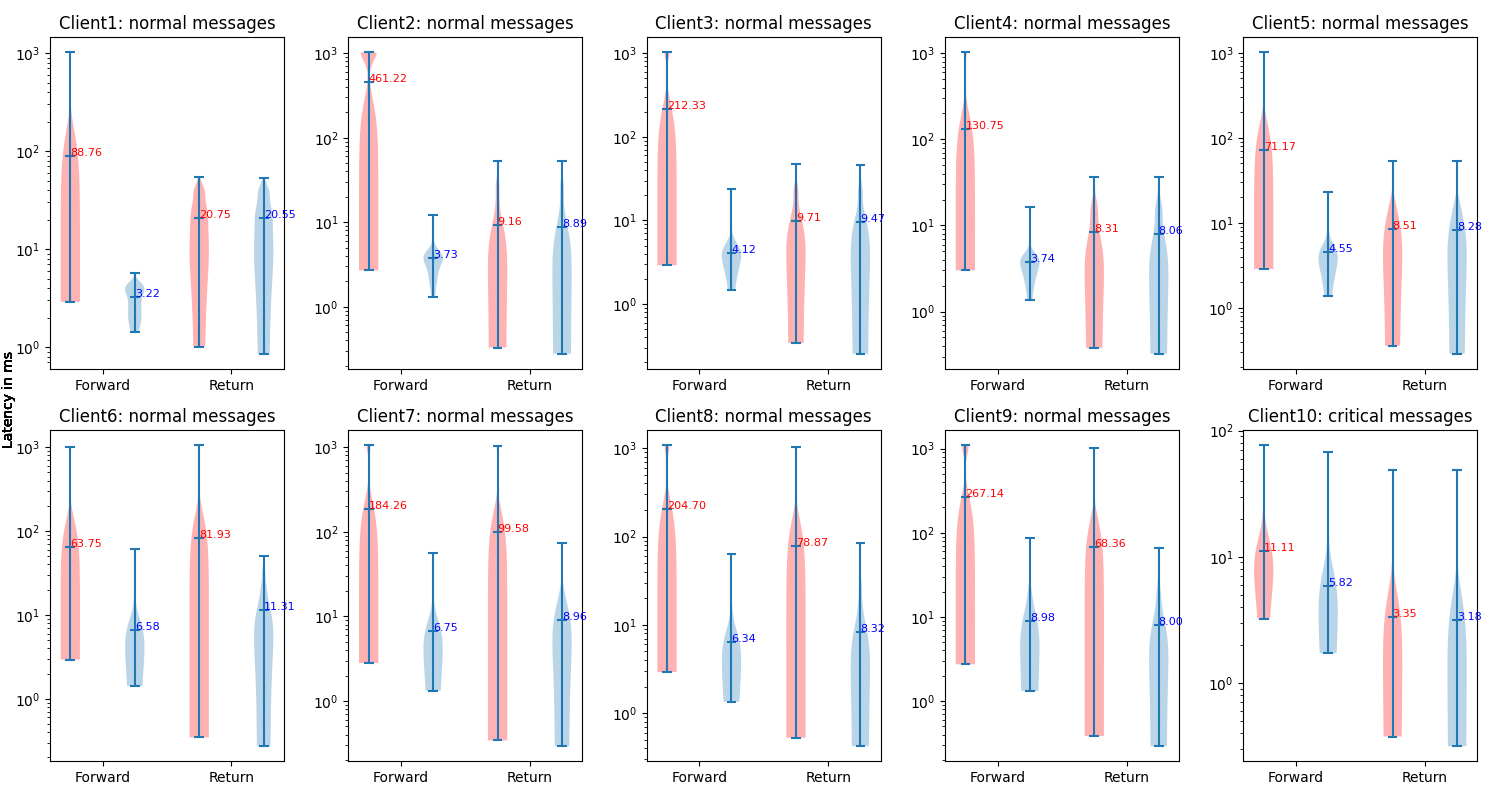
\includegraphics[width=\textheight]{figures/tests/priority_tests/log_violin_10clients_image_priority.png}\hfill 
    \caption{Tests for timing properites of prioritized forward jsonified image messages and return string messages between 10 clients 
    and clientR for 100 times. The blue violin represents the average data transmission time and the red violin 
    respresent mean \gls{owd}.} \label{fig: priority-10clients-d}
\end{sidewaysfigure}


\subsection{Diagrams of \gls{mas} architecture under two use cases and 
test results of BMW use case}\label{chap: Result-Internal-Usecase}

As mentioned earlier in the form of pseudocode in Section \ref{chap: Meth-WS-MAS}, 
the architecture of the \gls{mas} is designed to cater to all use cases. In the code, 
a complete workflow is designed for a standard production process in the real world, 
from agent allocation to sequenced-based agent communication. To gain a better 
understanding of the workflow of both use cases, two diagrams are provided: 
fig.\ref{fig: sequence-diagram} shows a general workflow that can be applied to all
use cases, and fig.\ref{fig: Flowchart-usecase} shows the actual workflow of the 
two use cases.


In the general use case diagram (fig.\ref{fig: sequence-diagram}), the 
design for the \gls{mas} should be identical for all use cases except for 
the availability check and primitive execution parts (production processes) in the loop. 
The detailed program execution sequence is already described in 
section \ref{chap: Meth-WS-MAS}. Something worth noting here is that the sequence 
of the production processes in the loop should be relevant to use cases, namely the 
customer requirements. That means the sequence for task execution in the test should 
be more complex. Rather than a simple round trip between three agents, sometimes the 
Transport agent can receive orders from the Storage agent and send orders to the Storage 
agent again to save time from the slow restocking of supermarket cell. However, 
the workflow in fig.\ref{fig: Flowchart-usecase} may be the best route in actual 
production based on its simplicity of agent communication design.  

\begin{figure}[htb]
    \centering
    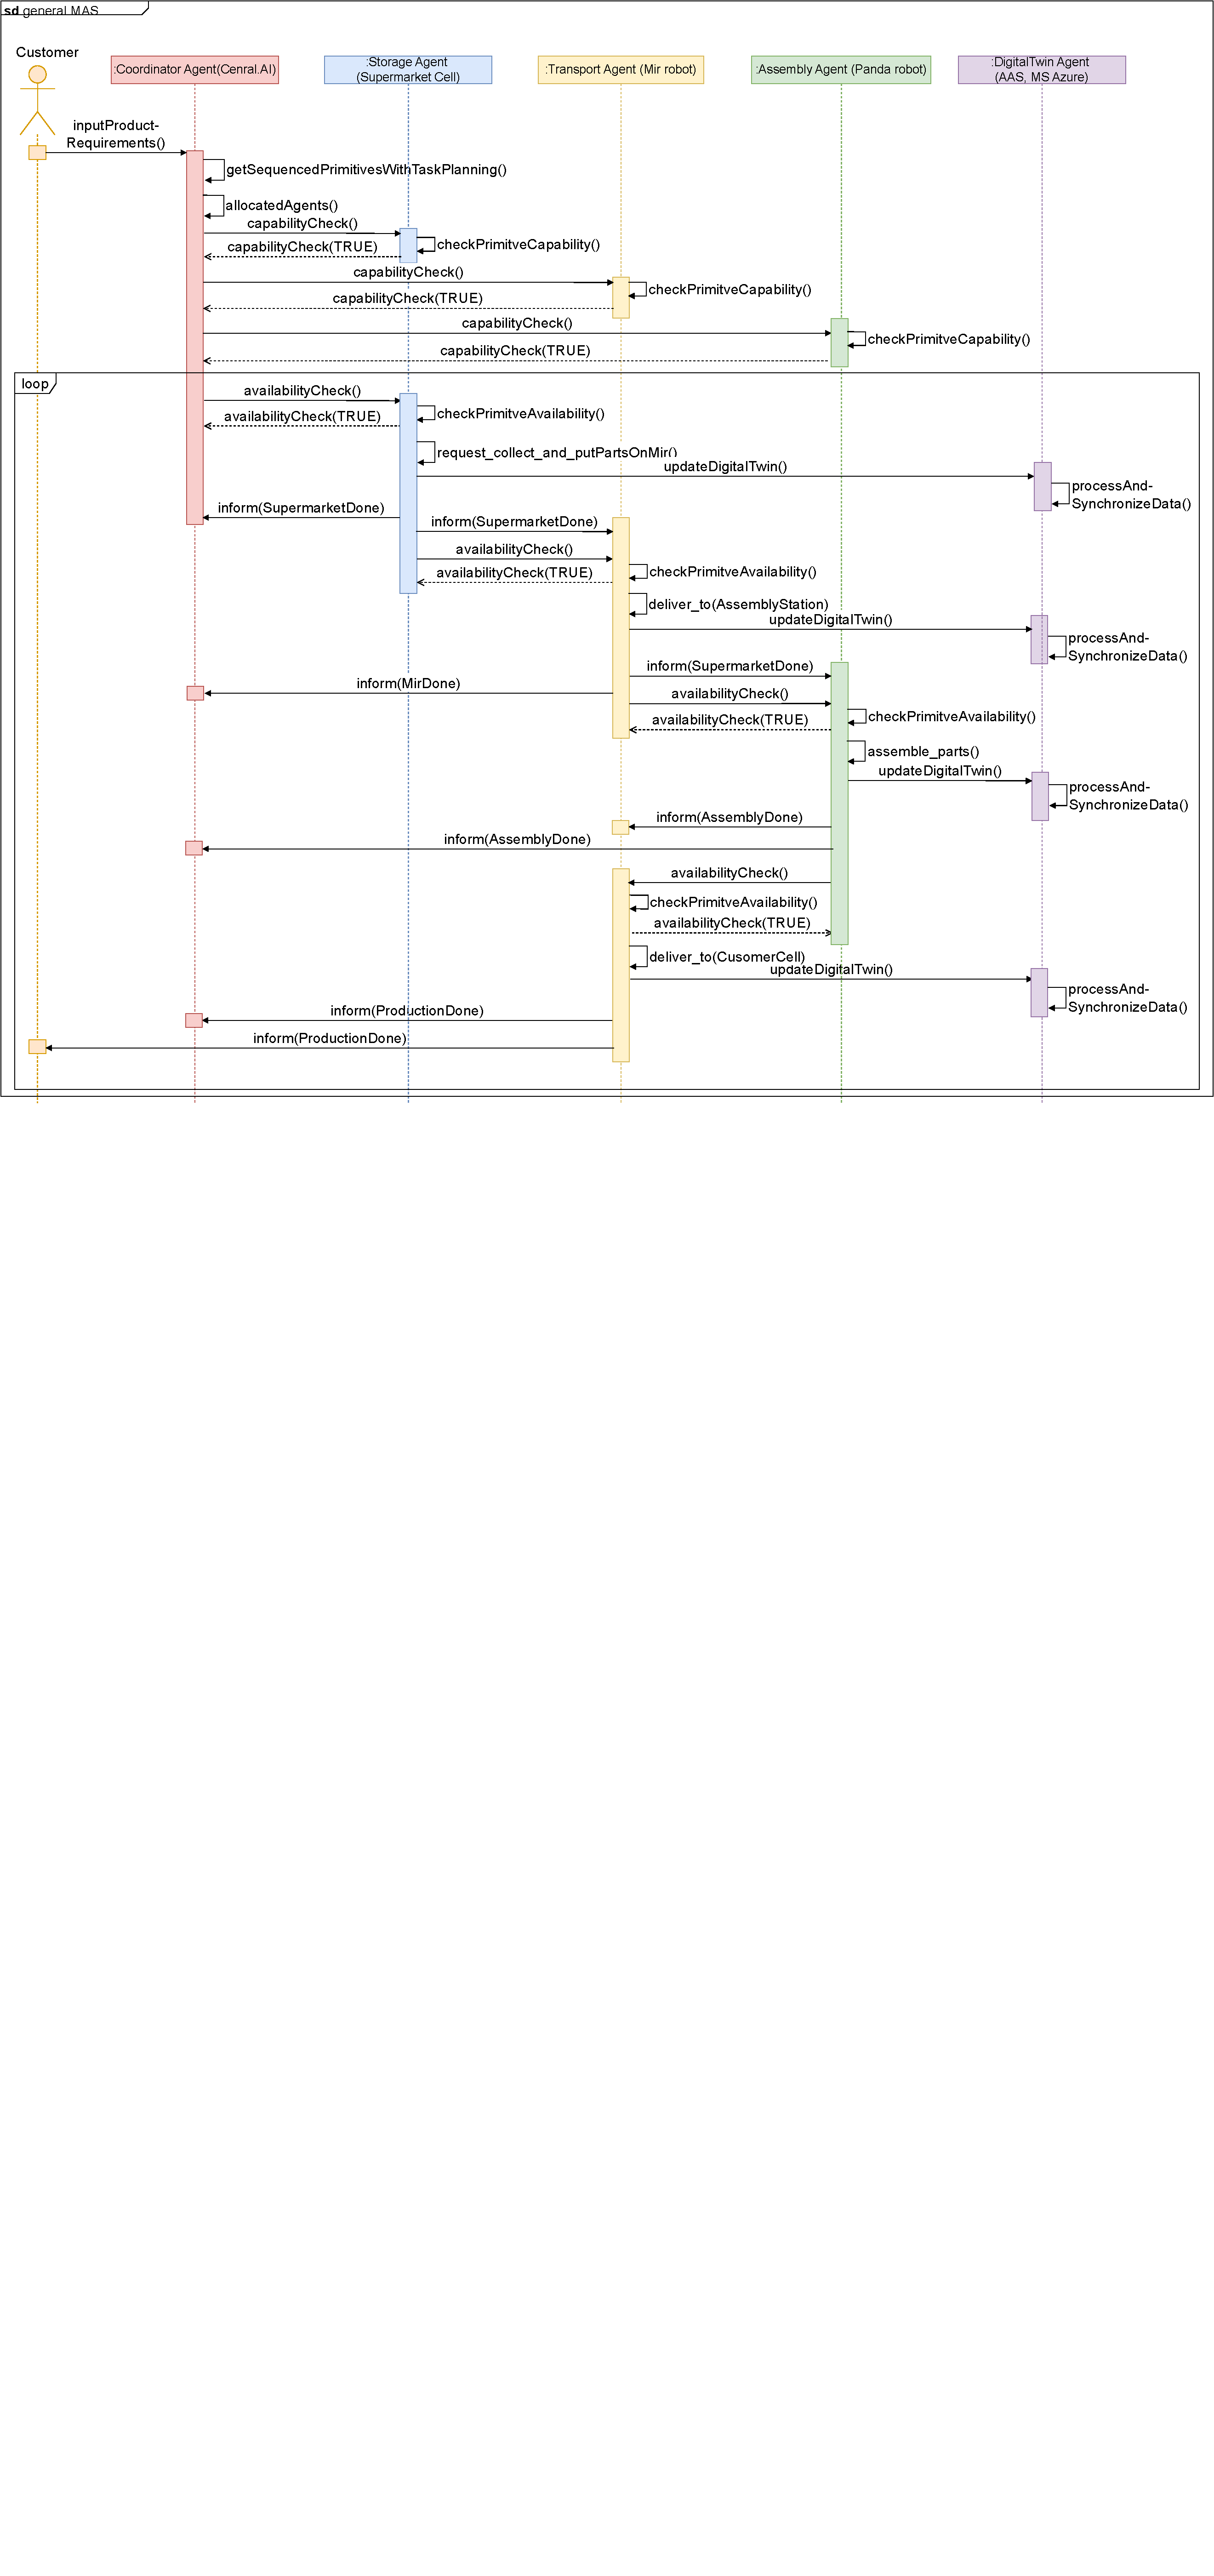
\includegraphics[width=\textwidth]{figures/tests/usecase/SequenceUsecases.pdf}\hfill 
    \caption{sequenced diagram for general use case of the \gls{mas} architecture.} 
    \label{fig: sequence-diagram}
\end{figure}


\begin{figure}[htb]
    \centering
    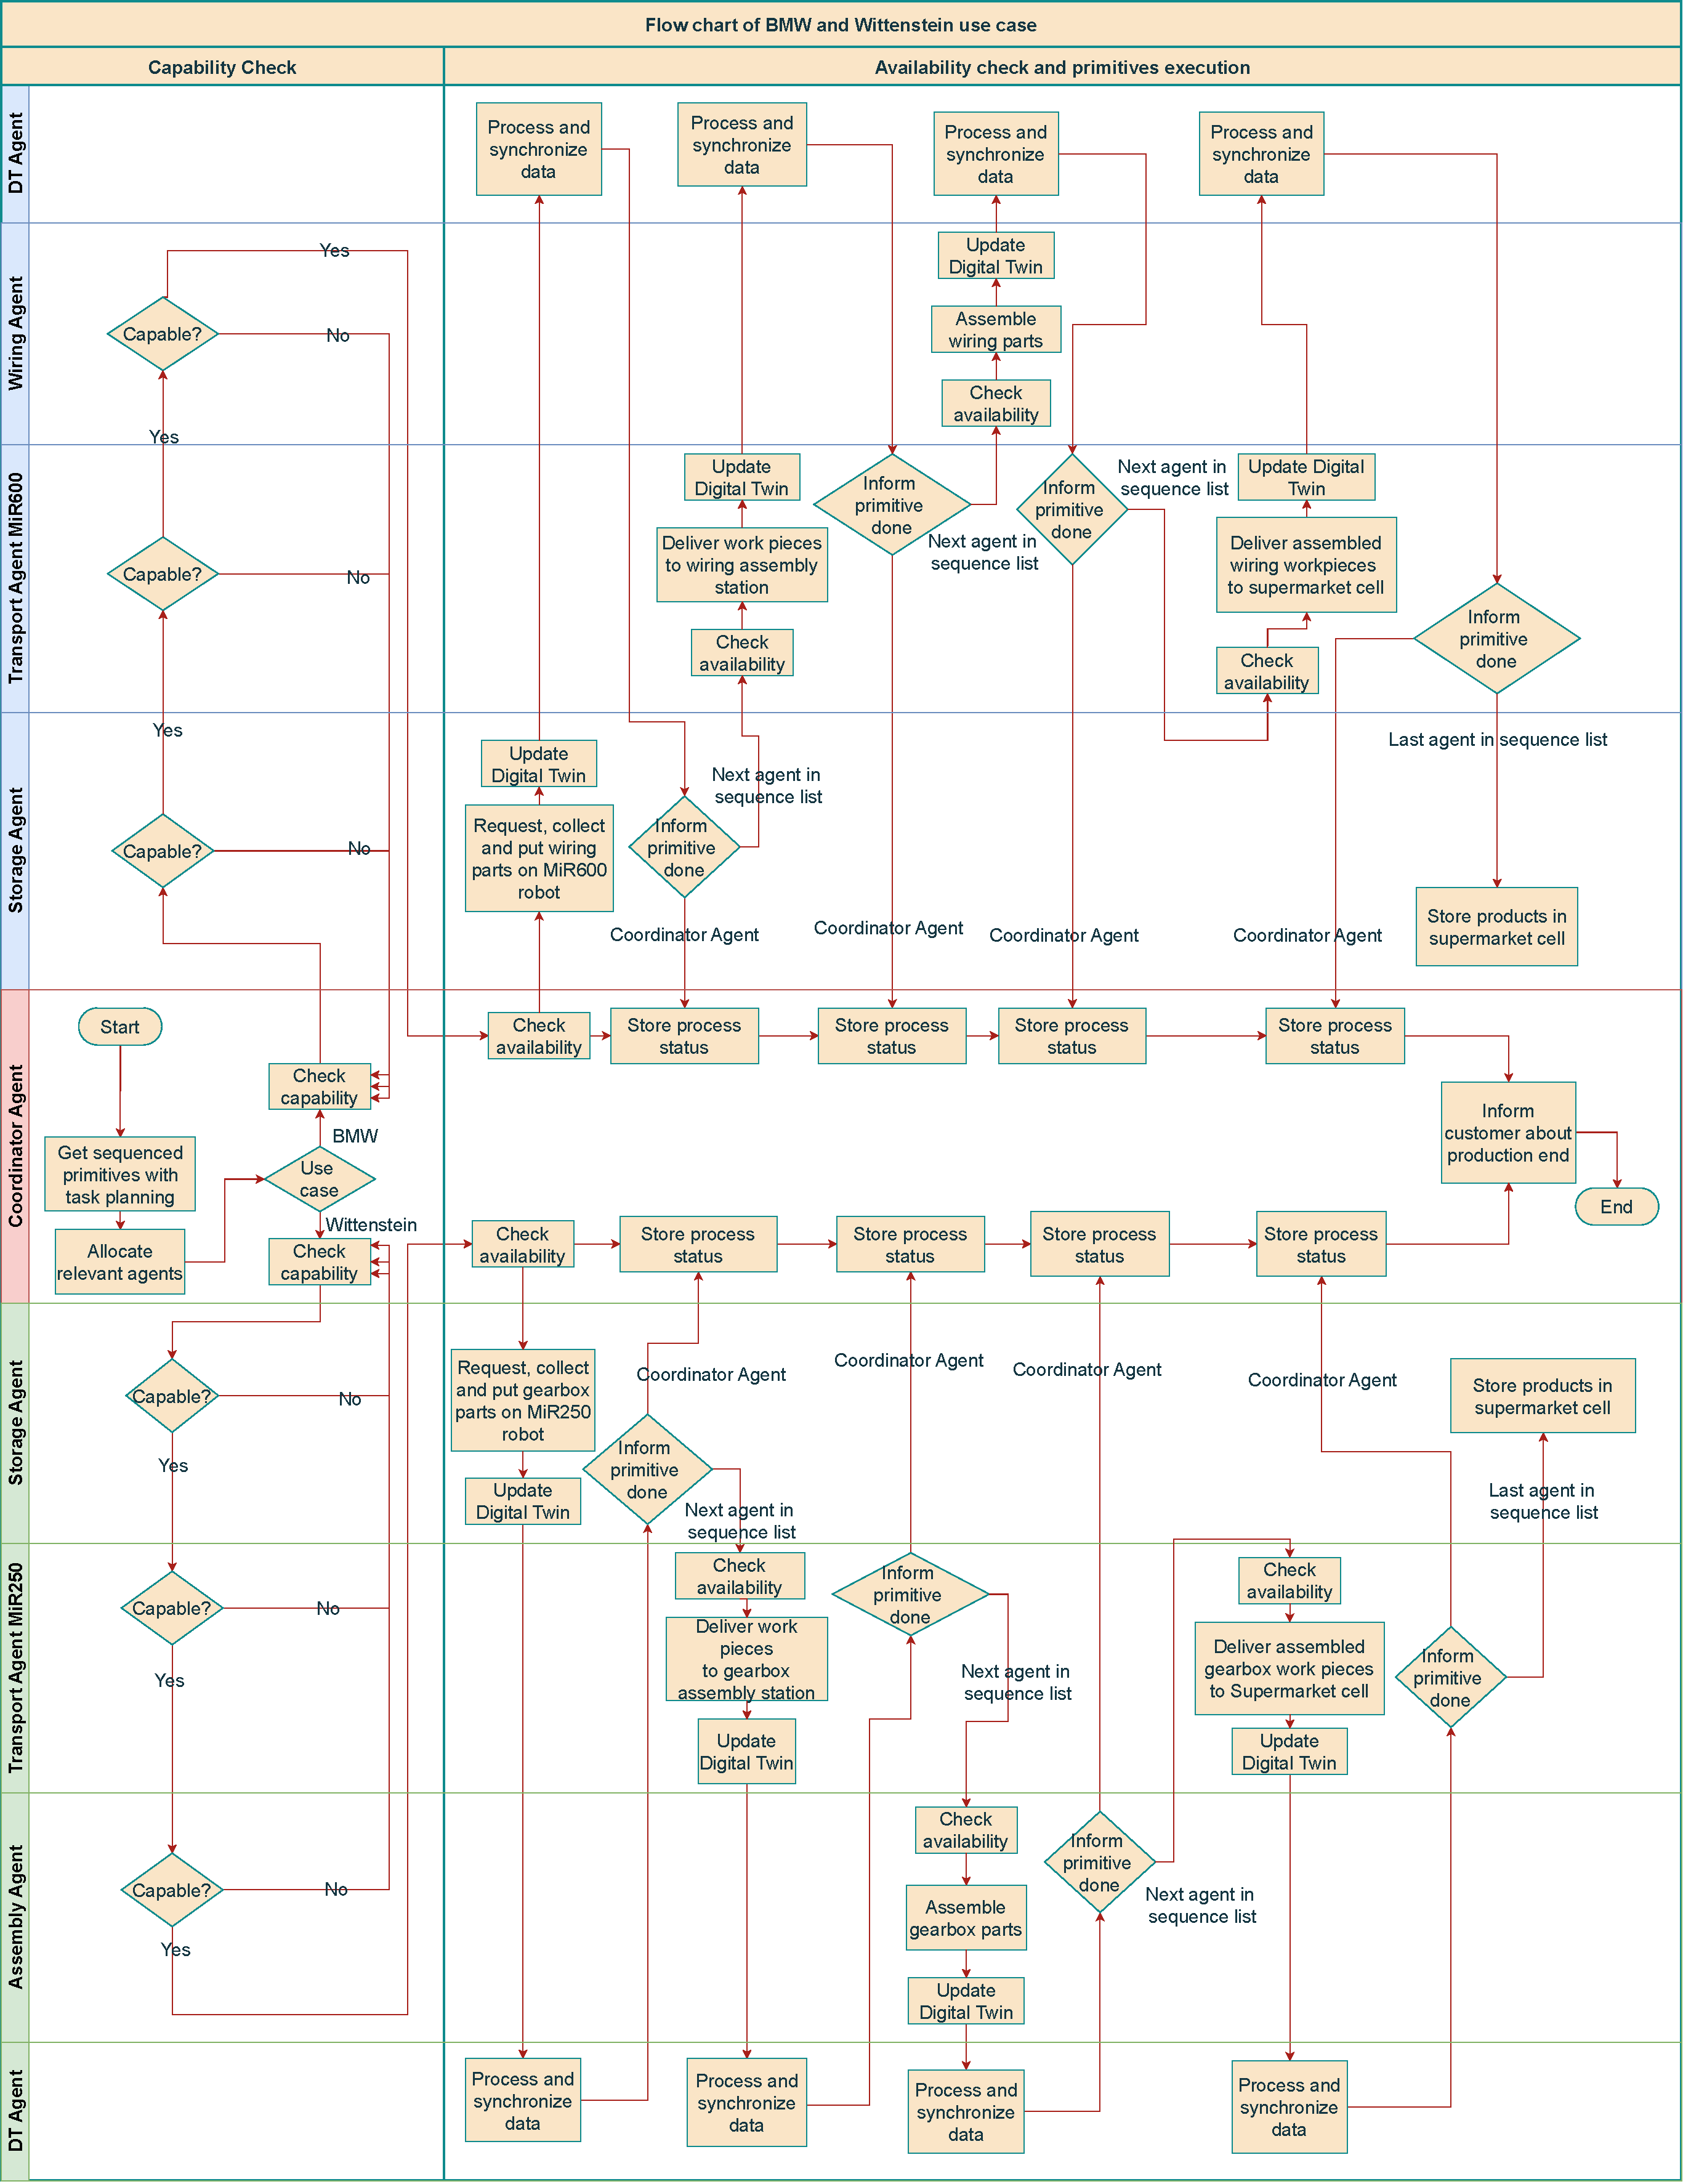
\includegraphics[width=\textwidth]{figures/tests/usecase/Usecase_flow.pdf}\hfill 
    \caption{Flowchart of BMW and Wittenstein use case of the \gls{mas} architecture. 
    Blue containers: BMW use case, allocated agents are Storge agent, 
    Transport agent MiR600, Wiring agent and \gls{dta} respectively. 
    Green Containers: Wittenstein use case, allocated agents are Storage agent, 
    Transport agent MiR250, Assembly agent and \gls{dta} respectively. 
    Red container: \gls{cda} for both usecases.} 
    \label{fig: Flowchart-usecase}
\end{figure}
The primitives, agents and execution sequence for both BMW and Wittenstein use cases 
are predefined. However, only the timing behaviors of the BMW use case are tested due 
to similarity. The average \gls{owd} and WebSocket data transmission time of the BMW 
use case are presented in table \ref{tab: mean-usecase-time}, with a excerpt of the whole 
data table for BMW use case presented in table \ref{tab: TestsCDAMiR600}. The test was conducted 
100 times, but the number of messages exchanged among agents varied greatly. Therefore, 
the test results and average values can only be used as a reference to understand the 
data transmission process in actual production. In order to provide a more detailed data 
distribution of each message, the violin plot in fig.\ref{fig: violin-CDA-T600} is 
presented along with other test results with other agents (see fig.\ref{fig: violin-CDA-ST} to \ref{fig: violin-T600-WI}). 
Based on these results, it can be concluded that the message transport in the system meets 
the real-time requirements, with the largest message size of 636 Bytes taking a maximum of 
10ms and the smallest taking about 0.2ms.


% Please add the following required packages to your document preamble:
% \usepackage{graphicx}
% \usepackage{lscape}

\begin{table}[b]
    \tiny
    \centering
    \caption{An excerpt of communication messages from \gls{cda} to Transport Agent MiR600, the full table can be found in \ref{firstfootnote}.}
    \label{tab: TestsCDAMiR600}
    \begin{tabular}{m{0.1\textwidth} m{0.1\textwidth} m{0.05\textwidth} m{0.05\textwidth} m{0.35\textwidth} m{0.07\textwidth} m{0.05\textwidth}}
    \hline
    \textbf{Sender}            & \textbf{Recipient}              & \textbf{Message number} & \textbf{Message length (Bytes)} & \textbf{Message content}                                                                                                                                                                                                                                                                                                                                                                                                                                                                                                                                                                                                                      & \textbf{Transmission time (ms)} & \textbf{OWD (ms)} \\ \hline
    Coordinator Agent & TransportAgent MiR600 & 1  & 34  & "TransportAgent\_MiR600:normal:Are you ready?"                                                                                                                                                                                                                                                                                                                                                                                                                                                                                                                                                                                                                                           & 1.099 & 0.923 \\ 
    & & & & & &\\
    Coordinator Agent & TransportAgent MiR600 & 2  & 53  & "TransportAgent\_MiR600:normal:Are you capable:move\_MIR"                                                                                                                                                                                                                                                                                                                                                                                                                                                                                                                                                                                                                                & 0.982 & 0.805 \\ 
    & & & & & &\\
    Coordinator Agent & TransportAgent MiR600 & 3  & 62  & "TransportAgent\_MiR600:normal:Are you capable:pick\_up\_shelf\_MIR"                                                                                                                                                                                                                                                                                                                                                                                                                                                                                                                                                                                                                     & 0.920 & 0.730 \\ 
    & & & & & &\\
    Coordinator Agent & TransportAgent MiR600 & 4  & 67  & "TransportAgent\_MiR600:normal:Are you capable:get\_position\_transport"                                                                                                                                                                                                                                                                                                                                                                                                                                                                                                                                                                                                                 & 1.011 & 0.816 \\ 
    & & & & & &\\
    Coordinator Agent & TransportAgent MiR600 & 5  & 53  & "TransportAgent\_MiR600:normal:Are you capable:move\_MIR"                                                                                                                                                                                                                                                                                                                                                                                                                                                                                                                                                                                                                                & 1.046 & 0.840 \\ 
    & & & & & &\\
    Coordinator Agent & TransportAgent MiR600 & 6  & 60  & "TransportAgent\_MiR600:normal:Are you capable:place\_shelf\_MIR"                                                                                                                                                                                                                                                                                                                                                                                                                                                                                                                                                                                                                        & 1.058 & 0.845 \\ 
    & & & & & &\\
    Coordinator Agent & TransportAgent MiR600 & 7  & 53  & "TransportAgent\_MiR600:normal:Are you capable:move\_MIR"                                                                                                                                                                                                                                                                                                                                                                                                                                                                                                                                                                                                                                & 0.987 & 0.778 \\ 
    & & & & & &\\
    Coordinator Agent & TransportAgent MiR600 & 8  & 60  & "TransportAgent\_MiR600:normal:Are you capable:place\_shelf\_MIR"                                                                                                                                                                                                                                                                                                                                                                                                                                                                                                                                                                                                                        & 0.981 & 0.767 \\ 
    & & & & & &\\
    Coordinator Agent & TransportAgent MiR600 & 9  & 53  & "TransportAgent\_MiR600:normal:Are you capable:move\_MIR"                                                                                                                                                                                                                                                                                                                                                                                                                                                                                                                                                                                                                                & 1.023 & 0.829 \\ 
    & & & & & &\\
    Coordinator Agent & TransportAgent MiR600 & 10 & 60  & "TransportAgent\_MiR600:normal:Are you capable:place\_shelf\_MIR"                                                                                                                                                                                                                                                                                                                                                                                                                                                                                                                                                                                                                        & 1.008 & 0.800 \\ 
    & & & & & &\\
    Coordinator Agent & TransportAgent MiR600 & 11 & 52  & "TransportAgent\_MiR600:normal:Finish capability check"                                                                                                                                                                                                                                                                                                                                                                                                                                                                                                                                                                                                                                  & 0.947 & 0.752 \\ 
    & & & & & &\\
    Coordinator Agent & TransportAgent MiR600 & 12 & 324 & "TransportAgent\_MiR600:normal:Sequence:{[}{[}1, 1, 0{]}, {[}1, 1, 0{]}, {[}1, 2, 0{]}, {[}1, 2, 0{]}, {[}1, 2, 0{]}, {[}1, 2, 1{]}, {[}1, 2, 2{]}, {[}1, 2, 3{]}, {[}1, 2, 4{]}, {[}1, 2, 5{]}, {[}1, 2, 6{]}, {[}1, 2, 7{]}, {[}1, 2, 8{]}, {[}1, 3, 0{]}, {[}1, 3, 0{]}, {[}1, 3, 0{]}, {[}2, 1, 0{]}, {[}2, 1, 0{]}, {[}2, 1, 0{]}, {[}2, 1, 1{]}, {[}2, 2, 0{]}, {[}2, 2, 1{]}, {[}2, 2, 2{]}, {[}2, 2, 3{]}, {[}2, 3, 0{]}, {[}2, 3, 1{]}{]}"                                                                                                                                                                                                                                      & 1.082 & 0.849 \\ 
    & & & & & &\\
    Coordinator Agent & TransportAgent MiR600 & 13 & 547 & "TransportAgent\_MiR600:normal:All\_Primitives:{[}'Get\_cable\_routing', 'Get\_shoplist\_BMW', 'move\_initial\_panda', 'move\_MIR', 'pick\_up\_shelf\_MIR', 'read\_shoplist', 'get\_position\_shop', 'get\_item\_shoprobot', 'move\_panda', 'close\_gripper\_data', 'get\_position\_transport', 'move\_panda', 'open\_gripper', 'move\_initial\_panda', 'move\_MIR', 'place\_shelf\_MIR', 'move\_MIR', 'place\_shelf\_MIR', 'move\_initial\_wiring\_panda', 'pick\_up\_components', 'identify\_cable\_color', 'calculate\_position', 'execute\_wiring', 'place\_shelf\_component', 'move\_MIR', 'place\_shelf\_MIR'{]}"                                                                  & 1.023 & 0.780 \\ 
    & & & & & &\\
    Coordinator Agent & TransportAgent MiR600 & 14 & 528 & "TransportAgent\_MiR600:normal:Sequenced\_agents:{[}'StorageAgent', 'StorageAgent', 'StorageAgent', 'TransportAgent\_MiR600', 'TransportAgent\_MiR600', 'StorageAgent', 'StorageAgent', 'StorageAgent', 'StorageAgent', 'StorageAgent', 'TransportAgent\_MiR600', 'StorageAgent', 'StorageAgent', 'StorageAgent', 'TransportAgent\_MiR600', 'TransportAgent\_MiR600', 'TransportAgent\_MiR600', 'TransportAgent\_MiR600', 'WiringAgent', 'WiringAgent', 'WiringAgent', 'WiringAgent', 'WiringAgent', 'WiringAgent', 'TransportAgent\_MiR600', 'TransportAgent\_MiR600'{]}" & 1.083 & 0.820 \\ 
    & & & & & &\\
    Coordinator Agent & TransportAgent MiR600 & 15 & 29  & "TransportAgent\_MiR600:normal:"                                                                                                                                                                                                                                                                                                                                                                                                                                                                                                                                                                                                                                                         & 1.207 & 0.956 \\ 
    & & & & & &\\
    Coordinator Agent & TransportAgent MiR600 & 16 & 29  & "TransportAgent\_MiR600:normal:"                                                                                                                                                                                                                                                                                                                                                                                                                                                                                                                                                                                                                                                         & 1.106 & 0.874 \\ 
    & & & & & &\\
    Coordinator Agent & TransportAgent MiR600 & 17 & 29  & "TransportAgent\_MiR600:normal:"                                                                                                                                                                                                                                                                                                                                                                                                                                                                                                                                                                                                                                                         & 1.172 & 0.930 \\ 
    & & & & & &\\
    Coordinator Agent & TransportAgent MiR600 & 18 & 29  & "TransportAgent\_MiR600:normal:"                                                                                                                                                                                                                                                                                                                                                                                                                                                                                                                                                                                                                                                         & 1.474 & 1.196 \\ \hline
    \end{tabular}%

\end{table}


\begin{table}[b]
    \small
    \centering
    \caption{Average delays between agents with different string message length and 
    different amount of messages.}
    \label{tab: mean-usecase-time}
    \begin{tabular}{|m{0.13\textwidth}|m{0.17\textwidth}|m{0.17\textwidth}|m{0.17\textwidth}|m{0.17\textwidth}|}
    \hline
    \multicolumn{5}{|c|}{\textbf{Average delays between agents (\gls{owd}/Transmission time)}}                                                            \\ \hline
    \textbf{}                         & \textbf{Coordinator Agent}             & \textbf{Storage Agent}        & \textbf{Transport Agent MiR600}    & \textbf{Wiring Agent}\\ \hline
    \textbf{Coordinator Agent}      & None                  & 1.029355ms /0.820172ms & 1.067170ms /0.849335ms  & 1.032151ms /0.817049ms \\ \hline
    \textbf{Storage Agent}          & 0.998253ms /0.794590ms & None                  & 1.427890ms /1.158142ms  & None                  \\ \hline
    \textbf{Transport Agent MiR600} & 1.055389ms /0.840291ms & 1.422970ms /1.150696ms & None                   & 1.668750ms /1.344250ms \\ \hline
    \textbf{Wiring Agent}           & 0.988012ms /0.783014ms & None                  & 1.654000ms /1.361000ms  & None                  \\ \hline
    \end{tabular}
\end{table}


\begin{figure}[htb]
    \centering
    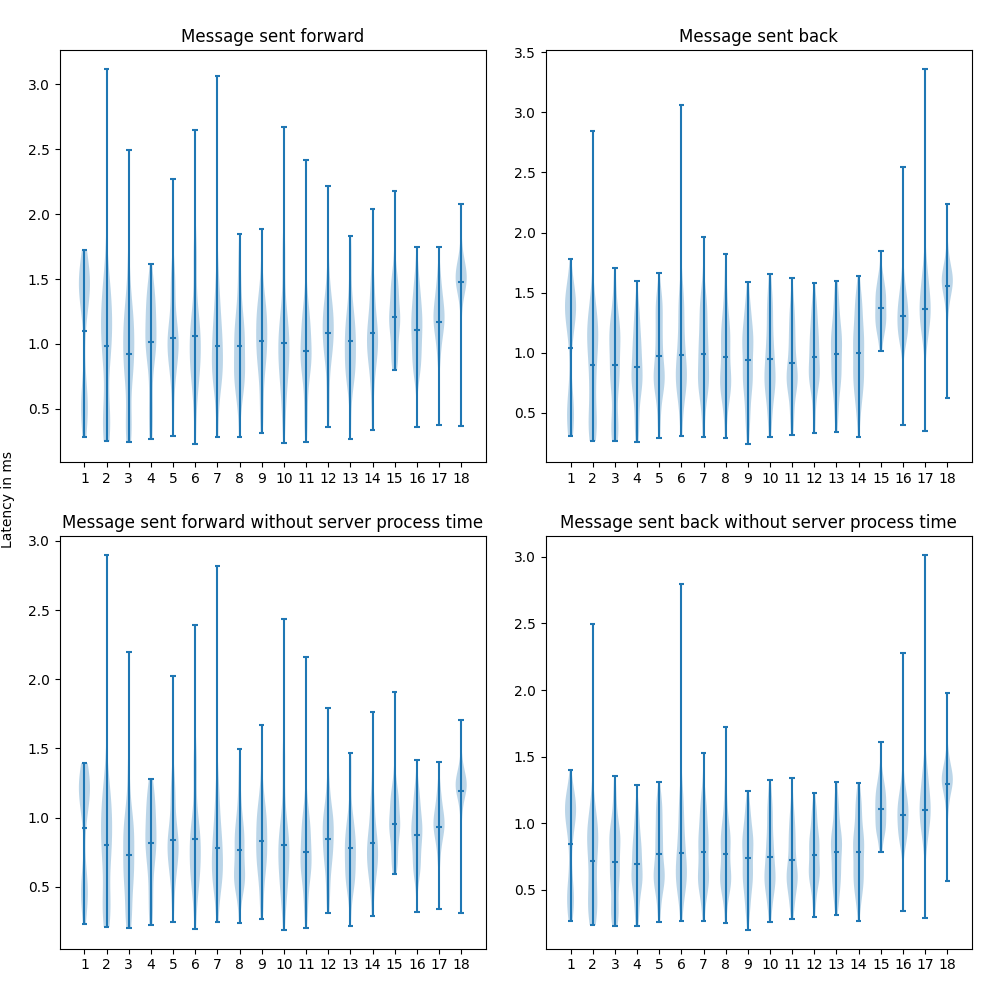
\includegraphics[width=\textwidth]{figures/tests/usecase/violin_CoordinatorAgent_to_TransportAgent_MiR600.png}\hfill 
    \caption{Test to measure \gls{owd} and transmission time between \gls{cda} and 
    TransportAgent\_MiR600 for 100 times. The number in x-axis respresents the 
    corresonding messages \protect\ref{firstfootnote}.}
    \label{fig: violin-CDA-T600}
\end{figure}

%addtional for footnote in caption
\footnotetext[1]{\label{firstfootnote}https://github.com/XuezhouHou/Websocket\_MAS/blob/master/Table\_with\_all\_values/table4UCBMW.xlsx}



\section{Global \gls{dt}}\label{chap: Result-External}
Second part of the study focuses on the delay measurement of the global \gls{dta} system, tests for the 
upload and download are done separately, with different packet sizes as tuning 
parameters. The pseudocode of the \gls{dta} with a related \gls{rcp} is provided 
in section \ref{chap: RCPDTAPseudo}. To test the performance of \gls{dta} program, 
we first differentiate the delays of a packet with different 
sizes delivered from \gls{rcp} to \gls{dta} through a \gls{tcp} socket. Then we investigate 
delays for the same packet, between \gls{dta} and Azure \gls{dt} through APIs based on 
\gls{http}. Finally, the the same upload and download processes between \gls{dta} and 
Azure \gls{dt} with different patch size are also tested. Different from \gls{mas}, 
the server process time in \gls{dta} is not measured. Hence, in the tests below, 
\gls{owd} is identical to data transmission time. 

\subsection{Pseudocode of \gls{rcp} and \gls{dta} workflow in C++ and C\#}\label{chap: RCPDTAPseudo}

As previously mentioned in this chapter, it is important to completely separate the 
\gls{dta} from the \gls{mas}. Algorithms \ref{alg:RCPPseudoCode} and 
\ref{alg:DTAgentPseudoCode} list the workflows of \gls{rcp} and \gls{dta} separately. 
In the \gls{rcp} workflow, the robot arm is controlled through predefined functions 
that can record the current states. Each new state recorded must be immediately sent 
to the \gls{dta} via the established \gls{tcp} socket. 
On the \gls{dta} side, it must be started before the \gls{rcp} and listen to the 
socket to receive the data stream once connected. Whenever a new connection to a 
\gls{ra} is established, the \gls{dta} will create a new thread to receive, process, 
upload and download data concurrently. 
However, an issue with using \gls{tcp} is that packets do not arrive individually 
but are stuck together. To solve this, delimiters are utilized for sticky packet separation.

%pseudo code for RCP
\begin{breakablealgorithm}
    \caption{Pseudocode of \gls{rcp} workflow}
    \label{alg:RCPPseudoCode}
    \begin{algorithmic}
    \State {Import} socket, franka
    \State {Initialize} \gls{dta}\_IP
    \State \textbf{function} {$get\_rstate\_and\_send(clientSocket)$}
        \State \qquad Start robot motion and record robot state
        \State \qquad {$send\_message(robotState, clientSocket)$}
    \State \textbf{function} {$send\_message(msg, clientSocket)$}
        \State \qquad send robot state to \gls{dta} 
    \State \textbf{Main:}
    \State \qquad Instantiate robot
    \State \qquad Initialize start position
    \State \qquad Establish a \gls{tcp} connection with \gls{dta}  
    \State \qquad {$get\_rstate\_and\_send(clientSocket)$}
    \State \textbf{End}
    \end{algorithmic}
\end{breakablealgorithm}


%pseudo code for DTAgent
\begin{breakablealgorithm}
    \caption{Pseudocode of \gls{dta} workflow}
    \label{alg:DTAgentPseudoCode}
    \begin{algorithmic}
    \State {Import} socket, AzureDigitalTwin
    \State {Initialize} \gls{rcp}\_IP(s)
    \State \textbf{function} {$read\_and\_upload\_download\_processData(\gls{rcp}\_IP)$}
        \State \qquad \textbf{do run in parallel}
            \State \qquad \qquad $create\_client\_thread(\gls{rcp}\_IP)$       
    \State \textbf{function} {$create\_client\_thread(\gls{rcp}\_IP)$}
        \State \qquad Establish a \gls{tcp} connection with \gls{ra}
        \State \qquad {$data = read\_data(clientSocket)$}  
        \State \qquad {$process\_data\_upload\_and\_download(data)$}    
    \State \textbf{function} {$read\_data(clientSocket)$}
        \State \qquad receive and store robot state data
        \State \qquad \textbf{return} data
    \State \textbf{function} {$process\_data\_upload\_and\_download(data)$}
        \State \qquad separate sticky packets with delimiter
        \State \qquad upload processed data to Azure \gls{dt} in json patch
        \State \qquad download twin after data update 
    \State \textbf{Main:}
        \State \qquad \textbf{for} \gls{rcp}\_IP in IPs \textbf{do}
        \State \qquad \qquad {$read\_and\_upload\_download\_processData(\gls{rcp}\_IP)$}
        \State \textbf{End}
    \end{algorithmic}
\end{breakablealgorithm}


\subsection{Test results of data transmission 
time in \gls{tcp} sockets between robots and \gls{dta} across 
various packet lengths} \label{chap: Result-RCP-DTA}

To better measure the influence of different packet lengths on transmission time from 
a \gls{rcp} to \gls{dta} utilizing \gls{tcp} sockets, the packet length of JointGripper 
(joint and gripper of the robot arm) position values should be larger than that of the 
Elbow (elbow of the robot arm), they are 151 and 80 Bytes respectively. As depicted in 
fig.\ref{fig: SR-JointGripper-Elbow}, the mean transmission time of JointGripper is 
larger than Elbow, which verifies that larger files take longer to transfer. 
The cumulative delays of both data lengths also show a linear growth relationship in 
the upper graph, which means there are no major fluctuations or irregularities in 
transmission speeds or times for the packets in \gls{tcp} sockets. 


\begin{figure}[htb]
    \centering
    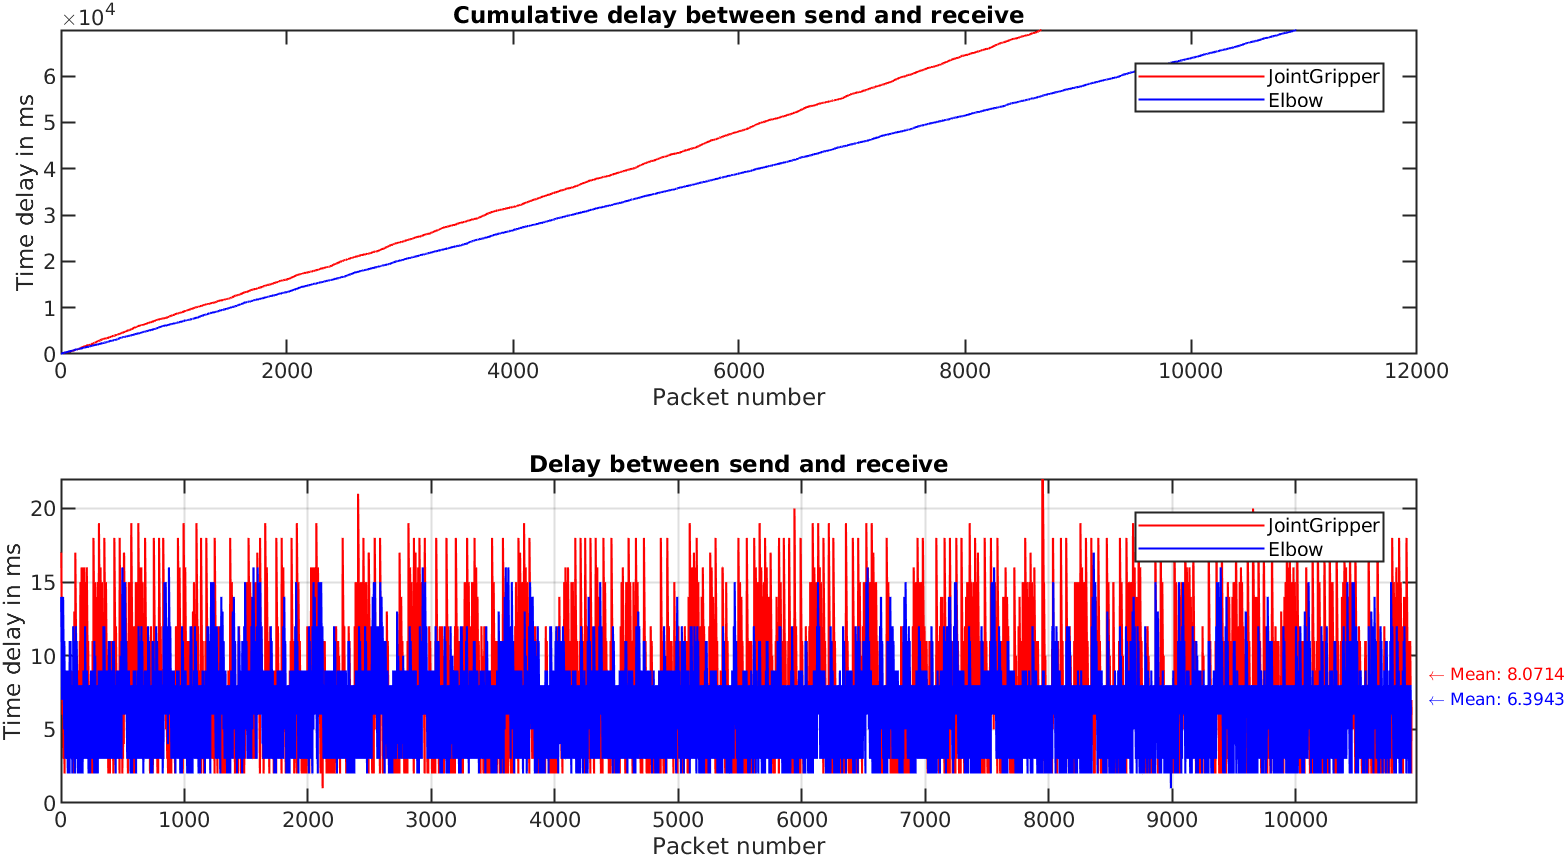
\includegraphics[width=\textwidth]{figures/tests/DT/Delay_SendReceive_JointGripper_Elbow.png}
    \caption{Tests for different packet sizes w.r.t \gls{owd} from \gls{rcp} 
    to \gls{dta}. \label{fig: SR-JointGripper-Elbow}}
\end{figure}

Since each packet only takes a few milliseconds to be transported, the real-time 
requirement for production processes is again fulfilled. 



\subsection{Test results of data transmission time in \gls{tcp} sockets between \gls{dta} 
and \gls{ms} Azure \gls{dt} platform across various packet lengths} \label{chap: Result-DTA-DT}

However, in the program, the most considerable variable of 
the total data transmission time is the \gls{rtt} between local devices and the global digital 
twin. In addition to the \gls{rtt}, the data upload and download time is also measured 
separately, which has an opposite result as those from the research\cite{cainelli_performance_2023}. 
In the paper, the resulting uplink data transmission time is larger than the downlink 
data transmission time. The difference between both tests is that, research team from 
Magdeburg measured delay with logical links from a 5G standalone network and the industrial 
5G devices. In contrast, our test was based on data update times in the cloud. The latency 
between data upload and update reflects the actual \gls{dt} data update patterns, 
which includes additional process time in the cloud. Therefore, we can infer that the 
increased latency of data upload may be caused by the internal Azure \gls{dt} Model 
API for data update (an unclosed issue in \gls{ms} Q\&A\footnote[2]{https://learn.microsoft.com/en-us/answers/questions/1328803/experiencing-slow-load-times-on-azure-digital-twin}).
    

It is worth mentioning that the data upload time from JointGripper and Elbow has little to 
no difference since the upload mechanism of Azure \gls{dt} is limited by sending twin 
values one after one. There is no integrated APIs to update multiple twins simultaneously. 
In order to differentiate the upload speed, the patch size of the to-be-updated twin values 
should vary. The fig.\ref{fig: UD-cycle-JointGripper} again shows the cumulative delays 
with the same conclusion as in fig.\ref{fig: SR-JointGripper-Elbow} and mean \gls{rtt} is 
slightly lower than 100ms, which is still near the real-time requirements with its half 
(compared to the realtime requirements of the end-to-end latency for 5G remote control\cite{li_5g_2018}). 
The packet for 
upload and download will be routed to the cloud, which not only goes through the internal 
5G network but also the internet externally, which results in much higher latency. Compared 
with the test results from \cite{cainelli_performance_2023}, optimizing the internal twin 
update mechanisms can further reduce data \gls{rtt}. 


\begin{figure}[htb]
    \centering
    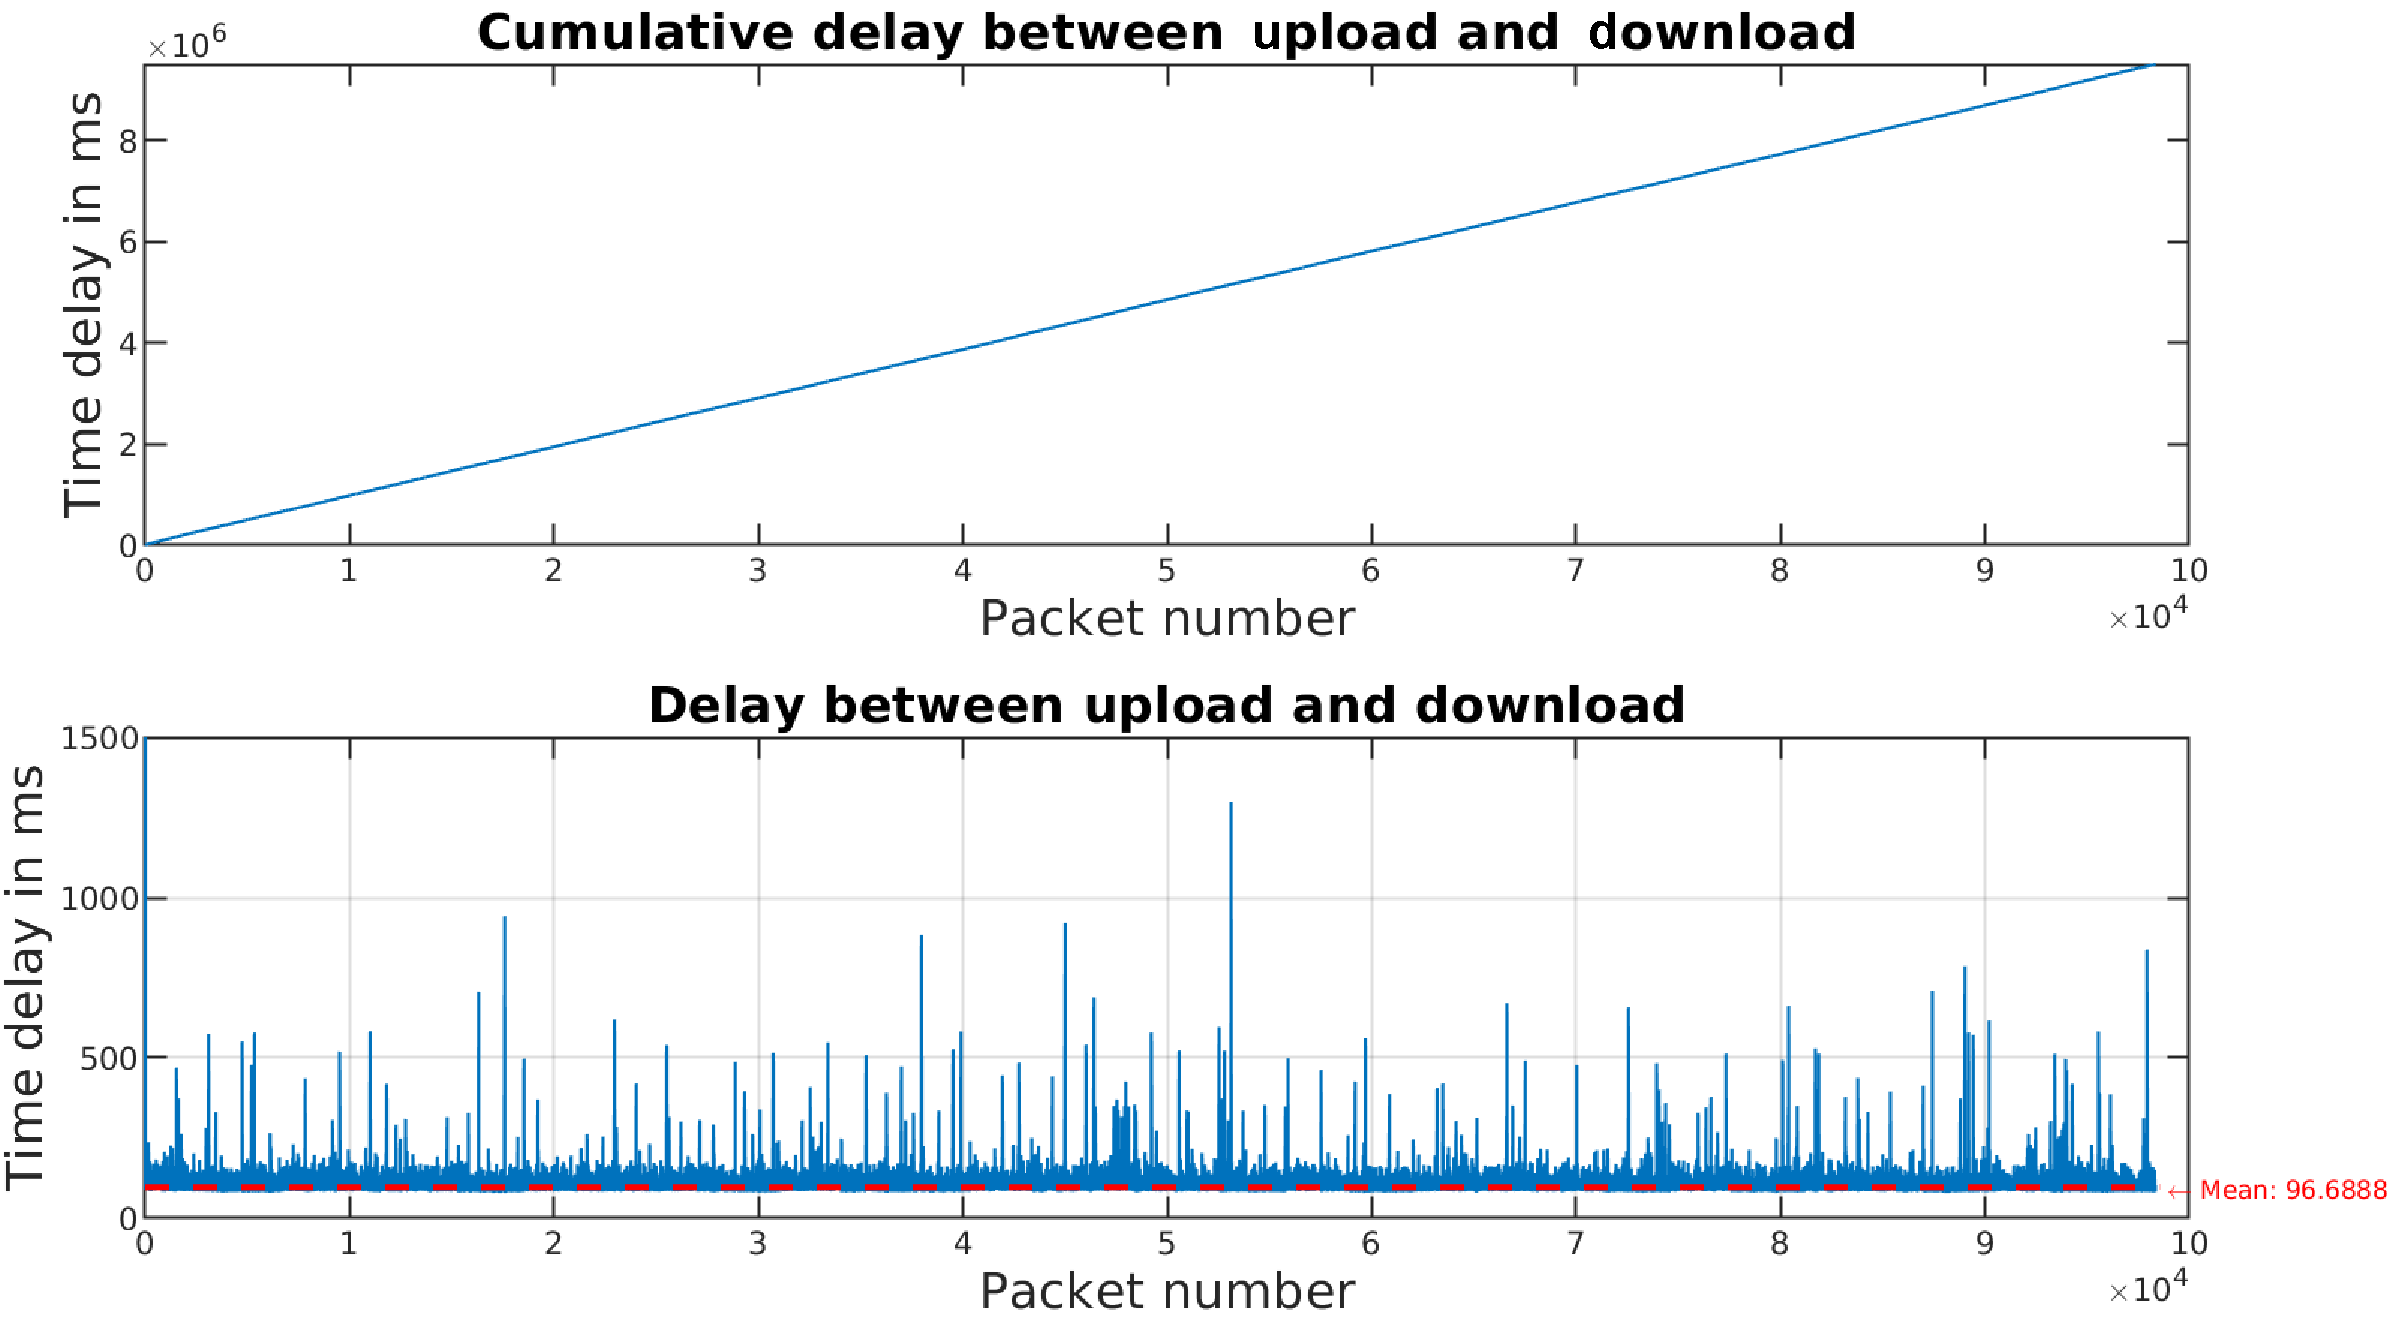
\includegraphics[width=\textwidth]{figures/tests/DT/Delay_UploadDownloadCycleTime_JointGripper.pdf}
    \caption{Tests for \gls{rtt} of data upload and download for JointGripper. \label{fig: UD-cycle-JointGripper}}
\end{figure}

As mentioned, the data upload time is larger than the download time, as depicted in 
fig.\ref{fig: UD-sep-JointGripper}. The average upload time of JointGripper values is under 30ms, 
while the download time results in about 70ms. Under the same conditions, the differences 
between JointGripper and Elbow in both values for are negligible with only 1-2ms difference (see \ref{chap: append-DTagent} fig.\ref{fig: UD-cycle-Elbow} 
and \ref{fig: UD-sep-Elbow}), due to the one after one twin upload mechanism. However, 
the time spent connecting to the \gls{dt} platform needs to be factored in 
as well, which takes about 9400ms for JointGripper and 9600ms for Elbow. Although it 
does not fulfill the real-time requirement, it is still counted for comparison 
to the average download time.




\begin{figure}[htb]
    \centering
    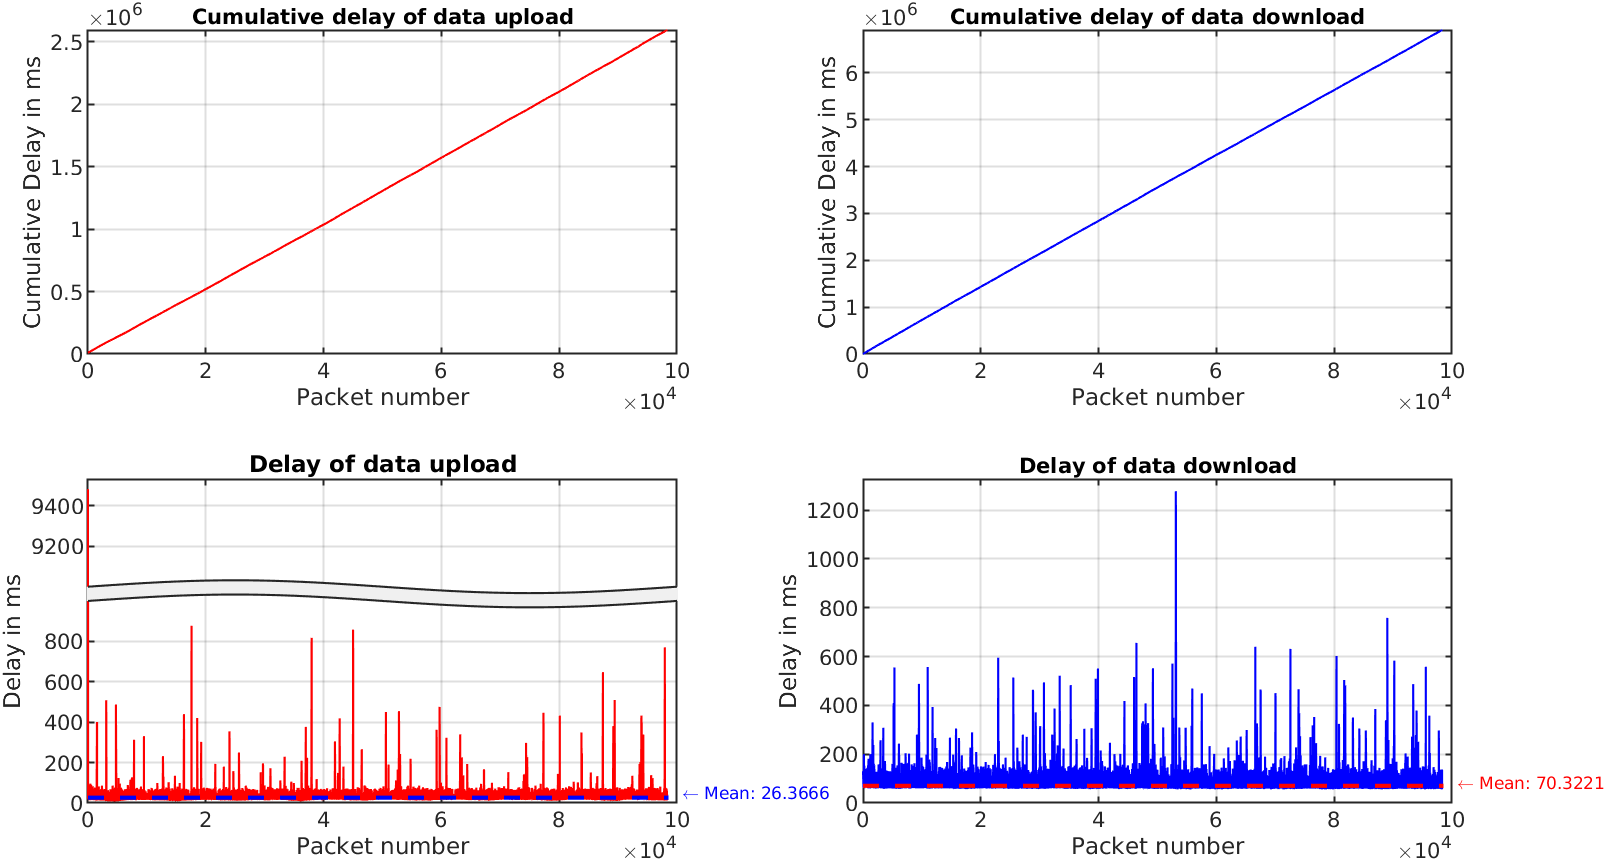
\includegraphics[width=\textwidth]{figures/tests/DT/Delay_UploadDownload_JointGripper.png}
    \caption{Tests for \gls{owd} from \gls{dta} to \gls{dt} update of JointGripper, 
    and \gls{owd} for twin value download. \label{fig: UD-sep-JointGripper}}
\end{figure}


To differentiate the upload speed based on packet size, two patches with 
different sizes are introduced. Ideally, the small data patch with a size of 
49 Bytes should induce a higher transmission speed than the large one with 554 Bytes, 
but the reality is quite different. The test results of all the 
delay measurements for both patch sizes are presented as a violin plot in 
fig.\ref{fig: UD-violin-patchsize}. As expected, the upload time of large 
patches is more than that of small patches, while the result of download time is 
the opposite. This results in nearly identical total \gls{rtt} of both. 
The reasons can be that each test is done at a different time, which results in a 
fluctuation related to the network traffic, cloud service loads, amount of end users 
under the same 5G network, and many more, which influence the data transmission time 
even more than the patch sizes.

\begin{figure}[htb]
    \centering
    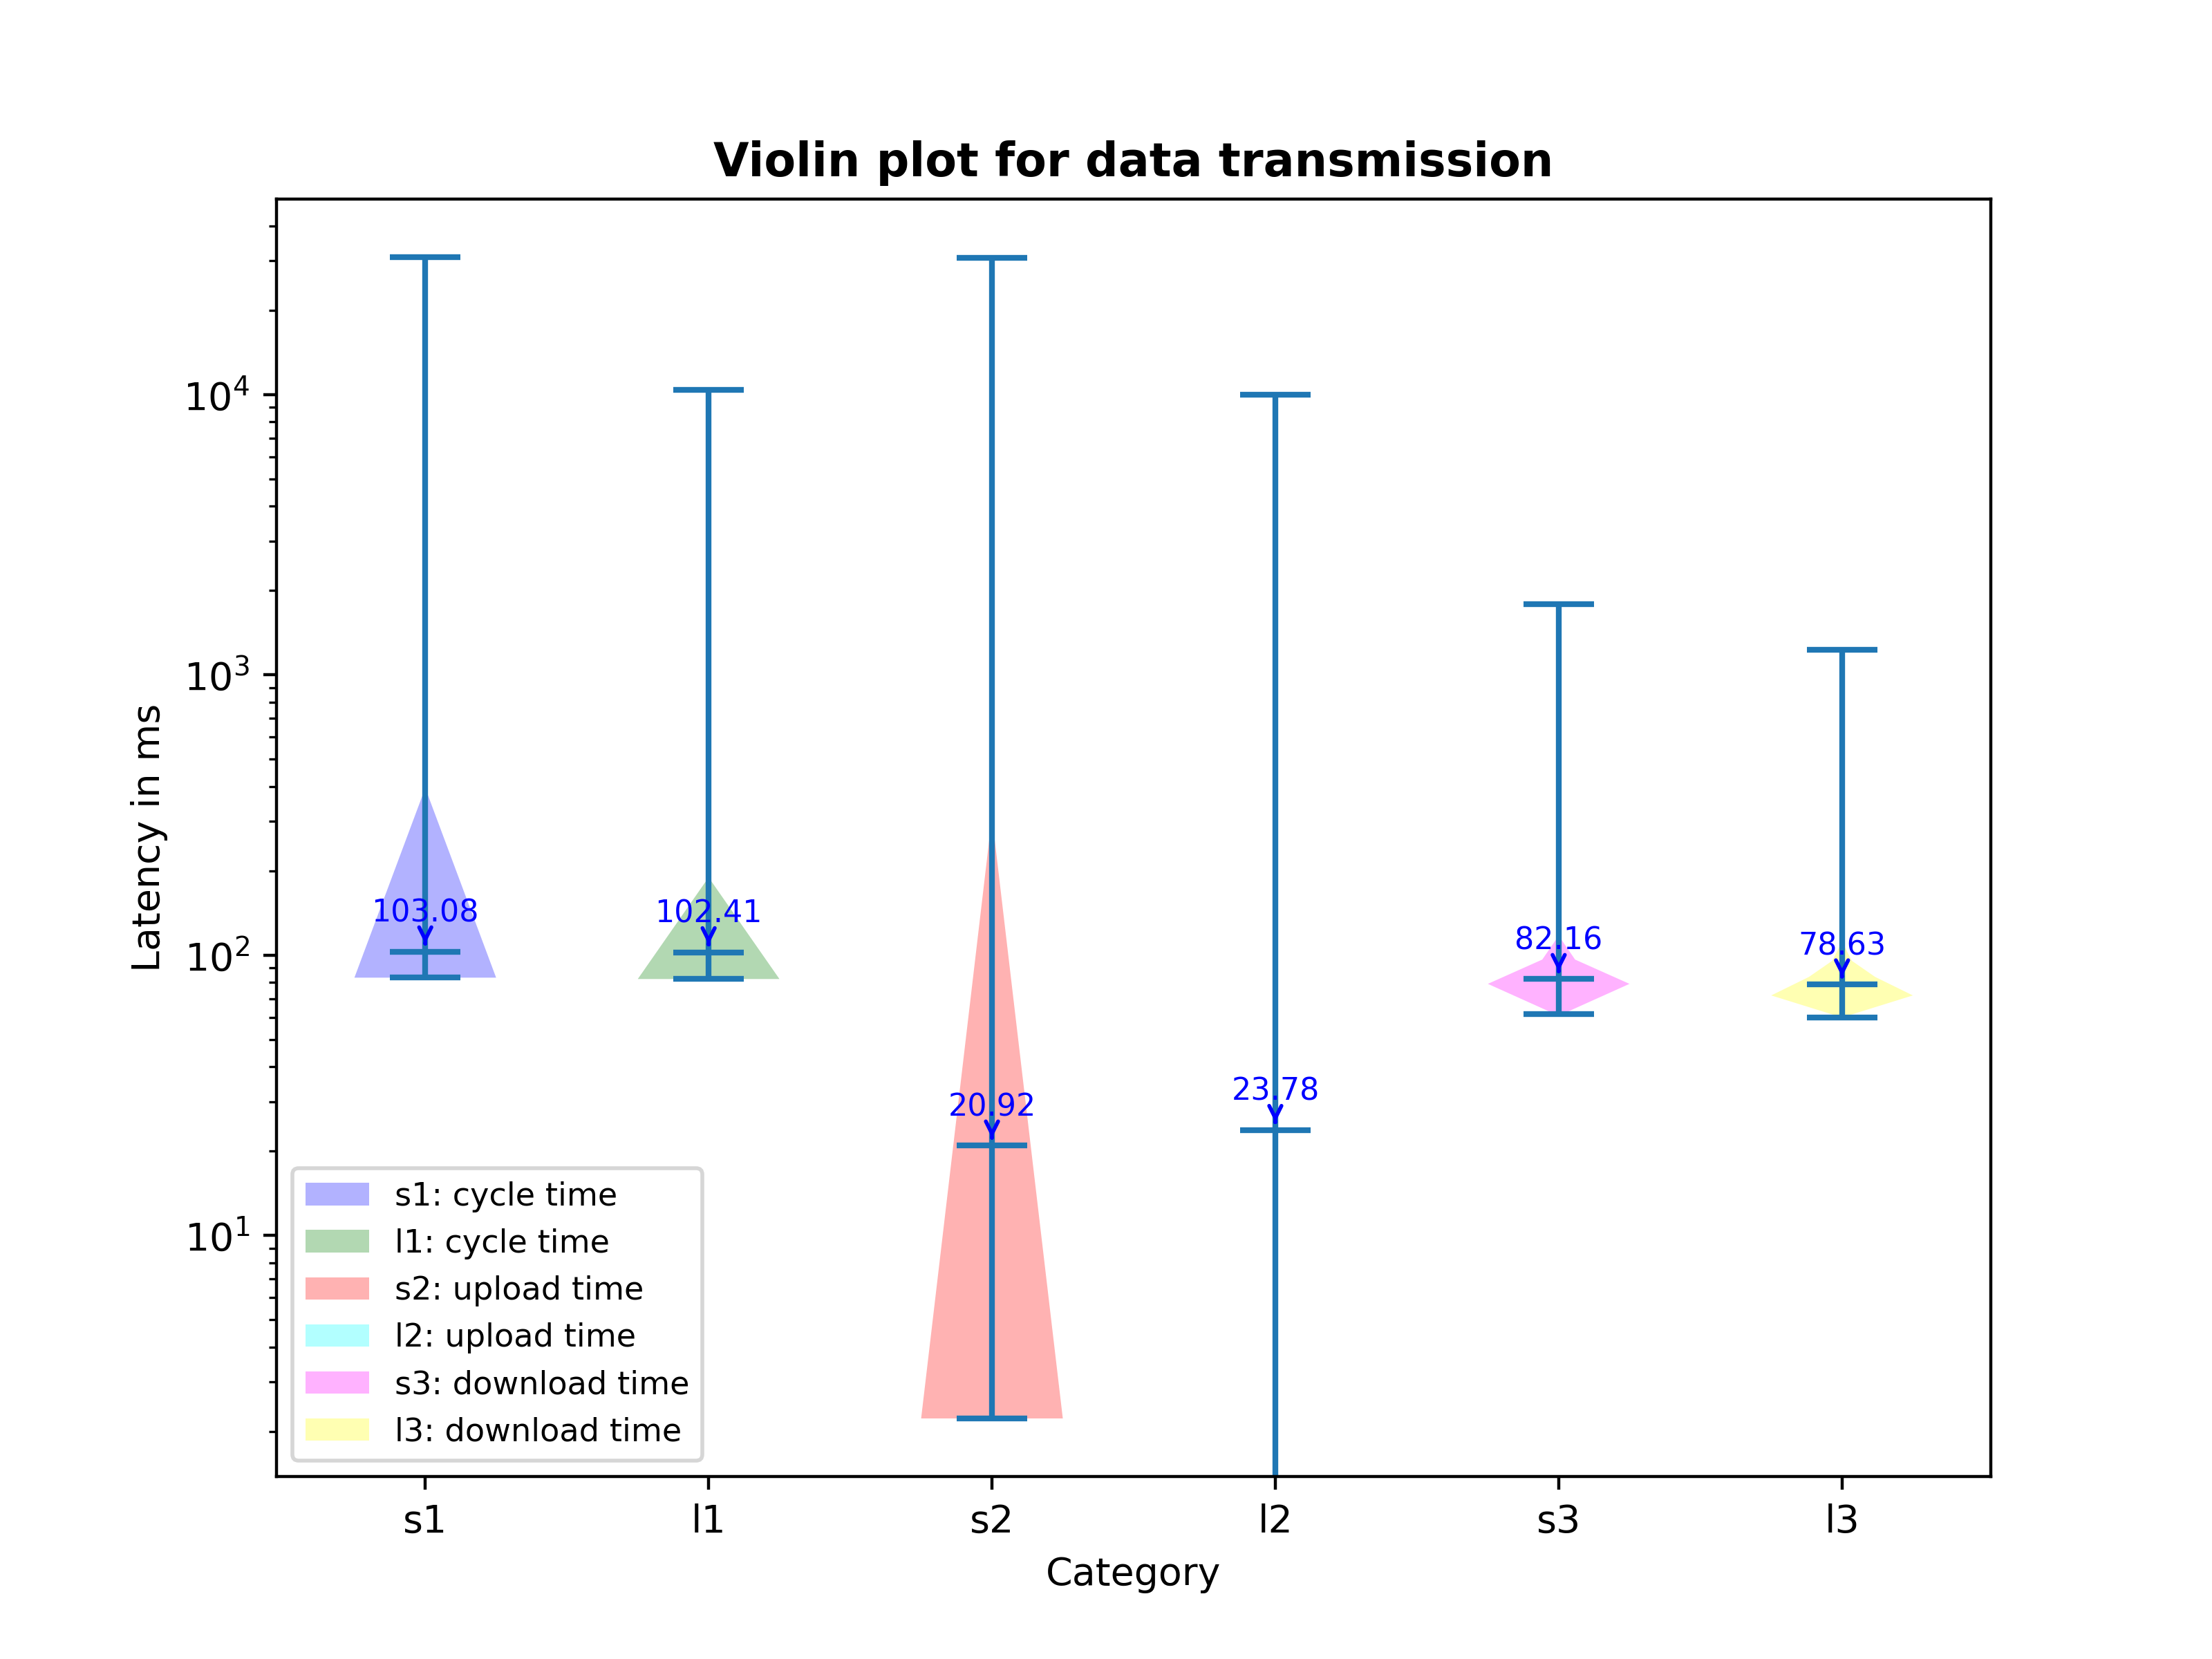
\includegraphics[width=\textwidth]{figures/tests/DT/violin_patch_size.png}
    \caption{Tests for \gls{rtt}, \gls{owd} from \gls{dta} to \gls{dt} 
    update of JointGripper, and \gls{owd} of twin value download for 
    two different patch sizes. In the graph, s represents small patches 
    and l for large patches.\label{fig: UD-violin-patchsize}}
\end{figure}

In general, the data upload and download time between \gls{dta} and the cloud is 
much higher than the field-level data transmission time under \gls{tcp} sockets. 
A fig.\ref{fig: SR-U-D-violin} shows the variance and mean of those in a violin plot 
for a more intuitive observation. 
Compared to the violin plot in fig.\ref{fig: UD-violin-patchsize}, the send and receive 
processes always show a symmetric triangular shape, suggesting a limited sample size. 
Considering the non-symmetric triangular shape of the uploading and downloading processes, 
it is likely to be attributed to the data points with a predominance at the lower extremum 
and the minimal presence at the upper extremum.
\begin{figure}[htb]
    \centering
    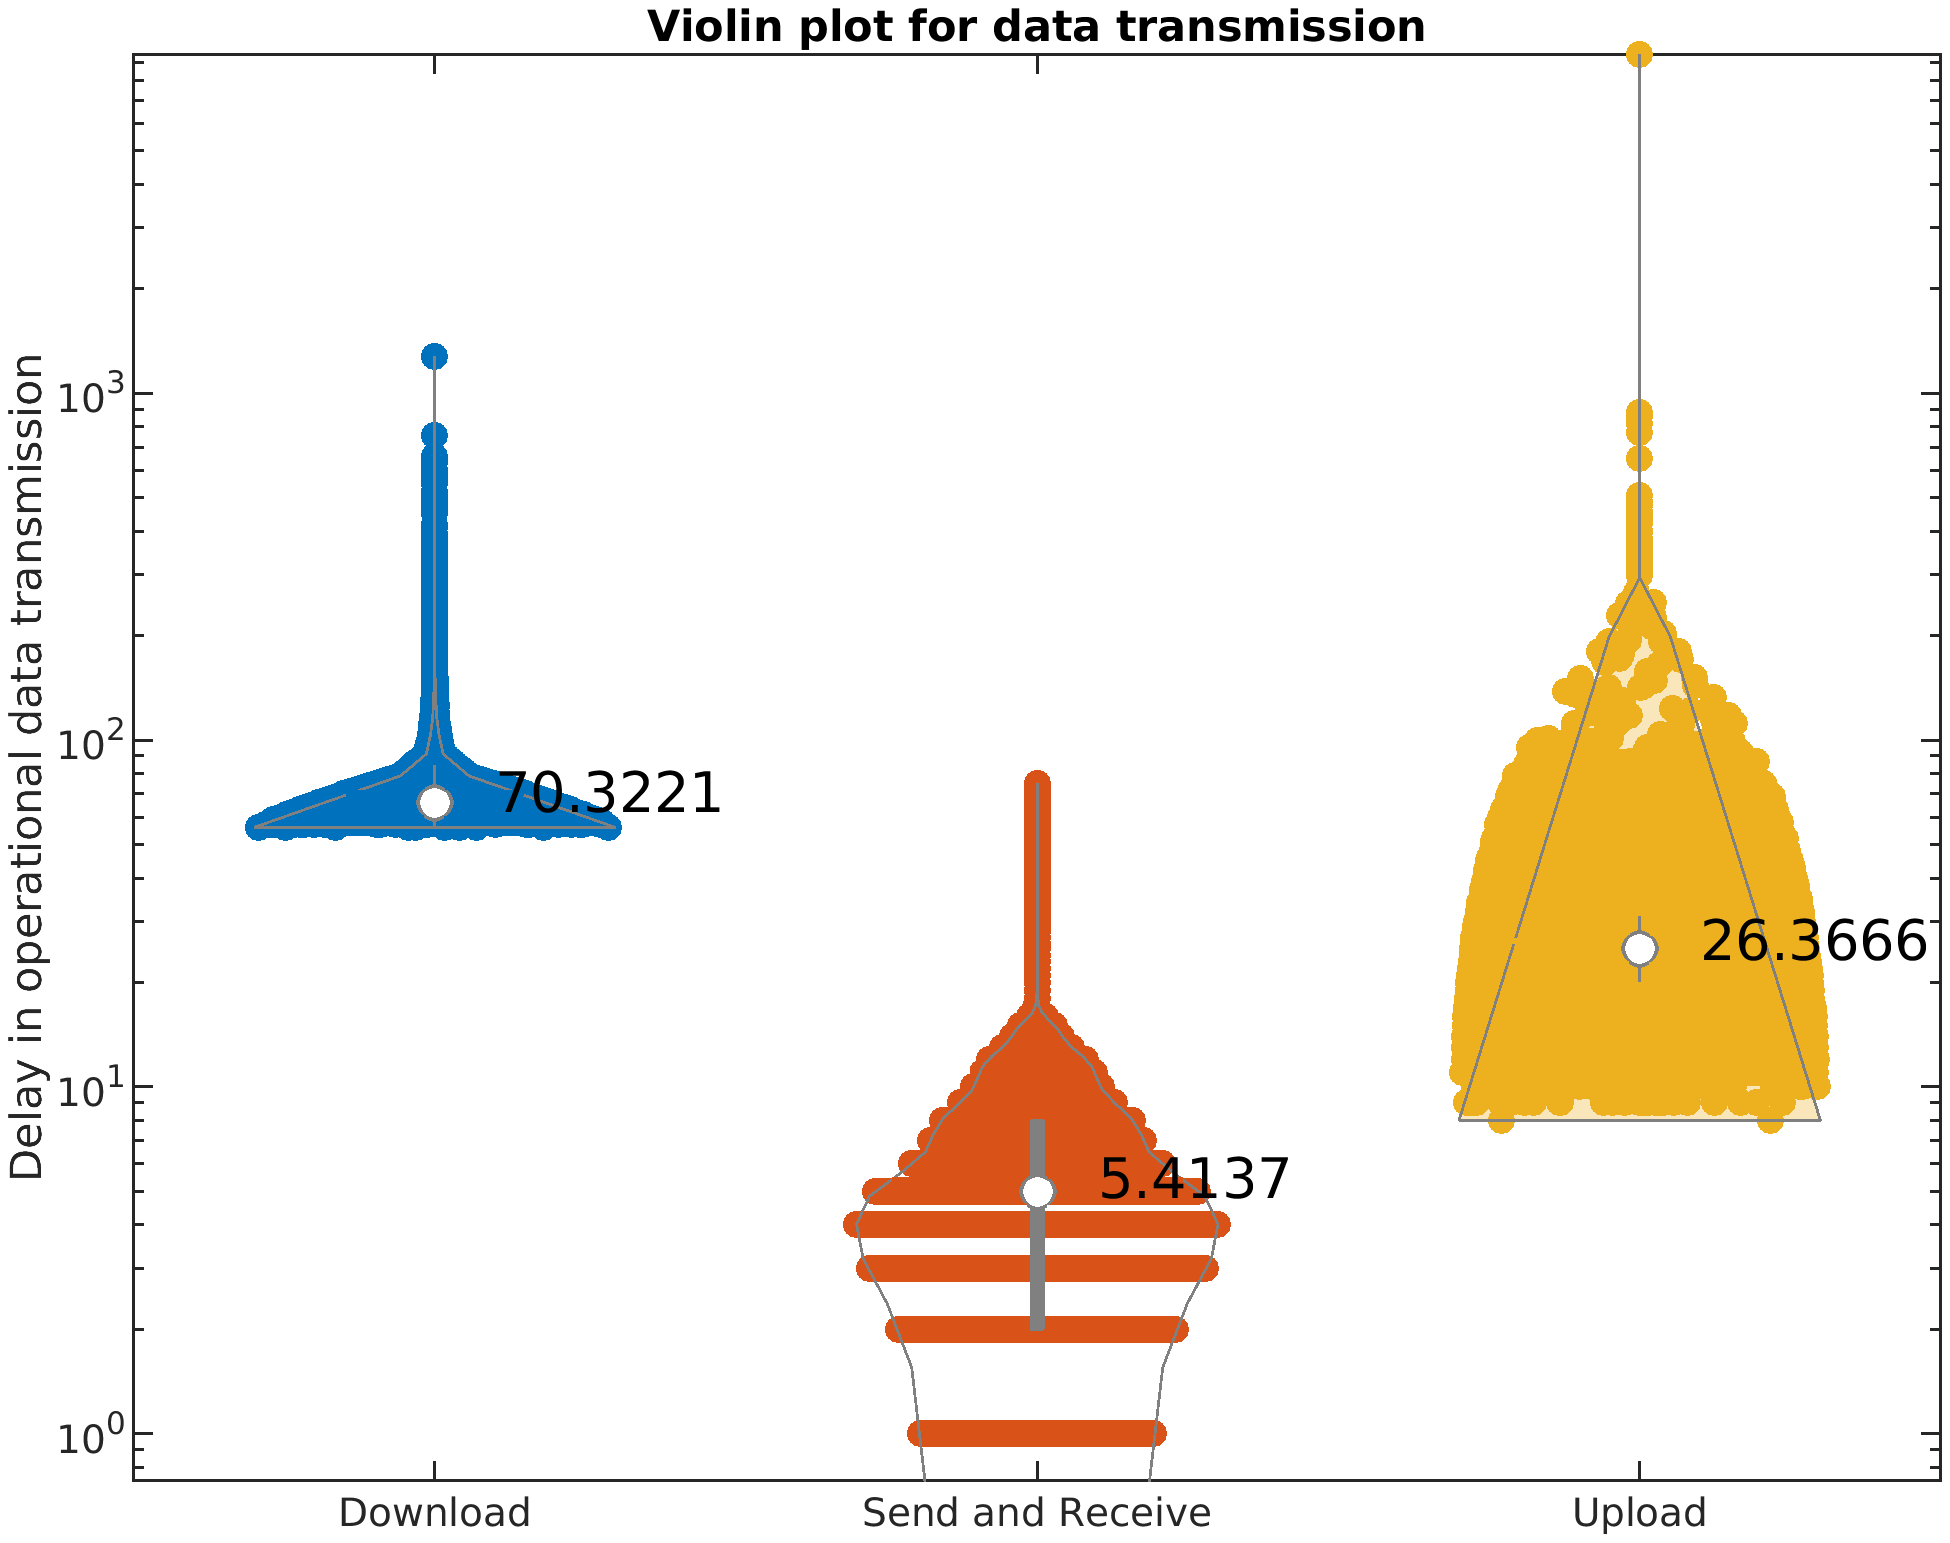
\includegraphics[width=\textwidth]{figures/tests/DT/log_violin_Plot_3cat.png}
    \caption{Tests for \gls{owd} from \gls{rcp} to \gls{dta}, 
    \gls{owd} from \gls{dta} to \gls{dt} 
    update of JointGripper, and \gls{owd} for twin value download.\label{fig: SR-U-D-violin}} 
\end{figure}


It is worth mentioning that, among all the tests for data update 
in the Azure \gls{dt} platform, there were several times that the 
twin instances experienced an incorrect update time. In these cases, 
the data update time is even earlier than the upload timestamp from the 
local device, which is theoretically impossible. The reason could be 
that the data update process in the cloud is operated internally but not necessarily in 
the same processing unit. The asynchronous processing in different counterparts 
can result in time synchronization issues. Also, the inaccuracy in the 
time synchronization across the devices and cloud servers may cause data 
inconsistency issues.



\section{Tests results overview}

For a more abstract overview, except for the use case-specific ones, all 
test results are listed in the following table \ref{tab: TestsProportional} to 
\ref{tab: TestsDT} for the horizontal and vertical comparison between 
one another. Table \ref{tab: TestsProportional} shows the tests results for 
WebSocket and \gls{http} by varying the conditions of the experiments 
while keeping the others unchanged. Similarly, tests conducted for message 
prioritization in the server are grouped in table \ref{tab: TestsPriority}, 
and the tests for global \gls{dt} are summarized in table \ref{tab: TestsDT}. 
The values in those tables are highly concentrated, with only the essential 
information included. A detailed view of all the experimental data refers to 
the repository. 
\footnote[3]{https://github.com/XuezhouHou/Websocket\_MAS/tree/master/Table\_with\_all\_values/Proportional\_test.xlsx}
\footnote[4]{https://github.com/XuezhouHou/Websocket\_MAS/tree/master/Table\_with\_all\_values/priority\_test.xlsx}
\footnote[5]{https://github.com/XuezhouHou/Websocket\_MAS/tree/master/Table\_with\_all\_values/DTA.xlsx}

% Please add the following required packages to your document preamble:
% \usepackage{graphicx}
% \usepackage[normalem]{ulem}
% \useunder{\uline}{\ul}{}
% \usepackage{lscape}

    \begin{table}[htbp]
    \footnotesize
    \centering
    \caption{An overview of tests for WebSocket and HTTP performance testing including worst case scenarios.}
    \label{tab: TestsProportional}
    \begin{tabular}{m{0.2\textwidth} m{0.08\textwidth} m{0.08\textwidth} m{0.08\textwidth} m{0.08\textwidth} m{0.08\textwidth} m{0.08\textwidth} m{0.08\textwidth}}
    \hline
    \textbf{Test case}                        & \textbf{var. value} & \textbf{Trans. Delay (ms)} & \textbf{OWD (ms)} & \textbf{Server Proc. Delay (ms)} & \textbf{Trans. Delay (ms)} & \textbf{OWD (ms)} & \textbf{Server Proc. Delay (ms)} \\ \hline
    1. Increase client\_Nr.          & 1          & 0.792             & 0.635    & 0.157                   & 0.782             & 0.629    & 0.153                   \\
    (server: 1,                      & 10         & 0.882             & 0.839    & 0.043                   & 0.548             & 0.515    & 0.034                   \\
    byte length: 40B,                & 100        & 4.610             & 4.548    & 0.062                   & 6.167             & 6.109    & 0.058                   \\
    protocol: WebSocket)             & 500        & 11.064            & 10.918   & 0.146                   & 21.681            & 21.540   & 0.141                   \\
                                     & 1000       & Timeout           & Timeout  & Timeout                 & Timeout           & Timeout  & Timeout                 \\
    & & & & & & &\\
    2. Increase server\_Nr.          & 2          & 1.538             & 1.394    & 0.144                   & 46.536            & 46.368   & 0.168                   \\
    (client: 1000, byte length: 40B, & 3          & 0.977             & 0.862    & 0.115                   & 55.024            & 54.918   & 0.106                   \\
    protocol: WS)                    &            &                   &          &                         &                   &          &                         \\
    & & & & & & &\\
    3. Increase string\_msg length   & 1KB        & 0.923             & 0.722    & 0.201                   & 0.936             & 0.737    & 0.199                   \\
    (client: 1,                      & 10KB       & 2.713             & 0.751    & 1.963                   & 3.128             & 0.946    & 2.182                   \\
    server: 1,                       & 100KB      & 19.848            & 0.769    & 19.079                  & 23.342            & 1.230    & 22.112                  \\
    protocol: WebSocket)             & 1MB        & 229.443           & 2.454    & 226.988                 & 253.098           & 4.122    & 248.976                 \\
                                     & 10MB       & 2789.003          & 28.481   & 2760.522                & 2834.665          & 31.330   & 2803.335                \\
                                     & 100MB      & Timeout           & Timeout  & Timeout                 & Timeout           & Timeout  & Timeout                 \\
    & & & & & & &\\
    4. Increase string\_msg length   &  1KB       & 2.294             & 1.525    & 0.768                   & 2.231             & 1.569    & 0.663                   \\
    (client: 1,                      &  10KB      & 7.331             & 5.380    & 1.951                   & 7.937             & 5.519    & 2.419                   \\
    server: 1,                       &  100KB     & 11.673            & 9.147    & 2.526                   & 12.528            & 9.652    & 2.876                   \\
    protocol: RESTful API)           &  1MB       & 51.967            & 49.963   & 2.003                   & 56.313            & 54.336   & 1.977                   \\
                                     &  10MB      & 362.932           & 359.836  & 3.096                   & 393.885           & 390.473  & 3.412                   \\
    & & & & & & &\\
    5. Increase JSON\_msg length     & 1KB        & 1.183             & 0.881    & 0.303                   & 1.226             & 0.881    & 0.346                   \\
    (client: 1,                      & 10KB       & 3.390             & 1.662    & 1.728                   & 3.488             & 1.662    & 1.826                   \\
    server: 1,                       & 100KB      & 11.848            & 5.306    & 6.542                   & 12.115            & 5.306    & 6.809                   \\
    protocol: WebSocket)             & 1MB        & 125.042           & 47.894   & 77.148                  & 117.523           & 47.894   & 69.629                  \\
                                     & 10MB       & 621.605           & 255.235  & 366.370                 & 654.673           & 255.235  & 399.438                 \\
                                     & 100MB      & 5810.514          & 1568.242 & 4242.272                & 5961.350          & 1568.242 & 4393.107                \\ \hline
    \end{tabular}%
    \end{table}



 % Please add the following required packages to your document preamble:
% \usepackage{graphicx}
% \usepackage{lscape}

    \begin{table}[htbp]
        \footnotesize
    \centering
    \caption{An overview of tests for message prioritization in WebSocket server with various performance testing.}
    \label{tab: TestsPriority}

    \begin{tabular}{m{0.2\textwidth} m{0.08\textwidth} m{0.08\textwidth} m{0.08\textwidth} m{0.08\textwidth} m{0.08\textwidth} m{0.08\textwidth} m{0.08\textwidth}}
        \hline
        \textbf{Test case}                     & \textbf{Client ID}  & \textbf{Trans. Delay (ms)} & \textbf{OWD (ms)}    & \textbf{Server Proc. Delay (ms)} & \textbf{Trans. Delay (ms)} & \textbf{OWD (ms)}    & \textbf{Server Proc. Delay (ms)} \\ \hline
        6. Non-priori. string\_msg    & 1-10       & 0.968   & 0.763  & 0.205   & 0.954   & 0.748  & 0.206   \\
        (client: 10,                  & (normal)   &         &        &         &         &        &         \\
        byte length: 40B,             &            &         &        &         &         &        &         \\
        Protocol: WebSocket)          &            &         &        &         &         &        &         \\
        & & & & & & &\\
        7. Non-priori. JSON\_msg      & 1-10       & 9.173   & 3.783  & 5.389   & 1.315   & 1.063  & 0.252   \\
        (byte length: 33.4KB,         & (normal)   &         &        &         &         &        &         \\
        Protocol: WebSocket)          &            &         &        &         &         &        &         \\
        & & & & & & &\\
        8. priori.string\_msg         & 1          & 31.391  & 1.140  & 30.251  & 973.309 & 1.193  & 972.116 \\
        (client: 2,                   & (normal)   &         &        &         &         &        &         \\
        byte length: 40B,             & 2          & 1.167   & 0.957  & 0.210   & 1.244   & 1.011  & 0.233   \\
        Protocol: WebSocket)          & (critical) &         &        &         &         &        &         \\
        & & & & & & &\\
        9. priori.string\_msg         & 1-9        & 115.323 & 2.789  & 112.534 & 69.841  & 1.789  & 68.052  \\
        (client: 10,                  & (normal)   &         &        &         &         &        &         \\
        byte length: 40B,             & 10         & 0.898   & 0.794  & 0.104   & 0.693   & 0.586  & 0.107   \\
        Protocol: WebSocket)          & (critical) &         &        &         &         &        &         \\
        & & & & & & &\\
        10. priori.string\_msg        & 1-49       & 28.700  & 3.090  & 25.610  & 12.079  & 3.435  & 8.644   \\
        (client: 50,                  & (normal)   &         &        &         &         &        &         \\
        byte length: 40B,             & 50         & 1.791   & 1.726  & 0.064   & 0.412   & 0.362  & 0.050   \\
        Protocol: WebSocket)          & (critical) &         &        &         &         &        &         \\
        & & & & & & &\\
        11. priori.JSON\_msg          & 1          & 393.123 & 4.344  & 388.779 & 243.836 & 3.113  & 240.723 \\
        (client: 2,                   & (normal)   &         &        &         &         &        &         \\
        (S/R byte length: 33.4KB/36B, & 2          & 12.781  & 4.293  & 8.488   & 2.635   & 2.331  & 0.305   \\
        Protocol: WebSocket)          & (critical) &         &        &         &         &        &         \\
        & & & & & & &\\
        12. priori.JSON\_msg          & 1-9        & 66.039  & 2.546  & 63.492  & 145.040 & 1.654  & 143.387 \\
        (client: 10,                  & (normal)   &         &        &         &         &        &         \\
        (S/R byte length: 33.4KB/36B, & 10         & 11.114  & 5.818  & 5.296   & 3.355   & 3.175  & 0.180   \\
        Protocol: WebSocket)          & (critical) &         &        &         &         &        &         \\
        & & & & & & &\\
        13. priori.JSON\_msg          & 1-49       & 84.425  & 10.530 & 73.895  & 31.434  & 23.069 & 8.365   \\
        (client: 50,                  & (normal)   &         &        &         &         &        &         \\
        (S/R byte length: 33.4KB/36B, & 50         & 27.577  & 22.481 & 5.097   & 4.277   & 4.094  & 0.183   \\
        Protocol: WebSocket)          & (critical) &         &        &         &         &        &         \\ \hline                   
    \end{tabular}%
    
    \end{table}



% Please add the following required packages to your document preamble:
% \usepackage{graphicx}
% \usepackage{lscape}

\begin{table}[htbp]
    \footnotesize
\centering
\caption{An overview of tests for data transport between \gls{rcp}, \gls{dta} and Azure \gls{dt}.}
\label{tab: TestsDT}

\begin{tabular}{m{0.36\textwidth} m{0.1\textwidth} m{0.1\textwidth} m{0.1\textwidth} m{0.1\textwidth}}
\hline
\textbf{Test case}                               & \textbf{var. value}   & \textbf{OWD forward (ms)} & \textbf{OWD return (ms)} & \textbf{RTT (ms)} \\ \hline
14. Var. string\_msg, RCP-DTA           & 151B         & 8.071  & None   & None    \\
(Protocol: TCP)                         & 80B          & 6.394  & None   & None    \\
                                        &              &        &        &         \\
15. Var. robot data, DTA-Azure DT       & JointGripper & 26.367 & 70.322 & 96.688  \\
(Protocol: HTTP/HTTPS,                  & Elbow        & 24.419 & 71.599 & 96.019  \\
msg type: JSON, byte length: 49B)       &              &        &        &         \\
                                        &              &        &        &         \\
16. Var. JSON\_msg, DTA-Azure DT        & 554B         & 20.920 & 82.160 & 103.080 \\
(Protocol: HTTP/HTTPS, data type: JSON) & 49B          & 23.780 & 78.630 & 102.410 \\
                                        &              &        &        &         \\
17. RCP-DTA-Azure DT                    & 151B         & 5.414  & None   & None    \\
(Protocols: TCP, HTTP/HTTPS;            & 49B          & 26.367 & 70.322 & 96.689  \\
msg type: string, JSON;                 &              &        &        &         \\
robot data: JointGripper)               &              &        &        &         \\ \hline
\end{tabular}%

\end{table}



